% This file makes a printable version of the blueprint
% It should include all the \usepackage needed for the pdf version.
% The template version assume you want to use a modern TeX compiler
% such as xeLaTeX or luaLaTeX including support for unicode
% and Latin Modern Math font with standard bugfixes applied.
% It also uses expl3 in order to support macros related to the dependency graph.
% It also includes standard AMS packages (and their improved version
% mathtools) as well as support for links with a sober decoration
% (no ugly rectangles around links).
% It is otherwise a very minimal preamble (you should probably at least
% add cleveref and tikz-cd).

\documentclass[a4paper]{article}

\usepackage{expl3}

\usepackage{amsmath, amssymb, amsthm, mathtools}
\usepackage[unicode,colorlinks=true,linkcolor=blue,urlcolor=magenta, citecolor=blue]{hyperref}

% \usepackage[warnings-off={mathtools-colon,mathtools-overbracket}]{unicode-math}
% \usepackage{fontspec}
% \setmathfont{latinmodern-math.otf}
% \setmathfont[range=\varnothing]{Asana-Math.otf}
% \setmathfont[range=\pitchfork]{Asana-Math.otf}
% \setmathfont[range=\intprod]{Asana-Math.otf}
% \setmathfont[range=\int]{latinmodern-math.otf}

\usepackage[capitalize,noabbrev]{cleveref}
\usepackage{autonum}

% \usepackage{tikz}
% \usepackage{tikz-cd}
\usepackage{graphicx} % Required for inserting images
% \usepackage{verbatim}

\usepackage{environ}

% Spacing and indentation

\usepackage{setspace}
\renewcommand{\baselinestretch}{1.5}

\usepackage[skip=12pt, indent=0pt]{parskip}
%\usepackage{indentfirst}

\allowdisplaybreaks  % Allows align environments to continue for several pages

% NOTE: PUT ALL MACROS IN macros/common.tex, macros/print.tex or macros/web.tex.

% In this file you should put all LaTeX macros to be used
% both by the pdf version and the web version.
% This should be most of your macros.

 % THEOREMS

\newtheorem{theorem}{Theorem}[section]
\newtheorem*{theorem*}{Theorem}
\newtheorem{corollary}[theorem]{Corollary}
\newtheorem{hypothesis}[theorem]{Hypothesis}
\newtheorem{proposition}[theorem]{Proposition}
\newtheorem{lemma}[theorem]{Lemma}
\newtheorem{definition}[theorem]{Definition}
\newtheorem{conjecture}[theorem]{Conjecture}
\newtheorem{example}[theorem]{Example}
\newtheorem{question}[theorem]{Question}
\newtheorem{remark}[theorem]{Remark}

% SET SYMBOLS

\newcommand{\R}{\mathbb{R}}
\newcommand{\Z}{\mathbb{Z}}
\newcommand{\C}{\mathbb{C}}
\newcommand{\N}{\mathbb{N}}
\newcommand{\h}{\mathfrak{H}}
\newcommand{\B}{\mathcal{B}}
\newcommand{\Pa}{\mathcal{P}}  % Sphere packing
\newcommand{\Vol}[1]{\operatorname{Vol}\!\left(#1\right)}

% DELIMITERS  % So we don't need to do \left, \right and possibly \middle when things are big (Sid)

\newcommand{\setof}[2]{\left\{ #1 \; \middle| \; #2 \right\}}

% \LEANtrue

\newcommand{\todo}[1]{{\color{red}{\textbf{#1}}}}

\newif\ifplastex

% This file makes a printable version of the blueprint
% It should include all the \usepackage needed for the pdf version.
% The template version assume you want to use a modern TeX compiler
% such as xeLaTeX or luaLaTeX including support for unicode
% and Latin Modern Math font with standard bugfixes applied.
% It also uses expl3 in order to support macros related to the dependency graph.
% It also includes standard AMS packages (and their improved version
% mathtools) as well as support for links with a sober decoration
% (no ugly rectangles around links).
% It is otherwise a very minimal preamble (you should probably at least
% add cleveref and tikz-cd).

\documentclass[a4paper]{article}

\usepackage{expl3}

\usepackage{amsmath, amssymb, amsthm, mathtools}
\usepackage[unicode,colorlinks=true,linkcolor=blue,urlcolor=magenta, citecolor=blue]{hyperref}

\usepackage[warnings-off={mathtools-colon,mathtools-overbracket}]{unicode-math}
\usepackage{fontspec}
\setmathfont{latinmodern-math.otf}
\setmathfont[range=\varnothing]{Asana-Math.otf}
\setmathfont[range=\pitchfork]{Asana-Math.otf}
\setmathfont[range=\intprod]{Asana-Math.otf}
\setmathfont[range=\int]{latinmodern-math.otf}

\usepackage[capitalize,noabbrev]{cleveref}
\usepackage{autonum}

% \usepackage{tikz}
% \usepackage{tikz-cd}
\usepackage{graphicx} % Required for inserting images

\usepackage{environ}

% NOTE: PUT ALL MACROS IN macros/common.tex, macros/print.tex or macros/web.tex.

% In this file you should put all LaTeX macros to be used
% both by the pdf version and the web version.
% This should be most of your macros.

 % THEOREMS

\newtheorem{theorem}{Theorem}[section]
\newtheorem*{theorem*}{Theorem}
\newtheorem{corollary}[theorem]{Corollary}
\newtheorem{hypothesis}[theorem]{Hypothesis}
\newtheorem{proposition}[theorem]{Proposition}
\newtheorem{lemma}[theorem]{Lemma}
\newtheorem{definition}[theorem]{Definition}
\newtheorem{conjecture}[theorem]{Conjecture}
\newtheorem{example}[theorem]{Example}
\newtheorem{question}[theorem]{Question}
\newtheorem{remark}[theorem]{Remark}

% SET SYMBOLS

\newcommand{\R}{\mathbb{R}}
\newcommand{\Z}{\mathbb{Z}}
\newcommand{\C}{\mathbb{C}}
\newcommand{\N}{\mathbb{N}}
\newcommand{\h}{\mathfrak{H}}
\newcommand{\B}{\mathcal{B}}
\newcommand{\Pa}{\mathcal{P}}  % Sphere packing
\newcommand{\Vol}[1]{\operatorname{Vol}\!\left(#1\right)}

% DELIMITERS  % So we don't need to do \left, \right and possibly \middle when things are big (Sid)

\newcommand{\setof}[2]{\left\{ #1 \; \middle| \; #2 \right\}}

% \LEANtrue

\newcommand{\todo}[1]{{\color{red}{\textbf{#1}}}}

\newif\ifplastex

% This file makes a printable version of the blueprint
% It should include all the \usepackage needed for the pdf version.
% The template version assume you want to use a modern TeX compiler
% such as xeLaTeX or luaLaTeX including support for unicode
% and Latin Modern Math font with standard bugfixes applied.
% It also uses expl3 in order to support macros related to the dependency graph.
% It also includes standard AMS packages (and their improved version
% mathtools) as well as support for links with a sober decoration
% (no ugly rectangles around links).
% It is otherwise a very minimal preamble (you should probably at least
% add cleveref and tikz-cd).

\documentclass[a4paper]{article}

\usepackage{expl3}

\usepackage{amsmath, amssymb, amsthm, mathtools}
\usepackage[unicode,colorlinks=true,linkcolor=blue,urlcolor=magenta, citecolor=blue]{hyperref}

\usepackage[warnings-off={mathtools-colon,mathtools-overbracket}]{unicode-math}
\usepackage{fontspec}
\setmathfont{latinmodern-math.otf}
\setmathfont[range=\varnothing]{Asana-Math.otf}
\setmathfont[range=\pitchfork]{Asana-Math.otf}
\setmathfont[range=\intprod]{Asana-Math.otf}
\setmathfont[range=\int]{latinmodern-math.otf}

\usepackage[capitalize,noabbrev]{cleveref}
\usepackage{autonum}

% \usepackage{tikz}
% \usepackage{tikz-cd}
\usepackage{graphicx} % Required for inserting images

\usepackage{environ}

% NOTE: PUT ALL MACROS IN macros/common.tex, macros/print.tex or macros/web.tex.

% In this file you should put all LaTeX macros to be used
% both by the pdf version and the web version.
% This should be most of your macros.

 % THEOREMS

\newtheorem{theorem}{Theorem}[section]
\newtheorem*{theorem*}{Theorem}
\newtheorem{corollary}[theorem]{Corollary}
\newtheorem{hypothesis}[theorem]{Hypothesis}
\newtheorem{proposition}[theorem]{Proposition}
\newtheorem{lemma}[theorem]{Lemma}
\newtheorem{definition}[theorem]{Definition}
\newtheorem{conjecture}[theorem]{Conjecture}
\newtheorem{example}[theorem]{Example}
\newtheorem{question}[theorem]{Question}
\newtheorem{remark}[theorem]{Remark}

% SET SYMBOLS

\newcommand{\R}{\mathbb{R}}
\newcommand{\Z}{\mathbb{Z}}
\newcommand{\C}{\mathbb{C}}
\newcommand{\N}{\mathbb{N}}
\newcommand{\h}{\mathfrak{H}}
\newcommand{\B}{\mathcal{B}}
\newcommand{\Pa}{\mathcal{P}}  % Sphere packing
\newcommand{\Vol}[1]{\operatorname{Vol}\!\left(#1\right)}

% DELIMITERS  % So we don't need to do \left, \right and possibly \middle when things are big (Sid)

\newcommand{\setof}[2]{\left\{ #1 \; \middle| \; #2 \right\}}

% \LEANtrue

\newcommand{\todo}[1]{{\color{red}{\textbf{#1}}}}

\newif\ifplastex

% This file makes a printable version of the blueprint
% It should include all the \usepackage needed for the pdf version.
% The template version assume you want to use a modern TeX compiler
% such as xeLaTeX or luaLaTeX including support for unicode
% and Latin Modern Math font with standard bugfixes applied.
% It also uses expl3 in order to support macros related to the dependency graph.
% It also includes standard AMS packages (and their improved version
% mathtools) as well as support for links with a sober decoration
% (no ugly rectangles around links).
% It is otherwise a very minimal preamble (you should probably at least
% add cleveref and tikz-cd).

\documentclass[a4paper]{article}

\usepackage{expl3}

\usepackage{amsmath, amssymb, amsthm, mathtools}
\usepackage[unicode,colorlinks=true,linkcolor=blue,urlcolor=magenta, citecolor=blue]{hyperref}

\usepackage[warnings-off={mathtools-colon,mathtools-overbracket}]{unicode-math}
\usepackage{fontspec}
\setmathfont{latinmodern-math.otf}
\setmathfont[range=\varnothing]{Asana-Math.otf}
\setmathfont[range=\pitchfork]{Asana-Math.otf}
\setmathfont[range=\intprod]{Asana-Math.otf}
\setmathfont[range=\int]{latinmodern-math.otf}

\usepackage[capitalize,noabbrev]{cleveref}
\usepackage{autonum}

% \usepackage{tikz}
% \usepackage{tikz-cd}
\usepackage{graphicx} % Required for inserting images

\usepackage{environ}

% NOTE: PUT ALL MACROS IN macros/common.tex, macros/print.tex or macros/web.tex.

\input{macros/common}
\input{macros/print}

\title{Sphere Packing in Lean}
\author{Maryna Viazovska}

\begin{document}
\maketitle
\input{content}
\end{document}


\title{Sphere Packing in Lean}
\author{Maryna Viazovska}

\begin{document}
\maketitle
% In this file you should put the actual content of the blueprint.
% It will be used both by the web and the print version.
% It should *not* include the \begin{document}
%
% If you want to split the blueprint content into several files then
% the current file can be a simple sequence of \input. Otherwise It
% can start with a \section or \chapter for instance.

\begin{abstract}
  In this paper we prove that no packing of unit balls in Euclidean space $\R^8$ has density greater than that of the $E_8$-lattice packing.
  \ifplastex
  % web
  The PDF version of this blueprint is available \href{https://thefundamentaltheor3m.github.io/Sphere-Packing-Lean/blueprint.pdf}{here}.
  \else
  % print
  The web version of this blueprint is available \href{https://thefundamentaltheor3m.github.io/Sphere-Packing-Lean/blueprint/index.html}{here}.
  \fi
  \end{abstract}


\section{Basic definitions for sphere packings}
\subsection{Sphere packings}
The sphere packing constant measures which portion of $d$-dimensional Euclidean
space can be covered by non-overlapping unit balls. More precisely, let $\R^d$ be the Euclidean vector space equipped with distance $\|\cdot\|$ and Lebesgue measure $\mathrm{Vol}(\cdot)$. For $x\in\R^d$ and $r\in\R_{>0}$ we denote by $B_d(x,r)$ the ball in $\R^d$ with center $x$ and radius $r$.

\begin{definition}\label{SpherePacking.isPacking}\lean{SpherePacking.isPacking}\leanok
  Let $X\subset \R^d$ be a discrete set of points such that $\|x-y\|\geq2$ for any distinct $x,y\in X$. Then the union
$$\mathcal{P}=\bigcup_{x\in X} B_d(x,1)$$ is a \emph{sphere packing}.
\end{definition}

\begin{definition}\label{SpherePacking.isLatticePacking}\uses{EuclideanLattice.is_lattice}\lean{SpherePacking.isLatticePacking}\leanok
  If $X$ is a lattice in $\R^d$ then we say that $\mathcal{P}$ is a \emph{lattice sphere packing}.
\end{definition}

\begin{definition}\label{SpherePacking.FiniteDensity}\lean{SpherePacking.FiniteDensity}\leanok
  The \emph{finite density} of a packing $\mathcal{P}$ is defined as
$$\Delta_{\mathcal{P}}(r):=\frac{\mathrm{Vol}(\mathcal{P}\cap B_d(0,r))}{\mathrm{Vol}(B_d(0,r))},\quad r>0.$$
\end{definition}

\begin{definition}\label{SpherePacking.Density}\uses{SpherePacking.FiniteDensity}\lean{SpherePacking.Density}\leanok
  We define the \emph{density} of a packing $\mathcal{P}$ as the limit superior
$$\Delta_{\mathcal{P}}:=\limsup\limits_{r\to\infty}\Delta_{\mathcal{P}}(r). $$
\end{definition}

\begin{definition}\label{SpherePacking.Constant}\uses{SpherePacking.isPacking, SpherePacking.Density}\lean{SpherePacking.Constant}\leanok
The number be want to know is the supremum over all possible packing densities
$$\Delta_d:=\sup\limits_{\substack{\mathcal{P}\subset\R^d\\ \scriptscriptstyle\mathrm{sphere}\;\mathrm{packing}}}\Delta_{\mathcal{P}} $$
called the \emph{sphere packing constant}.
\end{definition}

The main result of this paper is the proof that $$\Delta_8=\frac{\pi^4}{384}\approx 0.25367.$$
This is the density of the $E_8$-lattice sphere packing.

\begin{definition}\label{EuclideanLattice.E8}\lean{EuclideanLattice.E8}
  Recall that the $E_8$-lattice $\Lambda_8\subset\R^8$ is given by
$$\Lambda_8=\{(x_i)\in\Z^8\cup(\Z+\textstyle\frac12\displaystyle )^8|\;\sum_{i=1}^8x_i\equiv 0\;(\mathrm{mod\;2})\}.$$
\end{definition}
\begin{lemma}\label{lemma: Characterisation of E8 lattice}
  $\Lambda_8$ is a positive-definite, even, unimodular lattice of rank 8. The minimal distance between two points in $\Lambda_8$ is $\sqrt{2}$.
\end{lemma}
\begin{definition}\label{SpherePacking.E8}\uses{EuclideanLattice.E8}\lean{SpherePacking.E8}\leanok
The $E_8$-lattice sphere packing is the packing of unit balls with centers at $\frac{1}{\sqrt{2}}\Lambda_8$.
\end{definition}
Our main result is
\begin{theorem}\label{SpherePacking.Main}\lean{SpherePacking.Main}
No packing of unit balls
in Euclidean space $\R^8$ has density greater than that of the $E_8$-lattice packing.
\end{theorem}

\subsection{Lattices and Periodic packings}
\begin{definition}\label{def: Periodicity}
  Let $S$ be a discrete subgroup of $\R^d$. A set $X\subset\R^d$ is said to $S$-periodic if for each $s\in S$ and $x\in X$ the vector $x+s$ belongs to $X$.
\end{definition}

\begin{definition}\label{EuclideanLattice.is_lattice}\lean{EuclideanLattice.is_lattice}\leanok
  % A lattice in the Euclidean space $\R^d$ is a discrete, co-compact, abelian subgroup.
  A subset of the Euclidean space $\R^d$ is called a lattice if it is the $\Z$-span of a basis of $\R^d$.
\end{definition}

\begin{lemma}\label{SpherePacking.Density of periodic packing} \notready
  Density of a periodic packing ...
\end{lemma}
\subsection{Facts from Fourier analysis}
hello
In this subsection we recall a few definitions from Fourier analysis.
\begin{definition}\label{def: Fourier Transform definition} % \lean{def: Fourier Transform definition}
The Fourier transform of an $L^1$-function $f:\R^d\to\C$ is defined as
$$\mathcal{F}(f)(y)=\widehat{f}(y):=\int\limits_{\R^d} f(x)\,e^{-2\pi i x\cdot y}\,dx,\quad y\in\R^d $$
where $x\cdot y=\frac12\|x\|^2+\frac12\|y\|^2-\frac12\|x-y\|^2$ is the standard scalar product in $\R^d$.
\end{definition}
\begin{definition}
A $C^\infty$~function $f:\R^d\to\C$ is called a \emph{Schwartz function} if it goes to zero as $\|x\|\to\infty$ faster then any inverse power of $\|x\|$, and the same holds for all partial derivatives of $f$. The set of all Schwartz functions is called a \emph{Schwartz space}.
\end{definition}
\begin{lemma}\label{lemma: Fourier transform is automorphism}
  The Fourier transform is an automorphism of the space of Schwartz functions.
\end{lemma}
\begin{lemma}\label{lemma: Gaussian Fourier}\uses{def: Fourier Transform definition}
\begin{equation}\mathcal{F}(e^{\pi i  \|x\|^2 z})(y)=z^{-4}\,e^{\pi i \|y\|^2 \,(\frac{-1}{z}) }.\end{equation}
\end{lemma}
\begin{theorem}\label{thm: Poisson summation formula}\uses{def: Fourier Transform definition}
  (Poisson summation formula)$$\sum_{\ell\in\Lambda}f(\ell)=\frac{1}{\mathrm{vol}(\R^d/\Lambda)}\sum_{m\in\Lambda^*}\widehat{f}(m).$$
\end{theorem}

\section{Cohn-Elkies linear programming bounds}

In 2003 Cohn and Elkies \cite{ElkiesCohn}  developed  linear programming bounds that apply directly to sphere packings. The goal of this section is to formalize the Cohn--Elkies linear programming bound.

The following theorem is the key result of \cite{ElkiesCohn}. (The original theorem is stated for a   class of functions more general then Schwartz functions)
\begin{theorem}\label{thm: Cohn-Elkies}\uses{def: Fourier Transform definition}\uses{thm: Poisson summation formula}
(Cohn, Elkies \cite{ElkiesCohn}) Suppose that  $f:\R^d\to\R$ is a Schwartz function, is not identically zero, and satisfies:
\begin{equation}\label{eqn: Cohn-Elkies condition 1}f(x)\leq 0\mbox{ for } \|x\|\geq 1\end{equation} and
\begin{equation}\label{eqn: Cohn-Elkies condition 2}\widehat{f}(x)\geq0\mbox{ for all } x\in\R^d.\end{equation}
  Then the  density of  $d$-dimensional
  sphere packings is bounded above by $$\frac{f(0)}{\widehat{f}(0)}\cdot \frac{\pi^{\frac{d}{2}}}{2^d\,\Gamma(\textstyle \frac{d}{2}+1)}.$$
\end{theorem}
\begin{proof}
To be included.
\end{proof}


  The main step in our proof of Theorem \ref{SpherePacking.Main} is the explicit  construction of an optimal function. It will be convenient for us to scale this function by $\sqrt{2}$.
\begin{theorem}\label{thm: g}
There exists a radial Schwartz function $g:\R^8\to\R$ which satisfies:
\begin{align}
g(x)&\leq 0\mbox{ for } \|x\|\geq \sqrt{2} \label{eqn: g1}\\
\widehat{g}(x)&\geq0\mbox{ for all } x\in\R^8\label{eqn: g2}\\
g(0)&=\widehat{g}(0)=1.\label{eqn: g3}
\end{align}
\end{theorem}
Theorem \ref{thm: Cohn-Elkies} applied to the optimal function $f(x)=g(x/\sqrt{2})$ immediately implies Theorem \ref{SpherePacking.Main}.


\section{Modular forms}
Let $\h$ be the upper half-plane $\{z\in\C\mid\Im(z)>0\}$. The modular group $\Gamma_1:=\mathrm{PSL}_2(\Z)$ acts on $\h$ by linear fractional transformations
$$\left(\begin{smallmatrix}a&b\\c&d\end{smallmatrix}\right)z:=\frac{az+b}{cz+d}.$$

Let $N$ be a positive integer. The \emph{level $N$ principal congruence subgroup} of $\Gamma_1$ is
$$\Gamma(N):=\left\{\left.\left(\begin{smallmatrix}a&b\\c&d\end{smallmatrix}\right)\in\Gamma_1\right|\left(\begin{smallmatrix}a&b\\c&d\end{smallmatrix}\right)\equiv\left(\begin{smallmatrix}1&0\\0&1\end{smallmatrix}\right)\;\mathrm{mod}\;N\right\}.$$
A subgroup $\Gamma\subset\Gamma_1$ is called a \emph{congruence subgroup} if $\Gamma(N)\subset\Gamma$ for some $N\in\N$. An important example of a congruence subgroup is
$$\Gamma_0(N):=\left\{\left.\left(\begin{smallmatrix}a&b\\c&d\end{smallmatrix}\right)\in\Gamma_1\right|\;c\equiv0\;\mathrm{mod}\;N\right\}.$$

Let $z\in\h$, $k\in\Z$, and $\left(\begin{smallmatrix}a&b\\c&d\end{smallmatrix}\right)\in\mathrm{SL}_2(\Z)$. The \emph{automorphy factor} of weight $k$ is defined as
$$j_k(z,\left(\begin{smallmatrix}a&b\\c&d\end{smallmatrix}\right)):=(cz+d)^{-k}.$$
The automorphy factor satisfies the \emph{chain rule}
$$j_k(z,\gamma_1\gamma_2)=j_k(z,\gamma_1)\,j_k(\gamma_2z,\gamma_1). $$
Let $F$ be a  function on $\h$ and $\gamma\in\mathrm{PSL}_2(\Z)$. Then the \emph{slash operator} acts on $F$ by
$$(F|_k\gamma)(z):=j_k(z,\gamma)\,F(\gamma z). $$
The chain rule implies
$$F|_k\gamma_1\gamma_2=(F|_k\gamma_1)|_k\gamma_2.$$

\begin{definition}\label{def: holomorphic modular form}% \lean{def: holomorphic modular form}
A \emph{(holomorphic) modular form} of integer weight $k$ and congruence subgroup $\Gamma$ is a holomorphic function $f:\h\to\C$ such that:
\begin{enumerate}
  \item $f|_k\gamma=f$ for all $\gamma\in\Gamma$
  \item for each $\alpha\in\Gamma_1\;f|_k\alpha$ has the Fourier expansion $f|_k\alpha (z)=\sum_{n=0}^\infty c_f(\alpha,\frac{n}{n_\alpha})\,e^{2\pi i \frac{n}{n_\alpha}z}$ for some $n_\alpha\in\N$ and Fourier coefficients $c_f(\alpha,m)\in\C$.
\end{enumerate}
\end{definition}

Let $M_k(\Gamma)$ be the space of modular forms of weight $k$ and congruence subgroup $\Gamma$. A key fact in the theory of modular forms is that the spaces $M_k(\Gamma)$ are finite dimensional.

Let us consider several examples of modular forms.
\begin{definition}\label{def: Ek definition}% \lean{def: Ek definition}
For an even integer $k\geq 4$ we define the \emph{weight $k$ Eisenstein series} as
\begin{equation}\label{eqn: Ek definition}E_k(z):=\frac{1}{2\zeta(k)}\sum_{(c,d)\in\Z^2\backslash(0,0)}(c\tau+d)^{-k}.\end{equation}
\end{definition}
Since the sum converges absolutely, it is easy to see that $E_k\in M_k(\Gamma_1)$.
\begin{lemma}\label{lemma: Ek Fourier}
% \lean{lemma: Ek Fourier}\uses{def: Ek definition}
The Eisenstein series possesses the Fourier expansion
\begin{equation}\label{eqn: Ek Fourier}E_k(z)=1+\frac{2}{\zeta(1-k)}\sum_{n=1}^\infty \sigma_{k-1}(n)\,e^{2\pi i z}, \end{equation}
where $\sigma_{k-1}(n)\,=\,\sum_{d|n} d^{k-1}$. In particular, we have
\begin{align}
  E_4(z)\,=\,& 1+240\sum_{n=1}^\infty \sigma_3(n)\,e^{2\pi i n z} \notag \\
  E_6(z)\,=\,& 1-504\sum_{n=1}^\infty \sigma_5(n)\,e^{2\pi i n z}. \notag
\end{align}
\end{lemma}
The infinite sum \eqref{eqn: Ek definition} does not converge absolutely for $k=2$. On the other hand, the expression \eqref{eqn: Ek Fourier} converges to a holomorphic function on the upper half-plane and therefore
\begin{definition} \label{def: E2 def} % \lean{def: E2 def}
We set
\begin{equation}E_2(z):= 1-24\sum_{n=1}^\infty \sigma_1(n)\,e^{2\pi i n z}.\notag\end{equation}
\end{definition}
\begin{lemma}
\label{lemma: E2 transform}

% \lean{lemma: Ek Fourier}

This function is not modular, however it satisfies
\begin{equation}\label{eqn: E2 transform}z^{-2}\,E_2\Big(\frac{-1}{z}\Big)=E_2(z) -\frac{6i}{\pi}\, \frac{1}{z}.\end{equation}
\end{lemma}
The proof of this identity can be found in \cite[Section~2.3]{1-2-3}.
The weight two Eisenstein series $E_2$ is an example of a \emph{quasimodular form} \cite[Section~5.1]{1-2-3}.

Another example of modular forms we would like to consider are \emph{theta functions} \cite[Section~3.1]{1-2-3}.
We define three different theta functions (so called ``Thetanullwerte'') as
\begin{align}
  \theta_{00}(z)\,=\, & \sum_{n\in\Z}e^{\pi i n^2 z} \notag \\
  \theta_{01}(z)\,=\, & \sum_{n\in\Z}(-1)^n\,e^{\pi i n^2 z} \notag \\
  \theta_{10}(z)\,=\, & \sum_{n\in\Z}e^{\pi i (n+\frac12)^2 z}. \notag
\end{align}
The group $\Gamma_1$ is generated by the elements $T=\left(\begin{smallmatrix}1&1\\0&1\end{smallmatrix}\right)$ and $S=\left(\begin{smallmatrix}0&1\\-1&0\end{smallmatrix}\right)$.
\begin{lemma}\label{lemma: theta transform S T}
% \lean{lemma: theta transform S T}

These elements  act on the theta functions in the following way
\begin{align}
z^{-2}\,\theta^4_{00}\Big(\frac{-1}{z}\Big)\,=\,&-\theta_{00}^4(z) \label{eqn: theta transform S}\\
z^{-2}\,\theta^4_{01}\Big(\frac{-1}{z}\Big)\,=\,&-\theta_{10}^4(z)\\
z^{-2}\,\theta^4_{10}\Big(\frac{-1}{z}\Big)\,=\,&-\theta_{01}^4(z)
\end{align}
and
\begin{align}
\theta^4_{00}(z+1)\,=\,&\theta_{01}^4(z)\\
\theta^4_{01}(z+1)\,=\,&\theta_{00}^4(z)\\
\theta^4_{10}(z+1)\,=\,&-\theta_{10}^4(z). \label{eqn: theta transform T}
\end{align}
\end{lemma}
Moreover, these three theta functions satisfy the \emph{Jacobi identity}
\begin{equation}
\theta_{01}^4+\theta_{10}^4=\theta_{00}^4.
\end{equation}
The theta functions $\theta^4_{00},\theta^4_{01}$, and $\theta^4_{10}$ belong to $M_2(\Gamma(2))$.


\begin{definition}\label{def: weakly-holomorphic modular form}
A \emph{weakly-holomorphic modular form} of integer weight $k$ and congruence subgroup $\Gamma$ is a holomorphic function $f:\h\to\C$ such that:
\begin{enumerate}
  \item $f|_k\gamma=f$ for all $\gamma\in\Gamma$
  \item for each $\alpha\in\Gamma_1\;f|_k\alpha$ has the Fourier expansion $f|_k\alpha (z)=\sum_{n=n_0}^\infty c_f(\alpha,\frac{n}{n_\alpha})\,e^{2\pi i \frac{n}{n_\alpha}z}$ for some $n_0\in\Z$ and $n_\alpha\in\N$.
\end{enumerate}
\end{definition}
For an $m$-periodic holomorphic function $f$ and $n\in\frac 1m \Z$ we will denote the $n$-th Fourier coefficient of $f$ by $c_f(n)$ so that
$$f(z)=\sum_{n\in\frac 1m \Z} c_f(n)\,e^{2\pi i n z}.$$
We denote the space of weakly-holomorphic modular forms of weight $k$ and group $\Gamma$ by $M_k^!(\Gamma)$. The spaces $M_k^!(\Gamma)$ are infinite dimensional.
Probably the most famous weakly-holomorphic modular form is the \emph{elliptic j-invariant}
$$j\,:=\,\frac{1728\, E_4^3}{E_4^3-E_6^2}. $$
This function belongs to $M_0^!(\Gamma_1)$ and has the Fourier expansion
$$j(z)\,=\,q^{-1} + 744 + 196884\, q + 21493760\, q^2 + 864299970\, q^3 +
  20245856256\, q^4 + O(q^5) $$
  where $q=e^{2\pi i z}$. Using a simple computer algebra system such as PARI GP or Mathematica one can compute first hundred terms of this Fourier expansion within few seconds. An important question is to find an  asymptotic formula for $c_j(n)$, the $n$-th Fourier coefficient  of $j$. Using the Hardy-Ramanujan circle method \cite{Rademacher38} or the non-holomorphic Poincare series \cite{Petersson32} one can show that
  \begin{lemma}\label{lemma: j Fourier asymptotic}
  % \lean{lemma: j Fourier asymptotic}
  \begin{equation}\label{eqn: j Fourier asymptotic}
  c_j(n)=\frac{2\pi}{n}\sum_{k=1}^\infty \frac{A_k(n)}{k}\,I_1\left(\frac{4\pi \sqrt{n}}{k}\right)\qquad n\in\Z_{>0}\end{equation}
  where
  $$A_k(n)= \sum_{\substack{h\;\mathrm{mod}\;k\\(h,k)=1}} e^{\frac{-2\pi i}{k}(nh+h')},\quad hh'\equiv -1(\mbox{mod}\;k),$$
  and $I_\alpha(x)$ denotes the modified Bessel function of the first kind defined as in \cite[Section~9.6]{Abramowitz}.
  \end{lemma}
  A similar convergent asymptotic expansion holds for the Fourier coefficients of any weakly holomorphic modular form \cite{Hejhal}, \cite[Propositions~1.10 and~1.12]{Bruinier}. Such a convergent expansion implies effective estimates for the Fourier coefficients.




\section{Fourier eigenfunctions with double zeroes at lattice points}\label{sec: fourier double zeroes}
In this section we construct two radial Schwartz functions $a,b:\R^8\to i\R$ such that
\begin{align}\mathcal{F}(a)&=a\label{eqn: a fourier}\\
  \mathcal{F}(b)&=-b\label{eqn: b fourier}
\end{align}
which double zeroes at all $\Lambda_8$-vectors of length greater than $\sqrt{2}$. Recall that each vector of $\Lambda_8$ has length $\sqrt{2n}$ for some $n\in\N_{\geq 0}$. We define $a$ and $b$ so that their values are purely imaginary because this simplifies some of our computations. We will show in Section \ref{sec: g} that an appropriate linear combination of functions $a$ and $b$ satisfies conditions \eqref{eqn: g1}--\eqref{eqn: g3}.

First, we will define function $a$. To this end we consider the following functions:
\begin{definition}\label{def: phi4 phi2 phi0}
\uses{def: Ek definition}
\begin{align}
  \phi_{-4}\,:= \,& -Dj\,E_6^{-1}\label{eqn: def phi4}\\
  \phi_{-2}\,:= \,&\phi_{-4}\,E_2+Dj\,E_4^{-1}\label{eqn: def phi2}\\
  \phi_{0}\,:= \,&\phi_{-4}\,E_2^2+2Dj\,E_4^{-1}\,E_2+j-1728.\label{eqn: def phi0}
\end{align}
\end{definition}
Here $Dj(z)=\frac{1}{2\pi i} \frac{d}{dz} j(z)$.
\begin{lemma}\label{lemma: phi fourier4 phi fourier2 phi fourier0}
  These functions have the Fourier expansions
\begin{align}
  \phi_{-4}(z)\,=\,&q^{-1} + 504 + 73764\, q + 2695040\, q^2 + 54755730\, q^3 + O(q^4)\label{eqn: phi fourier4}\\
  \phi_{-2}(z)\,=\,&720 + 203040\, q + 9417600\, q^2 + 223473600\, q^3 + 3566782080\, q^4+O(q^5)\label{eqn: phi fourier2}\\
  \phi_{0}(z)\,=\,&518400\, q + 31104000\, q^2 + 870912000\, q^3 + 15697152000\, q^4+O(q^5)\label{eqn: phi fourier0}
\end{align}
where $q=e^{2\pi i z}$.
\end{lemma}
The function $\phi_0(z)$ is not modular; however,
\begin{lemma}\label{lemma: phi0 transform}
  The identity \ref{lemma: E2 transform} implies the following transformation rule:
\begin{equation}\label{eqn: phi0 transform}
\phi_0\Big(\frac{-1}{z}\Big)=\phi_0(z)-\frac{12i}{\pi}\,\frac{1}{z}\,\phi_{-2}(z)-\frac{36}{\pi^2}\,\frac{1}{z^2}\,\phi_{-4}(z).
\end{equation}
\end{lemma}
\begin{definition}\label{def: a(r) definition}
For $x\in\R^8$ we define
\begin{align}\label{eqn: a(r) definition}
  a(x):=&\int\limits_{-1}^i\phi_0\Big(\frac{-1}{z+1}\Big)\,(z+1)^2\,e^{\pi i \|x\|^2 z}\,dz
  +\int\limits_{1}^i\phi_0\Big(\frac{-1}{z-1}\Big)\,(z-1)^2\,e^{\pi i \|x\|^2 z}\,dz\\
  -&2\int\limits_{0}^i\phi_0\Big(\frac{-1}{z}\Big)\,z^2\,e^{\pi i \|x\|^2 z}\,dz
  +2\int\limits_{i}^{i\infty}\phi_0(z)\,e^{\pi i \|x\|^2 z}\,dz.\nonumber
\end{align}
\end{definition}
We observe that the contour integrals in \eqref{eqn: a(r) definition} converge absolutely and uniformly for  $x\in\R^8$. Indeed,
$\phi_0(z)=O(e^{-2\pi i z})$ as $\Im(z)\to \infty$. Therefore, $a(x)$ is well defined. Now we prove that $a$ satisfies condition \eqref{eqn: a fourier}.
\begin{proposition}\label{prop: a(r) Fourier}\uses{lemma: Ek Fourier}\uses{def: E2 def}\uses{lemma: j Fourier asymptotic}\uses{def: a(r) definition}\uses{lemma: Gaussian Fourier}

The function $a$ defined by \eqref{eqn: a(r) definition} belongs to the Schwartz space and satisfies $$\widehat{a}(x)=a(x). $$
\end{proposition}
\begin{proof}
First, we prove that $a$ is a Schwartz function. From Lemma \ref{lemma: Ek Fourier}, Definition \ref{def: E2 def}, and \ref{lemma: j Fourier asymptotic} we deduce that the Fourier coefficients of $\phi_0$ satisfy
$$|c_{\phi_0}(n)|\leq2\,e^{4\pi\sqrt{n}}\quad n\in\Z_{>0}.$$ Thus, there exists a positive constant $C$ such that
$$|\phi_0(z)|\leq C\,e^{-2\pi \Im{z}}\qquad \mbox{for } \; \Im{z}>\frac 12.$$
We estimate the first summand in the right-hand side of \eqref{eqn: a(r) definition}.  For $r\in\R_{\geq 0}$ we have
\begin{align}&\Bigg|\int\limits_{-1}^{i}\phi_0\Big(\frac{-1}{z+1}\Big)\,(z+1)^2\,e^{\pi i r^2 z}\,dz\Bigg|=\Bigg|\int\limits_{i\infty}^{-1/(i+1)}\phi_0(z)\,z^{-4}\,e^{\pi i r^2 (-1/z-1)}\,dz\Bigg|\leq \notag\\
  &C_1\int\limits_{1/2}^{\infty}e^{-2\pi t}\,e^{-\pi  r^2/t}\,dt\leq C_1\int\limits_{0}^{\infty}e^{-2\pi t}\,e^{-\pi  r^2/t}\,dt=C_2\,r\,K_1(2\sqrt{2}\,\pi\,r)\notag
\end{align}
where $C_1$ and $C_2$ are some positive constants and $K_\alpha(x)$ is the modified Bessel function of the second kind defined as in \cite[Section~9.6]{Abramowitz}. This estimate also holds for the second and third summand in \eqref{eqn: a(r) definition}.
For the last summand we have
$$ \Bigg|\int\limits_{i}^{i\infty}\phi_0(z)\,e^{\pi i r^2 z}\,dz\Bigg|\leq C\,\int\limits_{1}^{\infty} e^{-2\pi t}\,e^{-\pi r^2 t}\,dt=C_3\frac{e^{\pi(r^2+2)}}{r^2+2}.$$
Therefore, we arrive at
$$|a(r)|\leq 4C_2\,r\,K_1(2\sqrt{2}\pi r)+2C_3\frac{e^{-\pi(r^2+2)}}{r^2+2}.$$
It is easy to see that the left hand side of this inequality decays faster then any inverse power of $r$. Analogous estimates can be obtained for all derivatives $\frac{d^k}{dr^k}a(r)$.

Now we show that $a$ is an eigenfunction of the Fourier transform. We recall that the Fourier transform of a Gaussian function is
\begin{equation}\label{eqn: Gaussian Fourier}\mathcal{F}(e^{\pi i  \|x\|^2 z})(y)=z^{-4}\,e^{\pi i \|y\|^2 \,(\frac{-1}{z}) }.\end{equation}
Next, we exchange the contour integration with respect to $z$ variable and Fourier transform  with respect to $x$ variable in \eqref{eqn: a(r) definition}. This can be done, since the corresponding double integral converges absolutely. In this way we obtain
\begin{align}
  \widehat{a}(y)=&\int\limits_{-1}^i\phi_0\Big(\frac{-1}{z+1}\Big)\,(z+1)^2\,z^{-4}\,e^{\pi i \|y\|^2 \,(\frac{-1}{z})}\,dz
  +\int\limits_{1}^i\phi_0\Big(\frac{-1}{z-1}\Big)\,(z-1)^2\,z^{-4}\,e^{\pi i \|y\|^2 \,(\frac{-1}{z})}\,dz\notag \\
  -&2\int\limits_{0}^i\phi_0\Big(\frac{-1}{z}\Big)\,z^2\,z^{-4}\,e^{\pi i \|y\|^2 \,(\frac{-1}{z})}\,dz +2\int\limits_{i}^{i\infty}\phi_0(z)\,z^{-4}\,e^{\pi i \|y\|^2 \,(\frac{-1}{z})}\,dz.\notag
\end{align}
Now we make a change of variables $w=\frac{-1}{z}$. We obtain
\begin{align}
  \widehat{a}(y)=&\int\limits_{1}^i\phi_0\Big(1-\frac{1}{w-1}\Big)\,(\frac{-1}{w}+1)^2\,w^{2}\,e^{\pi i \|y\|^2 \,w}\,dw\notag\\
  +&\int\limits_{-1}^i\phi_0\Big(1-\frac{1}{w+1}\Big)\,(\frac{-1}{w}-1)^2\,w^2\,e^{\pi i \|y\|^2 \,w}\,dw\\
  -&2\int\limits_{i \infty}^i\phi_0(w)\,e^{\pi i \|y\|^2 \,w}\,dw +2\int\limits_{i}^{0}\phi_0\Big(\frac{-1}{w}\Big)\,w^{2}\,e^{\pi i \|y\|^2 \,w}\,dw.\notag
\end{align}
Since $\phi_0$ is $1$-periodic we have
\begin{align}
  \widehat{a}(y)\,=\,&\int\limits_{1}^i\phi_0\Big(\frac{-1}{z-1}\Big)\,(z-1)^2\,e^{\pi i \|y\|^2 \,z}\,dz
  +\int\limits_{-1}^i\phi_0\Big(\frac{-1}{z+1}\Big)\,(z+1)^2\,e^{\pi i \|y\|^2 \,z}\,dz\notag \\
  +&2\int\limits_{i}^{i\infty}\phi_0(z)\,e^{\pi i \|y\|^2 \,z}\,dz
  -2\int\limits_{0}^{i}\phi_0\Big(\frac{-1}{z}\Big)\,z^{2}\,e^{\pi i \|y\|^2 \,z}\,dz\notag \\
  \,=\,&a(y).
\end{align}
This finishes the proof of the proposition.
\end{proof}

Next, we check that $a$ has double zeroes at all $\Lambda_8$-lattice points of length greater then $\sqrt{2}$.
%Note that by definition function $a$ is radial and therefore in naturally defines a function on $\R_{\geq0}$. For abuse of notation we denote this function also by $a$.

\begin{proposition}\label{prop: a(r) double zeroes}\uses{lemma:  phi0 transform}
For $r>\sqrt{2}$ we can express $a(r)$ in the following form
\begin{equation}\label{eqn: a double zeroes}
  a(r)=-4\sin(\pi r^2/2)^2\,\int\limits_{0}^{i\infty}\phi_0\Big(\frac{-1}{z}\Big)\,z^2\,e^{\pi i r^2 \,z}\,dz.
\end{equation}
\end{proposition}
\begin{proof}
We denote the right hand side of \eqref{eqn: a double zeroes} by $d(r)$.  It is easy to see that $d(r)$ is well-defined. Indeed, from the transformation formula \eqref{eqn: phi0 transform} and the expansions \eqref{eqn: phi fourier0}--\eqref{eqn: phi fourier4} we obtain
\begin{align}
\phi_0\Big(\frac{-1}{it}\Big)=&O(e^{-2\pi/t})\quad\mbox{as}\;t\to 0\notag\\
\phi_0\Big(\frac{-1}{it}\Big)=&O(t^{-2}\,e^{2\pi t})\quad\mbox{as}\;t\to \infty\notag
\end{align}
Hence, the integral \eqref{eqn: a double zeroes} converges absolutely for $r>\sqrt{2}$.
  We can write %\texttt{check signs}
\begin{align}
  d(r)=&\int\limits_{-1}^{i\infty-1}\phi_0\Big(\frac{-1}{z+1}\Big)\,(z+1)^2\,e^{\pi i r^2 \,z}\,dz-
  2\int\limits_{0}^{i\infty}\phi_0\Big(\frac{-1}{z}\Big)\,z^2\,e^{\pi i r^2 \,z}\,dz\notag\\
  +&\int\limits_{1}^{i\infty+1}\phi_0\Big(\frac{-1}{z-1}\Big)\,(z-1)^2\,e^{\pi i r^2 \,z}\,dz.\notag
\end{align}
From \eqref{eqn: phi0 transform} we deduce that if $r>\sqrt{2}$ then
$\phi_0\Big(\frac{-1}{z}\Big)\,z^2\,e^{\pi i r^2 \,z}\to 0$ as $\Im(z)\to\infty$. Therefore, we can deform the paths of integration
and rewrite
\begin{align}
  d(r)=&\int\limits_{-1}^{i}\phi_0\Big(\frac{-1}{z+1}\Big)\,(z+1)^2\,e^{\pi i r^2 \,z}\,dz
  +\int\limits_{i}^{i\infty}\phi_0\Big(\frac{-1}{z+1}\Big)\,(z+1)^2\,e^{\pi i r^2 \,z}\,dz\notag\\
  -2&\int\limits_{0}^{i}\phi_0\Big(\frac{-1}{z}\Big)\,z^2\,e^{\pi i r^2 \,z}\,dz
  -2\int\limits_{i}^{i\infty}\phi_0\Big(\frac{-1}{z}\Big)\,z^2\,e^{\pi i r^2 \,z}\,dz\notag\\
  +&\int\limits_{1}^{i}\phi_0\Big(\frac{-1}{z-1}\Big)\,(z-1)^2\,e^{\pi i r^2 \,z}\,dz
  +\int\limits_{i}^{i\infty}\phi_0\Big(\frac{-1}{z-1}\Big)\,(z-1)^2\,e^{\pi i r^2 \,z}\,dz.\notag
\end{align}
Now from \eqref{eqn: phi0 transform} we find
\begin{align}&\phi_0\Big(\frac{-1}{z+1}\Big)\,(z+1)^2-2\phi_0\Big(\frac{-1}{z}\Big)\,z^2+
\phi_0\Big(\frac{-1}{z-1}\Big)\,(z-1)^2=\notag\\
&\phi_0(z+1)\,(z+1)^2-2\phi_0(z)\,z^2+\phi_0(z-1)\,(z-1)^2\notag\\
&-\frac{12i}{\pi}\,\Big(\phi_{-2}(z+1)\,(z+1)-2\phi_{-2}(z)\,z+\phi_{-2}(z-1)\,(z-1)\Big)\notag\\
&-\frac{36}{\pi^2}\Big(\phi_{-4}(z+1)-2\phi_{-4}(z)+\phi_{-4}(z-1)\Big)=\notag\\
&2\phi_0(z).
  \end{align}
  Thus, we obtain
  \begin{align}
  d(r)=&\int\limits_{-1}^{i}\phi_0\Big(\frac{-1}{z+1}\Big)\,(z+1)^2\,e^{\pi i r^2 \,z}\,dz
  -2\int\limits_{0}^{i}\phi_0\Big(\frac{-1}{z}\Big)\,z^2\,e^{\pi i r^2 \,z}\,dz\notag\\
  +&\int\limits_{1}^{i}\phi_0\Big(\frac{-1}{z-1}\Big)\,(z-1)^2\,e^{\pi i r^2 \,z}\,dz
  +2\int\limits_{i}^{i\infty}\phi_0(z)\,e^{\pi i r^2 \,z}\,dz=a(r).\notag
\end{align}
This finishes the proof.
\end{proof}
Finally, we find another convenient integral representation for $a$ and compute values of $a(r)$ at $r=0$ and $r=\sqrt{2}$.
\begin{proposition}\label{prop: a another integral}\uses{prop: a(r) double zeroes}\uses{lemma: phi fourier0}\uses{lemma: phi0 transform}\uses{def: a(r) definition}
For $r\geq0$ we have
\begin{align}\label{eqn: a another integral}a(r)=&4i\,\sin(\pi r^2/2)^2\,\Bigg(\frac{36}{\pi^3\,(r^2-2)}-\frac{8640}{\pi^3\,r^4}+\frac{18144}{\pi^3\,r^2}\\ +&\int\limits_0^\infty\,\left(t^2\,\phi_0\Big(\frac{i}{t}\Big)-\frac{36}{\pi^2}\,e^{2\pi t}+\frac{8640}{\pi}\,t-\frac{18144}{\pi^2}\right)\,e^{-\pi r^2 t}\,dt \Bigg) .\notag\end{align}
The integral converges absolutely for all $r\in\R_{\geq 0}$.
\end{proposition}
\begin{proof}
Suppose that $r>\sqrt{2}$. Then by Proposition~\ref{prop: a(r) double zeroes}
$$a(r)=4i\,\sin(\pi r^2/2)^2\,\int\limits_{0}^{\infty}\phi_0(i/t)\,t^2\,e^{-\pi r^2 t}\,dt. $$
From \eqref{eqn: phi fourier0}--\eqref{eqn: phi0 transform} we obtain
\begin{equation}\label{eqn: phi asymptotic}
\phi_0(i/t)\,t^2=\frac{36}{\pi^2}\,e^{2 \pi t}-\frac{8640}{\pi}\,t+\frac{18144}{\pi^2}+O(t^2\,e^{-2\pi t})\quad\mbox{as}\;t\to\infty.
\end{equation}
For $r>\sqrt{2}$ we have
\begin{equation}
\int\limits_0^\infty \left(\frac{36}{\pi^2}\,e^{2 \pi t}+\frac{8640}{\pi}\,t+\frac{18144}{\pi^2}\right)\,e^{-\pi r^2 t}\,dt
=\frac{36}{\pi^3\,(r^2-2)}-\frac{8640}{\pi^3\,r^4}+\frac{18144}{\pi^3\,r^2}.\end{equation}
Therefore, the identity \eqref{eqn: a another integral} holds for $r>\sqrt{2}$.

On the other hand, from the definition~\eqref{eqn: a(r) definition} we see that $a(r)$ is analytic in some neighborhood of $[0,\infty)$. The asymptotic expansion~\eqref{eqn: phi asymptotic} implies that the right hand side of \eqref{eqn: a another integral} is also analytic in some neighborhood of $[0,\infty)$. Hence, the identity \eqref{eqn: a another integral} holds on the whole interval $[0,\infty)$. This finishes the proof of the proposition.
\end{proof}
From the identity~\eqref{eqn: a another integral} we see that the values $a(r)$ are in $i\R$ for all $r\in\R_{\geq0}$. In particular, we have
\begin{proposition}\label{prop: a values}\uses{prop: a another integral}
We have
\begin{equation}
a(0)=\frac{-i\,8640}{\pi}\qquad
a(\sqrt{2})=0\qquad
a^\prime(\sqrt{2})=\frac{i\,72\sqrt{2}}{\pi}.
\end{equation}
\end{proposition}
\begin{proof}
These identities follow immediately from the previous proposition.
\end{proof}

Now we construct function $b$. To this end we consider the function
\begin{definition}\label{def: h}
\begin{equation}\label{eqn: h define}
  h(z)\,:=\,128 \frac{\theta_{00}^4(z)+\theta_{01}^4(z)}{\theta_{10}^8(z)}.
\end{equation}
\end{definition}
It is easy to see that $h\in M^!_{-2}(\Gamma_0(2))$. Indeed, first we check that $h|_{-2}\gamma=h$
for all $\gamma\in\Gamma_0(2)$. Since the group $\Gamma_0(2)$ is generated by elements
$\left(\begin{smallmatrix}1&0\\2&1\end{smallmatrix}\right)$ and $\left(\begin{smallmatrix}1&1\\0&1\end{smallmatrix}\right)$
it suffices to check that $h$ is invariant under their action. This follows immediately
from \eqref{eqn: theta transform S}--\eqref{eqn: theta transform T} and \eqref{eqn: h define}. Next we analyze the poles of $h$.
It is known \cite[Chapter~I Lemma~4.1]{Mumford} that $\theta_{10}$ has no zeros in the upper-half plane and hence $h$ has poles only at the cusps.
At the cusp $i\infty$ this modular form has the Fourier expansion
\begin{equation}
h(z)\,=\,q^{-1} + 16 - 132 q + 640 q^2 - 2550 q^3+O(q^4).\notag
\end{equation}
Let $I=\left(\begin{smallmatrix}1&0\\0&1\end{smallmatrix}\right)$,
$T=\left(\begin{smallmatrix}1&1\\0&1\end{smallmatrix}\right)$, and
$S=\left(\begin{smallmatrix}0&-1\\1&0\end{smallmatrix}\right)$ be elements of $\Gamma_1$.
\begin{definition}\label{def: psi I psi T psi S}\uses{def: h}
We define the followig three functions
\begin{align}
  \psi_I\,:=\,&h-h|_{-2}ST \label{eqn: psi I define}\\
  \psi_T\,:=\,&\psi_I|_{-2}T \label{eqn: psi T define}\\
  \psi_S\,:=\,&\psi_I|_{-2}S. \label{eqn: psi S define}
\end{align}
\end{definition}
\begin{lemma}\label{lemma: psi I psi T psi S explicit}\uses{def: psi I psi T psi S}
  More explicitly, we have
\begin{align}
\psi_I(z)\,=\,&128\,\frac{\theta_{00}^4(z)+\theta_{01}^4(z)}{\theta_{10}^8(z)}\,+\,128
              \frac{\theta_{01}^4(z)-\theta_{10}^4(z)}{\theta_{00}^8(z)}\label{eqn: psi I explicit}\\
\psi_T(z)\,=\,&128\,\frac{\theta_{00}^4(z)+\theta_{01}^4(z)}{\theta_{10}^8(z)}\,+
              \,128\,\frac{\theta_{00}^4(z)+\theta_{10}^4(z)}{\theta_{01}^8(z)}\label{eqn: psi T explicit}\\
\psi_S(z)\,=\,&-128\,\frac{\theta_{00}^4(z)+\theta_{10}^4(z)}{\theta_{01}^8(z)}-128\,
              \frac{\theta_{10}^4(z)-\theta_{01}^4(z)}{\theta_{00}^8(z)}.\label{eqn: psi S explicit}
\end{align}
\end{lemma}
\begin{lemma}\label{lemma: psi fourier I psi fourier T psi fourier S}\uses{lemma: psi I psi T psi S explicit}
The Fourier expansions of these functions are
\begin{align}
  \psi_I(z)\,=\,&q^{-1} + 144 - 5120 q^{1/2} + 70524 q - 626688 q^{3/2} + 4265600 q^2  + O(q^{5/2}) \label{eqn: psi fourier I}\\
  \psi_T(z)\,=\,&q^{-1} + 144 + 5120 q^{1/2} + 70524 q + 626688 q^{3/2} + 4265600 q^2  + O(q^{5/2}) \label{eqn: psi fourier T}\\
  \psi_S(z)\,=\,&-10240 q^{1/2} - 1253376 q^{3/2} - 48328704 q^{5/2} - 1059078144 q^{7/2}+O(q^{9/2}).\label{eqn: psi fourier S}
\end{align}
\end{lemma}
\begin{definition}\label{def: b(r) definition}\uses{def: psi I psi T psi S}
For $x\in\R^8$ define
\begin{align}\label{eqn: b(r) definition}
  b(x):= & \int\limits_{-1}^{i}\psi_T(z)\,e^{\pi i \|x\|^2 z}\,dz
    + \int\limits_{1}^{i}\psi_T(z)\,e^{\pi i \|x\|^2 z}\,dz \\
  -& 2\,\int\limits_{0}^{i}\psi_I(z)\,e^{\pi i \|x\|^2 z}\,dz
  - 2\,\int\limits_{i}^{i\infty}\psi_S(z)\,e^{\pi i \|x\|^2 z}\,dz \nonumber.
\end{align}
\end{definition}
Now we prove that $b$ satisfies condition \eqref{eqn: b fourier}.
\begin{proposition}\label{prop: b(r) Fourier}\uses{def: b(r) definition}\uses{lemma: Gaussian Fourier}\uses{def:  psi I psi T psi S}
The function $b$ defined by \eqref{eqn: b(r) definition} belongs to the Schwartz space and satisfies
  $$\widehat{b}(x)=-b(x). $$
\end{proposition}
\begin{proof}
Here, we repeat the arguments used in the proof of Proposition~\ref{prop: a(r) Fourier}. First we show that $b$ is a Schwartz function. We have
\begin{align}
  &\int\limits_{-1}^{i}\psi_T(z)\,e^{\pi i r^2 z}\,dz=\int\limits_{0}^{i+1}\psi_I(z)\,e^{\pi i r^2 (z-1)}\,dz=\notag\\
  &\int\limits_{i\infty}^{-1/(i+1)}\psi_I\Big(\frac{-1}{z}\Big)\,e^{\pi i r^2 (-1/z-1)}\,z^{-2}\,dz=\int\limits_{i\infty}^{-1/(i+1)}\psi_S(z)\,z^{-4}\,e^{\pi i r^2 (-1/z-1)}\,dz.\notag
\end{align}
There exists a positive constant $C$ such that
$$|\psi_S(z)|\leq C\,e^{-\pi\,\Im{z}}\quad\mbox{for }\;\Im{z}>\frac12.$$
Thus, as in the proof of Proposition~\ref{prop: a(r) Fourier} we estimate the first summand in the left-hand side of~\eqref{eqn: b(r) definition}
$$\Bigg|\int\limits_{-1}^i \psi_T(z)\,e^{\pi i r^2 z}\,dz \Bigg|\leq C_1\,r\,K_1(2\pi r).$$
We combine this inequality with analogous estimates for the other three summands and obtain
$$|b(r)|\leq C_2\,r\,K_1(2\pi r)+C_3\,\frac{e^{-\pi(r^2+1)}}{r^2+1}.$$
Here $C_1$, $C_2$, and $C_3$ are some positive constants. Similar estimates hold for all derivatives $\frac{d^k}{d^k r} b(r)$.

Now we prove that $b$ is an eigenfunction of the Fourier transform. We use identity~\eqref{eqn: Gaussian Fourier} and change contour integration in $z$ and Fourier transform in $x$. Thus we obtain
\begin{align}
  \mathcal{F}(b)(x)= & \int\limits_{-1}^{i}\psi_T(z)\,z^{-4}\,e^{\pi i \|x\|^2 (\frac{-1}{z})}\,dz
    + \int\limits_{1}^{i}\psi_T(z)\,z^{-4}\,e^{\pi i \|x\|^2 (\frac{-1}{z})}\,dz \notag \\
  -& 2\,\int\limits_{0}^{i}\psi_I(z)\,z^{-4}\,e^{\pi i \|x\|^2 (\frac{-1}{z})}\,dz
  - 2\,\int\limits_{i}^{i\infty}\psi_S(z)\,z^{-4}\,e^{\pi i \|x\|^2 (\frac{-1}{z})}\,dz. \notag
\end{align}
We make the change of variables $w=\frac{-1}{z}$ and arrive at
\begin{align}
  \mathcal{F}(b)(x)= & \int\limits_{1}^{i}\psi_T\Big(\frac{-1}{w}\Big)\,w^{2}\,e^{\pi i \|x\|^2 w}\,dw
    + \int\limits_{-1}^{i}\psi_T\Big(\frac{-1}{w}\Big)\,w^{2}\,e^{\pi i \|x\|^2 w}\,dw \notag \\
  -& 2\,\int\limits_{i\infty}^{i}\psi_I\Big(\frac{-1}{w}\Big)\,w^{2}\,e^{\pi i \|x\|^2 w}\,dw
  - 2\,\int\limits_{i}^{0}\psi_S\Big(\frac{-1}{w}\Big)\,w^{2}\,e^{\pi i \|x\|^2 w}\,dw.\notag
\end{align}
Now we observe that the definitions \eqref{eqn: psi I define}--\eqref{eqn: psi S define}   imply
\begin{align}\psi_T|_{-2}S=&-\psi_T \notag \\
\psi_I|_{-2}S=&\psi_S \notag \\
\psi_S|_{-2}S=&\psi_I. \notag
\end{align}
Therefore, we arrive at
\begin{align}
  \mathcal{F}(b)(x)= & \int\limits_{1}^{i}-\psi_T(z)\,e^{\pi i \|x\|^2 z}\,dz
    + \int\limits_{-1}^{i}-\psi_T(z)\,e^{\pi i \|x\|^2 z}\,dz \notag \\
  +& 2\,\int\limits_{i}^{i\infty}\psi_S(z)\,e^{\pi i \|x\|^2 z}\,dz
  + 2\,\int\limits_{0}^{i}\psi_I(z)\,e^{\pi i \|x\|^2 w}\,dw.\notag
\end{align}
Now from~\eqref{eqn: b(r) definition} we see that
$$ \mathcal{F}(b)(x)=-b(x). $$
\end{proof}
Now we regard the radial function  $b$ as a function on $\R_{\geq0}$. We check that $b$ has double roots at $\Lambda_8$-points.
\begin{proposition}\label{prop: b(r) double zeroes}\uses{lemma: psi fourier I psi fourier T psi fourier S}\uses{def: psi I psi T psi S}
For $r>\sqrt{2}$ function $b(r)$ can be expressed as
\begin{equation}\label{eqn: b double zeroes}
  b(r)=-4\sin(\pi r^2/2)^2\,\int\limits_{0}^{i\infty}\psi_I(z)\,e^{\pi i r^2 \,z}\,dz.
\end{equation}
\end{proposition}
\begin{proof}
We denote the right hand side of~\eqref{eqn: b double zeroes} by $c(r)$. First, we check that $c(r)$ is well-defined. We have
\begin{align}
\psi_I(it)=O(t^{2}\,e^{\pi/t})\quad\mbox{as}\;t\to 0\notag\\
  \psi_I(it)=O(e^{2\pi t})\quad\mbox{as}\;t\to\infty.\notag
\end{align}
Therefore, the integral~\eqref{eqn: b double zeroes} converges for $r>\sqrt{2}$.
Then we rewrite it in the following way:
$$c(r)=\int\limits_{-1}^{i\infty-1}\psi_I(z+1)\,e^{\pi i r^2 \,z}\,dz-2\int\limits_{0}^{i\infty}\psi_I(z)\,e^{\pi i r^2 \,z}\,dz+
\int\limits_{1}^{i\infty+1}\psi_I(z-1)\,e^{\pi i r^2 \,z}\,dz.$$
From the Fourier expansion~\eqref{eqn: psi fourier I} we know that $\psi_I(z)=e^{-2\pi i z}+O(1)$ as $\Im(z)\to\infty$.
By assumption $r^2>2$, hence we can deform the path of integration and write
\begin{align}\label{eqn: inside proof 1}
\int\limits_{-1}^{i\infty-1}\psi_I(z+1)\,e^{\pi i r^2 \,z}\,dz=&
\int\limits_{-1}^{i}\psi_T(z)\,e^{\pi i r^2 \,z}\,dz+\int\limits_{i}^{i\infty}\psi_T(z)\,e^{\pi i r^2 \,z}\,dz\\
\int\limits_{1}^{i\infty+1}\psi_I(z-1)\,e^{\pi i r^2 \,z}\,dz=&
\int\limits_{-1}^{i}\psi_T(z)\,e^{\pi i r^2 \,z}\,dz+\int\limits_{i}^{i\infty}\psi_T(z)\,e^{\pi i r^2 \,z}\,dz.
\end{align}
We have
\begin{align}\label{eqn: c1}c(r)=&\int\limits_{-1}^{i}\psi_T(z)\,e^{\pi i r^2 \,z}\,dz+\int\limits_{1}^{i}\psi_T(z)\,e^{\pi i r^2 \,z}\,dz
-2\int\limits_{0}^{i}\psi_I(z)\,e^{\pi i r^2 \,z}\,dz\\
&+2\int\limits_{i}^{i\infty}(\psi_T(z)-\psi_I(z))\,e^{\pi i r^2 \,z}\,dz.\nonumber
  \end{align}
Next, we check that the functions $\psi_I,\psi_T$, and $\psi_S$ satisfy the following identity:
\begin{equation}\label{eqn: c2}\psi_T+\psi_S=\psi_I.\end{equation}
Indeed, from definitions \eqref{eqn: psi I define}-\eqref{eqn: psi S define} we get
\begin{align}\psi_T+\psi_S=&(h-h|_{-2}ST)|_{-2}T+(h-h|_{-2}ST)|_{-2}S\notag\\
=&h|_{-2}T-h|_{-2}ST^2+h|_{-2}S-h|_{-2}STS.\notag\end{align}
Note that $ST^2S$ belongs to $\Gamma_0(2)$. Thus, since $h\in M^!_{-2}\Gamma_0(2)$ we get
$$\psi_T+\psi_S=h|_{-2}T-h|_{-2}STS. $$
Now we observe that $T$ and $STS(ST)^{-1}$ are also in $\Gamma_0(2)$. Therefore,
$$\psi_T+\psi_S=h|_{-2}T-h|_{-2}STS=h|_{-2}-h|ST=\psi_I.$$

Combining \eqref{eqn: c1} and \eqref{eqn: c2} we find
\begin{align}c(r)=&\int\limits_{-1}^{i}\psi_T(z)\,e^{\pi i r^2 \,z}\,dz+\int\limits_{1}^{i}\psi_T(z)\,e^{\pi i r^2 \,z}\,dz
-2\int\limits_{0}^{i}\psi_I(z)\,e^{\pi i r^2 \,z}\,dz\notag\\
&-2\int\limits_{i}^{i\infty}\psi_S(z)\,e^{\pi i r^2 \,z}\,dz\notag\\
=&b(r).\notag
  \end{align}
\end{proof}
At the end of this section we find another integral representation of $b(r)$ for $r\in\R_{\geq0}$ and compute special values of $b$.
\begin{proposition}\label{prop: b another integral}\uses{prop:  b(r) double zeroes}\uses{lemma: psi fourier I psi fourier T psi fourier S}\uses{def: b(r) definition}\uses{eqn: psi asymptotic}
For $r\geq0$ we have
\begin{equation}\label{eqn: b another integral}b(r)=4i\,\sin(\pi r^2/2)^2\,\left(\frac{144}{\pi\,r^2}+\frac{1}{\pi\,(r^2-2)}+\int\limits_0^\infty\,\left(\psi_I(it)-144-e^{2\pi t}\right)\,e^{-\pi r^2 t}\,dt\right).\end{equation}
The integral converges absolutely for all $r\in\R_{\geq 0}$.
\end{proposition}
\begin{proof}
The proof is analogous to the proof of Proposition~\ref{prop: a another integral}.
First, suppose that $r>\sqrt{2}$. Then by Proposition~\ref{prop: b(r) double zeroes}
$$b(r)=4i\,\sin(\pi r^2/2)^2\,\int\limits_{0}^{\infty}\psi_I(it)\,e^{-\pi r^2 t}\,dt. $$
From \eqref{eqn: psi fourier I} we obtain
\begin{equation}\label{eqn: psi asymptotic}
\psi_I(it)=e^{2\pi t}+144+O(e^{-\pi t})\quad\mbox{as}\;t\to\infty.
\end{equation}
For $r>\sqrt{2}$ we have
\begin{equation}
\int\limits_0^\infty \left(e^{2\pi t}+144\right)\,e^{-\pi r^2 t}\,dt
=\frac{1}{\pi\,(r^2-2)}+\frac{144}{\pi\,r^2}.\end{equation}
Therefore, the identity \eqref{eqn: b another integral} holds for $r>\sqrt{2}$.

On the other hand, from the definition \eqref{eqn: b(r) definition} we see that $b(r)$ is analytic in some neighborhood of $[0,\infty)$. The asymptotic expansion \eqref{eqn: psi asymptotic} implies that the right hand side of \eqref{eqn: b another integral} is also analytic in some neighborhood of $[0,\infty)$. Hence, the identity \eqref{eqn: b another integral} holds on the whole interval $[0,\infty)$. This finishes the proof of the proposition.
\end{proof}
We see from \eqref{eqn: b another integral} that $b(r)\in i\R$ far all $r\in\R_\geq{0}$. Another immediate corollary of this proposition is
\begin{proposition}\label{prop: b values}\uses{prop: b another integral}
We have
\begin{equation}\label{eqn: b values}
b(0)=0\qquad
b(\sqrt{2})=0\qquad
b^\prime(\sqrt{2})=\frac{i}{2\sqrt{2}\,\pi}.
\end{equation}
\end{proposition}

\section{Proof of Theorem \ref{thm: g}}\label{sec: g}
Finally, we are ready to prove Theorem \ref{thm: g}.
\begin{theorem}\label{thm: g1}\uses{prop: a(r) double zeroes}\uses{prop: b(r) double zeroes}
The function
$$g(x):=\frac{\pi\,i}{8640}a(x)+\frac{i}{240\pi}\,b(x)$$
satisfies conditions \eqref{eqn: g1}--\eqref{eqn: g3}.
\end{theorem}
\begin{proof}
First, we prove that \eqref{eqn: g1} holds. By Propositions~\ref{prop: a(r) double zeroes} and \ref{prop: b(r) double zeroes} we know that for $r>\sqrt{2}$
\begin{equation}\label{eqn: g A} g(r)=\frac{\pi}{2160}\,\sin(\pi r^2/2)^2\,\int\limits_0^\infty A(t)\,e^{-\pi r^2 t}\,dt\end{equation}
where $$A(t)=-t^2\phi_0(i/t)-\frac{36}{\pi^2}\,\psi_I(it).$$
Our goal is to show that $A(t)<0\quad\mbox{for}\;t\in(0,\infty).$ Function $A(t)$ is plotted in Figure~\ref{fig: A}.
\begin{figure}[h!]
\caption{Plot of the functions $A(t)$, $A^{(2)}_0(t)=-\frac{368640}{\pi^2}\,t^2\,e^{-\pi /t}$, and $A^{(1)}_\infty(t)=-\frac{72}{\pi^2}\,e^{2\pi t}+\frac{8640}{\pi}t-\frac{23328}{\pi^2}$.\label{fig: A}}
  \centering
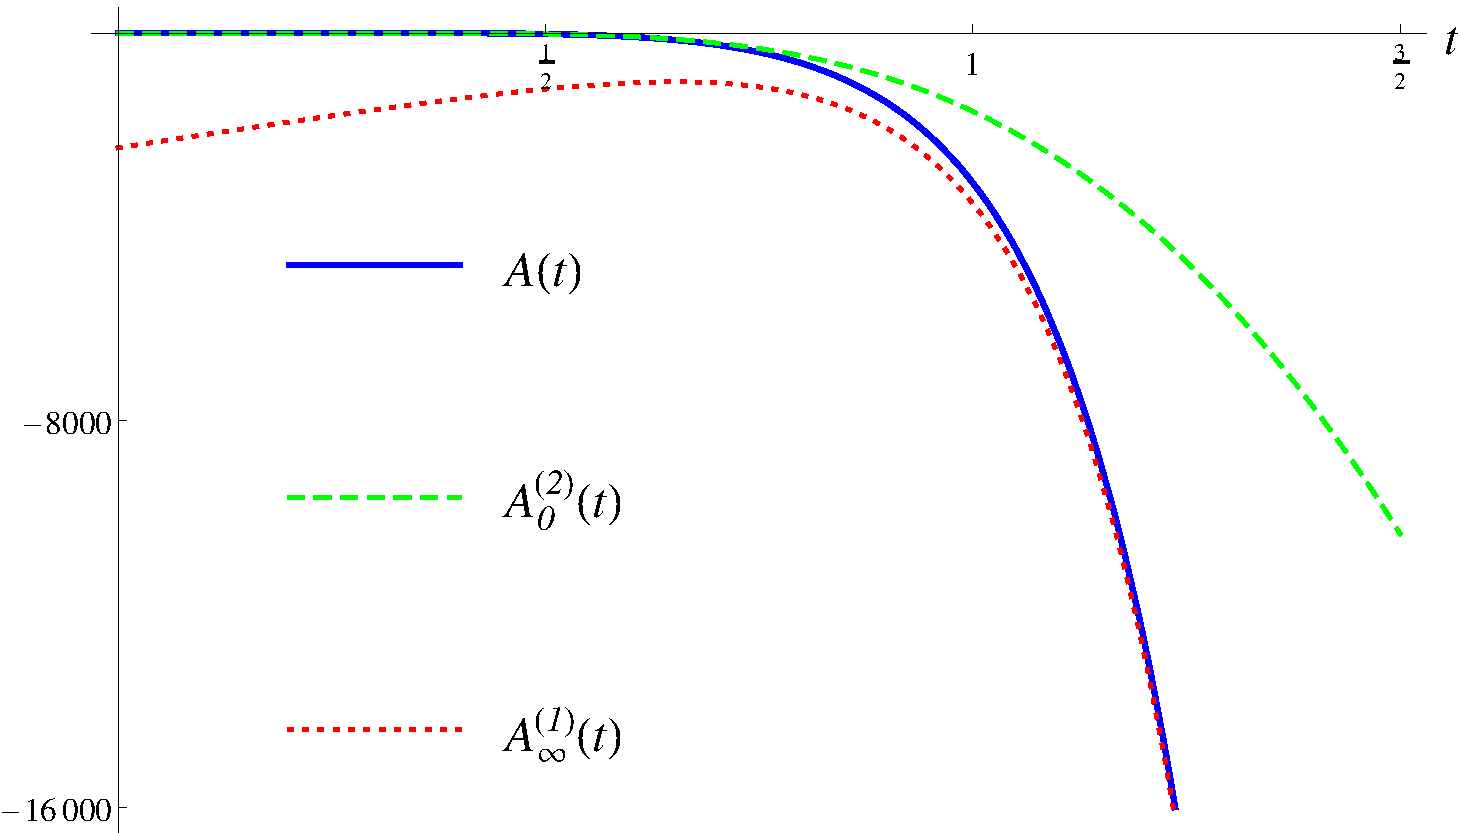
\includegraphics[width=300 pt]{graphics/e8plot_A.pdf}
\end{figure}

\noindent We observe that we can compute the values of $A(t)$ for $t\in(0,\infty)$ with any given precision. Indeed, from identities \eqref{eqn: phi0 transform} and \eqref{eqn: psi S define} we obtain the following two presentations for $A(t)$
\begin{align}
  A(t)=&-t^2\phi_0(i/t)+\frac{36}{\pi^2}\,t^2\,\psi_S(i/t)\notag\\
  A(t)=&-t^2\phi_0(it)+\frac{12}{\pi}\,t\,\phi_{-2}(it)-\frac{36}{\pi^2}\,\phi_{-4}(it)-\frac{36}{\pi^2}\,\psi_I(i/t).\notag
\end{align}
For an integer $n\geq0$ let $A_0^{(n)}$ and  $A_{\infty}^{(n)}$ be the functions such that
\begin{align}
  A(t)=&A_0^{(n)}(t)+O(t^2\,e^{-\pi n /t})\quad\mbox{as}\;t\to0\label{eqn: A asymptotic expansion 0}\\
  A(t)=&A_\infty^{(n)}(t)+O(t^2\,e^{-\pi n t})\quad\mbox{as}\;t\to\infty.\label{eqn: A asymptotic expansion infty}
\end{align}
For each $n\geq 0$ we can compute these functions from the Fourier expansions \eqref{eqn: phi fourier0}--\eqref{eqn: phi fourier4}, \eqref{eqn: psi fourier I}, and \eqref{eqn: psi fourier S}.
  For example, from \eqref{eqn: phi fourier4}--\eqref{eqn: phi fourier0} and \eqref{eqn: psi fourier I} we compute
%$$A_\infty^{(0)}(t)=-\frac{72}{\pi^2}\,e^{2\pi t}$$ and
\begin{align}A_\infty^{(6)}(t)=&\scriptstyle-\tfrac{72}{\pi ^2}\, e^{2 \pi  t}-\tfrac{23328}{\pi ^2}+\tfrac{184320}{\pi ^2}\, e^{-\pi  t}-\tfrac{5194368}{\pi ^2}\, e^{-2 \pi  t}+\tfrac{22560768}{\pi ^2}\, e^{-3 \pi  t}-\tfrac{250583040}{\pi
    ^2}\, e^{-4 \pi  t}+\tfrac{869916672 }{\pi ^2}\,e^{-5 \pi  t}\notag\\&\scriptstyle+t(\tfrac{8640}{\pi }+\tfrac{2436480}{\pi }\, e^{-2 \pi  t}+\tfrac{113011200 }{\pi }\,e^{-4 \pi  t})-t^2(518400\,e^{-2 \pi  t}+31104000\,e^{-4 \pi  t}).\notag
\end{align}
From \eqref{eqn: phi fourier4}--\eqref{eqn: phi fourier0} and \eqref{eqn: psi fourier S} we compute
%$$A_0^{(2)}(t)=-\frac{368640}{\pi^2}\,t^2\,e^{-\pi /t}$$and
$$A_0^{(6)}(t)=t^2(-\tfrac{368640}{\pi ^2}\, e^{-\pi/t}-518400\, e^{-2\pi/t}-\tfrac{45121536}{\pi ^2}\, e^{-3\pi/t}-31104000\,e^{-4\pi/t}-\tfrac{1739833344}{\pi ^2}\, e^{-5\pi/t}).$$
Moreover, from the convergent asymptotic expansion for the Fourier coefficients of a weakly holomorphic modular form \cite[Proposition 1.12]{Bruinier} we find that the $n$-th Fourier coefficient $c_{\psi_I}(n)$ of $\psi_I$ satisfies
\begin{equation}\label{eqn: Fourier estimate 1}|c_{\psi_I}(n)|\leq e^{4\pi\sqrt{n}}\qquad n\in\tfrac 12 \Z_{>0}.\end{equation} Similar inequalities hold for the Fourier coefficients of $\psi_S$, $\phi_0$, $\phi_{-2}$, and $\phi_{-4}$:
\begin{align}\label{eqn: Fourier estimate 2}
&|c_{\psi_S}(n)|\leq 2e^{4\pi\sqrt{n}}\qquad n\in\tfrac 12 \Z_{>0} \\
&|c_{\phi_0}(n)|\leq 2e^{4\pi\sqrt{n}}\qquad n\in \Z_{>0} \\
&|c_{\phi_{-2}}(n)|\leq e^{4\pi\sqrt{n}}\qquad n\in  \Z_{>0} \\
&|c_{\phi_{-4}}(n)|\leq e^{4\pi\sqrt{n}}\qquad n\in \Z_{>0}. \label{eqn: Fourier estimate 5}
  \end{align}
Therefore, we can estimate the error terms in the asymptotic expansions \eqref{eqn: A asymptotic expansion 0} and \eqref{eqn: A asymptotic expansion infty} of $A(t)$
\begin{align}
\left|A(t)-A_0^{(m)}(t)\right|\leq& (t^2+\frac{36}{\pi^2})\,\sum_{n=m}^\infty 2e^{2\sqrt{2}\pi\sqrt{n}}\,e^{-\pi n/t}\notag\\
\left|A(t)-A_\infty^{(m)}(t)\right|\leq& (t^2+\frac{12}{\pi}\,t+\frac{36}{\pi^2})\,\sum_{n=m}^\infty 2e^{2\sqrt{2}\pi\sqrt{n}}\,e^{-\pi nt}.\notag
\end{align}
  For an integer $m\geq0$ we set
\begin{align}
R^{(m)}_0:=&(t^2+\frac{36}{\pi^2})\,\sum_{n=m}^\infty 2e^{2\sqrt{2}\pi\sqrt{n}}\,e^{-\pi n/t}\notag\\
R^{(m)}_\infty:=&(t^2+\frac{12}{\pi}\,t+\frac{36}{\pi^2})\,\sum_{n=m}^\infty 2e^{2\sqrt{2}\pi\sqrt{n}}\,e^{-\pi nt}.\notag
\end{align}
Using interval arithmetic we check that
\begin{align}
&\left|R_0^{(6)}(t)\right|\leq\left|A_0^{(6)}(t)\right|\quad\mbox{ for }\;t\in(0,1]\notag\\
&\left|R_\infty^{(6)}(t)\right|\leq\left|A_\infty^{(6)}(t)\right|\quad\mbox{ for }\;t\in[1,\infty)\notag\\
&A_0^{(6)}(t)<0\quad\mbox{ for }\;t\in(0,1]\notag\\
&A_\infty^{(6)}(t)<0\quad\mbox{ for }\;t\in[1,\infty).\notag
\end{align}
Thus, we see that $A(t)<0$ for $t\in (0,\infty)$. Then identity \eqref{eqn: g A} implies \eqref{eqn: g1}.


Next, we prove \eqref{eqn: g2}. By Propositions~\ref{prop: a another integral} and~\ref{prop: b another integral} we know that for $r>0$
\begin{equation}\label{eqn: g B} \widehat{g}(r)=\frac{\pi}{2160}\,\sin(\pi r^2/2)^2\,\int\limits_0^\infty B(t)\,e^{-\pi r^2 t}\,dt\end{equation}
where $$B(t)=-t^2\phi_0(i/t)+\frac{36}{\pi^2}\,\psi_I(it).$$
This function can be also written as
\begin{align}
  B(t)=&-t^2\phi_0(i/t)-\frac{36}{\pi^2}\,t^2\,\psi_S(i/t)\notag\\
  B(t)=&-t^2\phi_0(it)+\frac{12}{\pi}\,t\,\phi_{-2}(it)-\frac{36}{\pi^2}\,\phi_{-4}(it)+\frac{36}{\pi^2}\,\psi_I(i/t).\notag
\end{align}
Our aim is to prove that $B(t)>0$ for $t\in(0,\infty)$. A plot of $B(t)$ is given in Figure~\ref{fig:B}.
\begin{figure}[h!]
\caption{Plot of the functions $B(t)$, $B^{(2)}_0(t)=\frac{368640}{\pi^2}\,t^2\,e^{-\pi /t}$, and $B^{(1)}_\infty(t)=\frac{8640}{\pi}t-\frac{23328}{\pi^2}$.\label{fig:B}}
  \centering
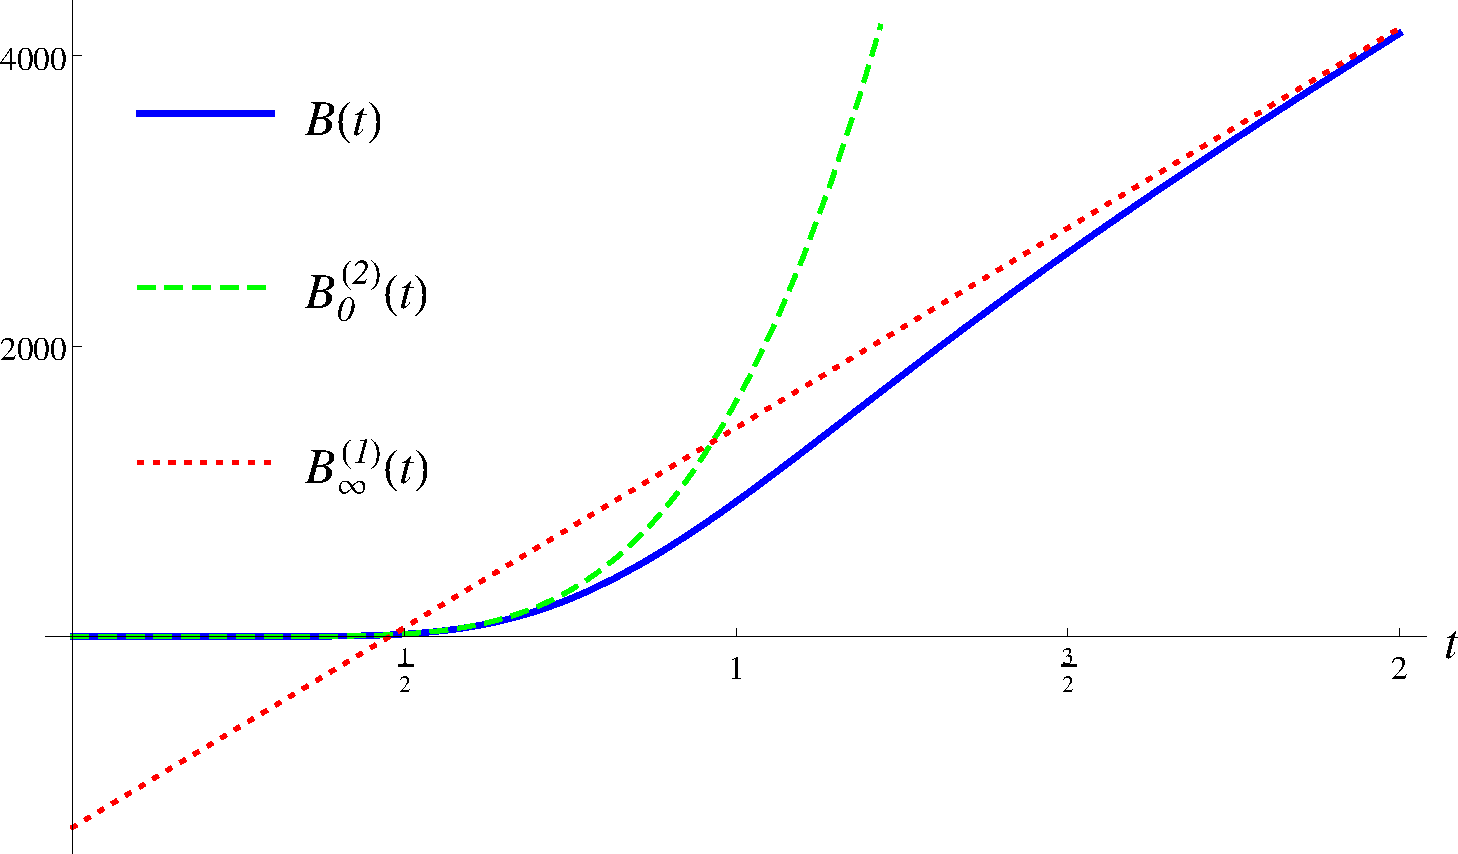
\includegraphics[width=300 pt]{graphics/e8plot_B.pdf}
\end{figure}

\noindent For $n\geq 0$ let $B_0^{(n)}$ and  $B_{\infty}^{(n)}$ be the functions  such that
\begin{align}
  B(t)=&B_0^{(n)}(t)+O(t^2\,e^{-\pi n /t})\quad\mbox{as}\;t\to0\notag\\
  B(t)=&B_\infty^{(n)}(t)+O(t^2\,e^{-\pi n t})\quad\mbox{as}\;t\to\infty.\notag
\end{align}
We find
\begin{align}B_\infty^{(6)}(t)=&-\tfrac{12960}{\pi ^2}-\tfrac{184320}{\pi ^2}\,\scriptstyle e^{-\pi  t}\displaystyle-\tfrac{116640}{\pi ^2} \,\scriptstyle e^{-2\pi  t}\displaystyle-\tfrac{22560768}{\pi ^2}\,\scriptstyle e^{-3\pi  t}\displaystyle+\tfrac{56540160}{\pi ^2}\,\scriptstyle e^{-4\pi  t}\displaystyle-\tfrac{869916672 }{\pi ^2} \,\scriptstyle e^{-5\pi  t}\displaystyle\notag\\
&+t(\tfrac{8640 }{\pi }+\tfrac{2436480}{\pi }\,\scriptstyle e^{-2\pi  t}\displaystyle+\tfrac{113011200 }{\pi }\,\scriptstyle e^{-4\pi  t}\textstyle)-t^2(\scriptstyle518400\,\scriptstyle e^{-2\pi  t}\displaystyle+\scriptstyle31104000\,\scriptstyle e^{-4\pi  t}\displaystyle)\notag
\end{align}
and
$$B_0^{(6)}(t)= t^2(\tfrac{368640}{\pi ^2}\, e^{-\pi/t}-518400\, e^{-2 \pi /t}+\tfrac{45121536 }{\pi ^2}\,e^{-3 \pi/t}-31104000\, e^{-4 \pi/t}+\tfrac{1739833344 }{\pi ^2}\,e^{-5 \pi/t}) .$$
The estimates \eqref{eqn: Fourier estimate 1}--\eqref{eqn: Fourier estimate 5} imply that $$\left|B(t)-B_0^{(6)}(t)\right|\leq R_0^{(6)}(t)\quad\mbox{for}\;t\in(0,1]$$
and
$$\left|B(t)-B_\infty^{(6)}(t)\right|\leq R_\infty^{(6)}(t)\quad\mbox{for}\;t\in[1,\infty).$$
Using interval arithmetic we verify that
\begin{align}
&\left|R_0^{(6)}(t)\right|\leq\left|B_0^{(6)}(t)\right|\quad\mbox{ for }\;t\in(0,1]\notag \\
&\left|R_\infty^{(6)}(t)\right|\leq\left|B_\infty^{(6)}(t)\right|\quad\mbox{ for }\;t\in[1,\infty)\notag \\
&B_0^{(6)}(t)>0\quad\mbox{ for }\;t\in(0,1]\notag \\
&B_\infty^{(6)}(t)>0\quad\mbox{ for }\;t\in[1,\infty). \notag
\end{align}
Now identity \eqref{eqn: g B} implies \eqref{eqn: g2}.

Finally, the property \eqref{eqn: g3} readily follows from Proposition~\ref{prop: a values} and Proposition~\ref{prop: b values}.
This finishes the proof of Theorems~\ref{thm: g1} and~\ref{thm: g}.
  \end{proof}




\begin{thebibliography}{10}
\bibitem{Abramowitz} {\sc M. Abramowitz, I. Stegun}, \emph{ Handbook of Mathematical Functions with Formulas, Graphs, and Mathematical Tables}, Applied Mathematics Series 55 (10 ed.), New York, USA: United States Department of Commerce, National Bureau of Standards; Dover Publications, 1964.

%\bibitem{BRV} {\sc A. Bondarenko, D. Radchenko, M. Viazovska}, \emph{On optimal asymptotic bounds for spherical designs}, Annals of Math. 178 (2)(2013), pp. 443--452.

\bibitem{Bruinier} {\sc J. Bruinier}, \emph{Borcherds products on O(2,l) and Chern classes of Heegner divisors}, Springer Lecture Notes in Mathematics 1780 (2002)

\bibitem{ElkiesCohn}  {\sc H. Cohn, N. Elkies}, \emph{New upper bounds on sphere packings I}, Annals of Math. 157 (2003) pp. 689--714.

%\bibitem{Cohn} {\sc H. Cohn}, \emph{New upper bounds on sphere packings. II.} Geom. Topol. 6 (2002), pp. 329--353.

%\bibitem{CohnKumar} {\sc H. Cohn, A. Kumar}, \emph{Universally optimal distribution of points on spheres}, J. Amer. Math. Soc. 20 (1) (2007), pp. 99--148.

%\bibitem{ConwaySloan}  {\sc J. H. Conway and N. J. A. Sloane}, \emph{What Are All the Best Sphere Packings in Low Dimensions? ,} Discrete Comput. Geom. (Laszlo Fejes Toth Festschrift), 13 (1995), pp. 383--403.


%\bibitem{DukeImamogluToth} {\sc W. Duke, O. Imamoglu and A. Toth}, {\em Cycle integrals of the j-function and mock modular forms}, Ann. of Math. (2) 173 (2011), no. 2, 947-981.

%\bibitem{Deligne1} {\sc P. Deligne}, \emph{Travaux de Shimura.} S\'eminaire Bourbaki, 23\'eme ann\'ee (1970/71), Exp. No. 389, pp. 123-165. Lecture Notes in Math., Vol. 244, Springer, Berlin, 1971.

%\bibitem{Deligne2} {\sc P. Deligne}, \emph{Vari\'et\'es de Shimura: interpr\'etation modulaire, et techniques de construction de mod\'eles canoniques}, in Automorphic forms, representations and L-functions, Proc. Sympos. Pure Math., XXXIII (Corvallis, OR, 1977), Part 2, pp. 247-289, Amer. Math. Soc., Providence, R.I., 1979.



%\bibitem{CohnZ} {\sc H. Cohn, Y. Zhao}, \emph{Sphere packing bounds via spherical codes}, arXiv:1212.5966 [math.MG]

%\bibitem{Delsarte72} {\sc P. Delsarte},\emph{Bounds for unrestricted codes, by linear programming}, Philips Res. Rep. 27 (1972), pp. 272--289.


%\bibitem{Delsarte77} {\sc P. Delsarte, J. M. Goethals, and J. J. Seidel}, \emph{Spherical codes and designs}, Geom. Dedicata, 6 (1977), pp. 363--388.

\bibitem{first course} {\sc F. Diamond, J. Shurman}, \emph{A First Course in Modular Forms}, Springer New York, 2005.

%\bibitem{Toth} {\sc L. Fejes Toth}, {\em {\"U}ber die dichteste Kugellagerung}, Math. Z. 48 (1943), pp. 676--684.

%\bibitem{Hales} {\sc T. Hales}, {\em A proof of the Kepler conjecture}, Annals of Math. 162 (3) (2005), pp. 1065--1185.

\bibitem{Hejhal} {\sc D. Hejhal}, {\em The Selberg trace formula for $\mathrm{PSL}(2, \R)$},  Springer Lecture Notes in Mathematics 1001 (1983)

%\bibitem{KabLev} {\sc G. A. Kabatiansky and V. I. Levenshtein}, {\em Bounds for packings on a sphere and in space},Problems of Information Transmission 14 (1978), pp. 1--17.

\bibitem{Mumford} {\sc D. Mumford}, {\em Tata Lectures on Theta I}, Birkh\"auser, 1983.

%\bibitem{Ma} {\sc Manin, Yu. I.}, {\em Real multiplication and noncommutative geometry (ein Alterstraum)}. The legacy of Niels Henrik Abel, 685-727, Springer, Berlin, 2004.

%\bibitem{MaOdSl} {\sc C. L. Mallows, A. M. Odlyzko, and N. J. A. Sloane}, {\em Upper bounds for modular forms, lattices, and codes}, J. Algebra, 36 (1975), 68--76

\bibitem{Petersson32} {\sc H. Petersson}, {\em Ueber die Entwicklungskoeffizienten der automorphen Formen}, Acta Mathematica, Bd. 58 (1932),  pp. 169--215.

%\bibitem{PfenderZiegler} {\sc F. Pfender, G. M. Ziegler,} {\em Kissing numbers, sphere packings, and some unexpected proofs}, Notice of the AMS  51 (8) (2004) pp. 873--883

\bibitem{Rademacher38} {\sc H. Rademacher and H. S. Zuckerman}, {\em On the Fourier coefficients of certain modular forms of
positive dimension}, Annals of Math. (2) 39 (1938),  pp. 433--462.

%\bibitem{Thue} {\sc A. Thue}, {\em {\"U}ber die dichteste Zusammenstellung von kongruenten Kreisen in einer Ebene}, Norske Vid. Selsk. Skr. No.1 (1910), pp. 1--9.

%\bibitem{Venk}   {\sc  A. Venkatesh}, {\em A Note on Sphere Packings in High Dimension}, International Mathematics Research Notices  7 (2013),  1628--1642

%\bibitem{Yudin} {\sc V. A. Yudin}, {\em Lower bounds for spherical designs}, Izv. Ross. Akad. Nauk. Ser. Mat. 61 (1997), pp. 211-233. English transl., Izv. Math. 6 (1997), pp. 673--683.

\bibitem{1-2-3} {\sc D. Zagier}, {\em Elliptic Modular Forms and Their Applications}, In:  The 1-2-3 of Modular Forms, (K. Ranestad, ed.) Norway, Springer Universitext, 2008.
\end{thebibliography}

\newpage

{\footnotesize
\noindent
Ecole Polytechnique Federale de Lausanne\\
1015 Lausanne\\
Switzerland\\
{\it Email address: maryna.viazovska@epfl.ch}}

\end{document}


\title{Sphere Packing in Lean}
\author{Maryna Viazovska}

\begin{document}
\maketitle
% In this file you should put the actual content of the blueprint.
% It will be used both by the web and the print version.
% It should *not* include the \begin{document}
%
% If you want to split the blueprint content into several files then
% the current file can be a simple sequence of \input. Otherwise It
% can start with a \section or \chapter for instance.

\begin{abstract}
  In this paper we prove that no packing of unit balls in Euclidean space $\R^8$ has density greater than that of the $E_8$-lattice packing.
  \ifplastex
  % web
  The PDF version of this blueprint is available \href{https://thefundamentaltheor3m.github.io/Sphere-Packing-Lean/blueprint.pdf}{here}.
  \else
  % print
  The web version of this blueprint is available \href{https://thefundamentaltheor3m.github.io/Sphere-Packing-Lean/blueprint/index.html}{here}.
  \fi
  \end{abstract}


\section{Basic definitions for sphere packings}
\subsection{Sphere packings}
The sphere packing constant measures which portion of $d$-dimensional Euclidean
space can be covered by non-overlapping unit balls. More precisely, let $\R^d$ be the Euclidean vector space equipped with distance $\|\cdot\|$ and Lebesgue measure $\mathrm{Vol}(\cdot)$. For $x\in\R^d$ and $r\in\R_{>0}$ we denote by $B_d(x,r)$ the ball in $\R^d$ with center $x$ and radius $r$.

\begin{definition}\label{SpherePacking.isPacking}\lean{SpherePacking.isPacking}\leanok
  Let $X\subset \R^d$ be a discrete set of points such that $\|x-y\|\geq2$ for any distinct $x,y\in X$. Then the union
$$\mathcal{P}=\bigcup_{x\in X} B_d(x,1)$$ is a \emph{sphere packing}.
\end{definition}

\begin{definition}\label{SpherePacking.isLatticePacking}\uses{EuclideanLattice.is_lattice}\lean{SpherePacking.isLatticePacking}\leanok
  If $X$ is a lattice in $\R^d$ then we say that $\mathcal{P}$ is a \emph{lattice sphere packing}.
\end{definition}

\begin{definition}\label{SpherePacking.FiniteDensity}\lean{SpherePacking.FiniteDensity}\leanok
  The \emph{finite density} of a packing $\mathcal{P}$ is defined as
$$\Delta_{\mathcal{P}}(r):=\frac{\mathrm{Vol}(\mathcal{P}\cap B_d(0,r))}{\mathrm{Vol}(B_d(0,r))},\quad r>0.$$
\end{definition}

\begin{definition}\label{SpherePacking.Density}\uses{SpherePacking.FiniteDensity}\lean{SpherePacking.Density}\leanok
  We define the \emph{density} of a packing $\mathcal{P}$ as the limit superior
$$\Delta_{\mathcal{P}}:=\limsup\limits_{r\to\infty}\Delta_{\mathcal{P}}(r). $$
\end{definition}

\begin{definition}\label{SpherePacking.Constant}\uses{SpherePacking.isPacking, SpherePacking.Density}\lean{SpherePacking.Constant}\leanok
The number be want to know is the supremum over all possible packing densities
$$\Delta_d:=\sup\limits_{\substack{\mathcal{P}\subset\R^d\\ \scriptscriptstyle\mathrm{sphere}\;\mathrm{packing}}}\Delta_{\mathcal{P}} $$
called the \emph{sphere packing constant}.
\end{definition}

The main result of this paper is the proof that $$\Delta_8=\frac{\pi^4}{384}\approx 0.25367.$$
This is the density of the $E_8$-lattice sphere packing.

\begin{definition}\label{EuclideanLattice.E8}\lean{EuclideanLattice.E8}
  Recall that the $E_8$-lattice $\Lambda_8\subset\R^8$ is given by
$$\Lambda_8=\{(x_i)\in\Z^8\cup(\Z+\textstyle\frac12\displaystyle )^8|\;\sum_{i=1}^8x_i\equiv 0\;(\mathrm{mod\;2})\}.$$
\end{definition}
\begin{lemma}\label{lemma: Characterisation of E8 lattice}
  $\Lambda_8$ is a positive-definite, even, unimodular lattice of rank 8. The minimal distance between two points in $\Lambda_8$ is $\sqrt{2}$.
\end{lemma}
\begin{definition}\label{SpherePacking.E8}\uses{EuclideanLattice.E8}\lean{SpherePacking.E8}\leanok
The $E_8$-lattice sphere packing is the packing of unit balls with centers at $\frac{1}{\sqrt{2}}\Lambda_8$.
\end{definition}
Our main result is
\begin{theorem}\label{SpherePacking.Main}\lean{SpherePacking.Main}
No packing of unit balls
in Euclidean space $\R^8$ has density greater than that of the $E_8$-lattice packing.
\end{theorem}

\subsection{Lattices and Periodic packings}
\begin{definition}\label{def: Periodicity}
  Let $S$ be a discrete subgroup of $\R^d$. A set $X\subset\R^d$ is said to $S$-periodic if for each $s\in S$ and $x\in X$ the vector $x+s$ belongs to $X$.
\end{definition}

\begin{definition}\label{EuclideanLattice.is_lattice}\lean{EuclideanLattice.is_lattice}\leanok
  % A lattice in the Euclidean space $\R^d$ is a discrete, co-compact, abelian subgroup.
  A subset of the Euclidean space $\R^d$ is called a lattice if it is the $\Z$-span of a basis of $\R^d$.
\end{definition}

\begin{lemma}\label{SpherePacking.Density of periodic packing} \notready
  Density of a periodic packing ...
\end{lemma}
\subsection{Facts from Fourier analysis}
hello
In this subsection we recall a few definitions from Fourier analysis.
\begin{definition}\label{def: Fourier Transform definition} % \lean{def: Fourier Transform definition}
The Fourier transform of an $L^1$-function $f:\R^d\to\C$ is defined as
$$\mathcal{F}(f)(y)=\widehat{f}(y):=\int\limits_{\R^d} f(x)\,e^{-2\pi i x\cdot y}\,dx,\quad y\in\R^d $$
where $x\cdot y=\frac12\|x\|^2+\frac12\|y\|^2-\frac12\|x-y\|^2$ is the standard scalar product in $\R^d$.
\end{definition}
\begin{definition}
A $C^\infty$~function $f:\R^d\to\C$ is called a \emph{Schwartz function} if it goes to zero as $\|x\|\to\infty$ faster then any inverse power of $\|x\|$, and the same holds for all partial derivatives of $f$. The set of all Schwartz functions is called a \emph{Schwartz space}.
\end{definition}
\begin{lemma}\label{lemma: Fourier transform is automorphism}
  The Fourier transform is an automorphism of the space of Schwartz functions.
\end{lemma}
\begin{lemma}\label{lemma: Gaussian Fourier}\uses{def: Fourier Transform definition}
\begin{equation}\mathcal{F}(e^{\pi i  \|x\|^2 z})(y)=z^{-4}\,e^{\pi i \|y\|^2 \,(\frac{-1}{z}) }.\end{equation}
\end{lemma}
\begin{theorem}\label{thm: Poisson summation formula}\uses{def: Fourier Transform definition}
  (Poisson summation formula)$$\sum_{\ell\in\Lambda}f(\ell)=\frac{1}{\mathrm{vol}(\R^d/\Lambda)}\sum_{m\in\Lambda^*}\widehat{f}(m).$$
\end{theorem}

\section{Cohn-Elkies linear programming bounds}

In 2003 Cohn and Elkies \cite{ElkiesCohn}  developed  linear programming bounds that apply directly to sphere packings. The goal of this section is to formalize the Cohn--Elkies linear programming bound.

The following theorem is the key result of \cite{ElkiesCohn}. (The original theorem is stated for a   class of functions more general then Schwartz functions)
\begin{theorem}\label{thm: Cohn-Elkies}\uses{def: Fourier Transform definition}\uses{thm: Poisson summation formula}
(Cohn, Elkies \cite{ElkiesCohn}) Suppose that  $f:\R^d\to\R$ is a Schwartz function, is not identically zero, and satisfies:
\begin{equation}\label{eqn: Cohn-Elkies condition 1}f(x)\leq 0\mbox{ for } \|x\|\geq 1\end{equation} and
\begin{equation}\label{eqn: Cohn-Elkies condition 2}\widehat{f}(x)\geq0\mbox{ for all } x\in\R^d.\end{equation}
  Then the  density of  $d$-dimensional
  sphere packings is bounded above by $$\frac{f(0)}{\widehat{f}(0)}\cdot \frac{\pi^{\frac{d}{2}}}{2^d\,\Gamma(\textstyle \frac{d}{2}+1)}.$$
\end{theorem}
\begin{proof}
To be included.
\end{proof}


  The main step in our proof of Theorem \ref{SpherePacking.Main} is the explicit  construction of an optimal function. It will be convenient for us to scale this function by $\sqrt{2}$.
\begin{theorem}\label{thm: g}
There exists a radial Schwartz function $g:\R^8\to\R$ which satisfies:
\begin{align}
g(x)&\leq 0\mbox{ for } \|x\|\geq \sqrt{2} \label{eqn: g1}\\
\widehat{g}(x)&\geq0\mbox{ for all } x\in\R^8\label{eqn: g2}\\
g(0)&=\widehat{g}(0)=1.\label{eqn: g3}
\end{align}
\end{theorem}
Theorem \ref{thm: Cohn-Elkies} applied to the optimal function $f(x)=g(x/\sqrt{2})$ immediately implies Theorem \ref{SpherePacking.Main}.


\section{Modular forms}
Let $\h$ be the upper half-plane $\{z\in\C\mid\Im(z)>0\}$. The modular group $\Gamma_1:=\mathrm{PSL}_2(\Z)$ acts on $\h$ by linear fractional transformations
$$\left(\begin{smallmatrix}a&b\\c&d\end{smallmatrix}\right)z:=\frac{az+b}{cz+d}.$$

Let $N$ be a positive integer. The \emph{level $N$ principal congruence subgroup} of $\Gamma_1$ is
$$\Gamma(N):=\left\{\left.\left(\begin{smallmatrix}a&b\\c&d\end{smallmatrix}\right)\in\Gamma_1\right|\left(\begin{smallmatrix}a&b\\c&d\end{smallmatrix}\right)\equiv\left(\begin{smallmatrix}1&0\\0&1\end{smallmatrix}\right)\;\mathrm{mod}\;N\right\}.$$
A subgroup $\Gamma\subset\Gamma_1$ is called a \emph{congruence subgroup} if $\Gamma(N)\subset\Gamma$ for some $N\in\N$. An important example of a congruence subgroup is
$$\Gamma_0(N):=\left\{\left.\left(\begin{smallmatrix}a&b\\c&d\end{smallmatrix}\right)\in\Gamma_1\right|\;c\equiv0\;\mathrm{mod}\;N\right\}.$$

Let $z\in\h$, $k\in\Z$, and $\left(\begin{smallmatrix}a&b\\c&d\end{smallmatrix}\right)\in\mathrm{SL}_2(\Z)$. The \emph{automorphy factor} of weight $k$ is defined as
$$j_k(z,\left(\begin{smallmatrix}a&b\\c&d\end{smallmatrix}\right)):=(cz+d)^{-k}.$$
The automorphy factor satisfies the \emph{chain rule}
$$j_k(z,\gamma_1\gamma_2)=j_k(z,\gamma_1)\,j_k(\gamma_2z,\gamma_1). $$
Let $F$ be a  function on $\h$ and $\gamma\in\mathrm{PSL}_2(\Z)$. Then the \emph{slash operator} acts on $F$ by
$$(F|_k\gamma)(z):=j_k(z,\gamma)\,F(\gamma z). $$
The chain rule implies
$$F|_k\gamma_1\gamma_2=(F|_k\gamma_1)|_k\gamma_2.$$

\begin{definition}\label{def: holomorphic modular form}% \lean{def: holomorphic modular form}
A \emph{(holomorphic) modular form} of integer weight $k$ and congruence subgroup $\Gamma$ is a holomorphic function $f:\h\to\C$ such that:
\begin{enumerate}
  \item $f|_k\gamma=f$ for all $\gamma\in\Gamma$
  \item for each $\alpha\in\Gamma_1\;f|_k\alpha$ has the Fourier expansion $f|_k\alpha (z)=\sum_{n=0}^\infty c_f(\alpha,\frac{n}{n_\alpha})\,e^{2\pi i \frac{n}{n_\alpha}z}$ for some $n_\alpha\in\N$ and Fourier coefficients $c_f(\alpha,m)\in\C$.
\end{enumerate}
\end{definition}

Let $M_k(\Gamma)$ be the space of modular forms of weight $k$ and congruence subgroup $\Gamma$. A key fact in the theory of modular forms is that the spaces $M_k(\Gamma)$ are finite dimensional.

Let us consider several examples of modular forms.
\begin{definition}\label{def: Ek definition}% \lean{def: Ek definition}
For an even integer $k\geq 4$ we define the \emph{weight $k$ Eisenstein series} as
\begin{equation}\label{eqn: Ek definition}E_k(z):=\frac{1}{2\zeta(k)}\sum_{(c,d)\in\Z^2\backslash(0,0)}(c\tau+d)^{-k}.\end{equation}
\end{definition}
Since the sum converges absolutely, it is easy to see that $E_k\in M_k(\Gamma_1)$.
\begin{lemma}\label{lemma: Ek Fourier}
% \lean{lemma: Ek Fourier}\uses{def: Ek definition}
The Eisenstein series possesses the Fourier expansion
\begin{equation}\label{eqn: Ek Fourier}E_k(z)=1+\frac{2}{\zeta(1-k)}\sum_{n=1}^\infty \sigma_{k-1}(n)\,e^{2\pi i z}, \end{equation}
where $\sigma_{k-1}(n)\,=\,\sum_{d|n} d^{k-1}$. In particular, we have
\begin{align}
  E_4(z)\,=\,& 1+240\sum_{n=1}^\infty \sigma_3(n)\,e^{2\pi i n z} \notag \\
  E_6(z)\,=\,& 1-504\sum_{n=1}^\infty \sigma_5(n)\,e^{2\pi i n z}. \notag
\end{align}
\end{lemma}
The infinite sum \eqref{eqn: Ek definition} does not converge absolutely for $k=2$. On the other hand, the expression \eqref{eqn: Ek Fourier} converges to a holomorphic function on the upper half-plane and therefore
\begin{definition} \label{def: E2 def} % \lean{def: E2 def}
We set
\begin{equation}E_2(z):= 1-24\sum_{n=1}^\infty \sigma_1(n)\,e^{2\pi i n z}.\notag\end{equation}
\end{definition}
\begin{lemma}
\label{lemma: E2 transform}

% \lean{lemma: Ek Fourier}

This function is not modular, however it satisfies
\begin{equation}\label{eqn: E2 transform}z^{-2}\,E_2\Big(\frac{-1}{z}\Big)=E_2(z) -\frac{6i}{\pi}\, \frac{1}{z}.\end{equation}
\end{lemma}
The proof of this identity can be found in \cite[Section~2.3]{1-2-3}.
The weight two Eisenstein series $E_2$ is an example of a \emph{quasimodular form} \cite[Section~5.1]{1-2-3}.

Another example of modular forms we would like to consider are \emph{theta functions} \cite[Section~3.1]{1-2-3}.
We define three different theta functions (so called ``Thetanullwerte'') as
\begin{align}
  \theta_{00}(z)\,=\, & \sum_{n\in\Z}e^{\pi i n^2 z} \notag \\
  \theta_{01}(z)\,=\, & \sum_{n\in\Z}(-1)^n\,e^{\pi i n^2 z} \notag \\
  \theta_{10}(z)\,=\, & \sum_{n\in\Z}e^{\pi i (n+\frac12)^2 z}. \notag
\end{align}
The group $\Gamma_1$ is generated by the elements $T=\left(\begin{smallmatrix}1&1\\0&1\end{smallmatrix}\right)$ and $S=\left(\begin{smallmatrix}0&1\\-1&0\end{smallmatrix}\right)$.
\begin{lemma}\label{lemma: theta transform S T}
% \lean{lemma: theta transform S T}

These elements  act on the theta functions in the following way
\begin{align}
z^{-2}\,\theta^4_{00}\Big(\frac{-1}{z}\Big)\,=\,&-\theta_{00}^4(z) \label{eqn: theta transform S}\\
z^{-2}\,\theta^4_{01}\Big(\frac{-1}{z}\Big)\,=\,&-\theta_{10}^4(z)\\
z^{-2}\,\theta^4_{10}\Big(\frac{-1}{z}\Big)\,=\,&-\theta_{01}^4(z)
\end{align}
and
\begin{align}
\theta^4_{00}(z+1)\,=\,&\theta_{01}^4(z)\\
\theta^4_{01}(z+1)\,=\,&\theta_{00}^4(z)\\
\theta^4_{10}(z+1)\,=\,&-\theta_{10}^4(z). \label{eqn: theta transform T}
\end{align}
\end{lemma}
Moreover, these three theta functions satisfy the \emph{Jacobi identity}
\begin{equation}
\theta_{01}^4+\theta_{10}^4=\theta_{00}^4.
\end{equation}
The theta functions $\theta^4_{00},\theta^4_{01}$, and $\theta^4_{10}$ belong to $M_2(\Gamma(2))$.


\begin{definition}\label{def: weakly-holomorphic modular form}
A \emph{weakly-holomorphic modular form} of integer weight $k$ and congruence subgroup $\Gamma$ is a holomorphic function $f:\h\to\C$ such that:
\begin{enumerate}
  \item $f|_k\gamma=f$ for all $\gamma\in\Gamma$
  \item for each $\alpha\in\Gamma_1\;f|_k\alpha$ has the Fourier expansion $f|_k\alpha (z)=\sum_{n=n_0}^\infty c_f(\alpha,\frac{n}{n_\alpha})\,e^{2\pi i \frac{n}{n_\alpha}z}$ for some $n_0\in\Z$ and $n_\alpha\in\N$.
\end{enumerate}
\end{definition}
For an $m$-periodic holomorphic function $f$ and $n\in\frac 1m \Z$ we will denote the $n$-th Fourier coefficient of $f$ by $c_f(n)$ so that
$$f(z)=\sum_{n\in\frac 1m \Z} c_f(n)\,e^{2\pi i n z}.$$
We denote the space of weakly-holomorphic modular forms of weight $k$ and group $\Gamma$ by $M_k^!(\Gamma)$. The spaces $M_k^!(\Gamma)$ are infinite dimensional.
Probably the most famous weakly-holomorphic modular form is the \emph{elliptic j-invariant}
$$j\,:=\,\frac{1728\, E_4^3}{E_4^3-E_6^2}. $$
This function belongs to $M_0^!(\Gamma_1)$ and has the Fourier expansion
$$j(z)\,=\,q^{-1} + 744 + 196884\, q + 21493760\, q^2 + 864299970\, q^3 +
  20245856256\, q^4 + O(q^5) $$
  where $q=e^{2\pi i z}$. Using a simple computer algebra system such as PARI GP or Mathematica one can compute first hundred terms of this Fourier expansion within few seconds. An important question is to find an  asymptotic formula for $c_j(n)$, the $n$-th Fourier coefficient  of $j$. Using the Hardy-Ramanujan circle method \cite{Rademacher38} or the non-holomorphic Poincare series \cite{Petersson32} one can show that
  \begin{lemma}\label{lemma: j Fourier asymptotic}
  % \lean{lemma: j Fourier asymptotic}
  \begin{equation}\label{eqn: j Fourier asymptotic}
  c_j(n)=\frac{2\pi}{n}\sum_{k=1}^\infty \frac{A_k(n)}{k}\,I_1\left(\frac{4\pi \sqrt{n}}{k}\right)\qquad n\in\Z_{>0}\end{equation}
  where
  $$A_k(n)= \sum_{\substack{h\;\mathrm{mod}\;k\\(h,k)=1}} e^{\frac{-2\pi i}{k}(nh+h')},\quad hh'\equiv -1(\mbox{mod}\;k),$$
  and $I_\alpha(x)$ denotes the modified Bessel function of the first kind defined as in \cite[Section~9.6]{Abramowitz}.
  \end{lemma}
  A similar convergent asymptotic expansion holds for the Fourier coefficients of any weakly holomorphic modular form \cite{Hejhal}, \cite[Propositions~1.10 and~1.12]{Bruinier}. Such a convergent expansion implies effective estimates for the Fourier coefficients.




\section{Fourier eigenfunctions with double zeroes at lattice points}\label{sec: fourier double zeroes}
In this section we construct two radial Schwartz functions $a,b:\R^8\to i\R$ such that
\begin{align}\mathcal{F}(a)&=a\label{eqn: a fourier}\\
  \mathcal{F}(b)&=-b\label{eqn: b fourier}
\end{align}
which double zeroes at all $\Lambda_8$-vectors of length greater than $\sqrt{2}$. Recall that each vector of $\Lambda_8$ has length $\sqrt{2n}$ for some $n\in\N_{\geq 0}$. We define $a$ and $b$ so that their values are purely imaginary because this simplifies some of our computations. We will show in Section \ref{sec: g} that an appropriate linear combination of functions $a$ and $b$ satisfies conditions \eqref{eqn: g1}--\eqref{eqn: g3}.

First, we will define function $a$. To this end we consider the following functions:
\begin{definition}\label{def: phi4 phi2 phi0}
\uses{def: Ek definition}
\begin{align}
  \phi_{-4}\,:= \,& -Dj\,E_6^{-1}\label{eqn: def phi4}\\
  \phi_{-2}\,:= \,&\phi_{-4}\,E_2+Dj\,E_4^{-1}\label{eqn: def phi2}\\
  \phi_{0}\,:= \,&\phi_{-4}\,E_2^2+2Dj\,E_4^{-1}\,E_2+j-1728.\label{eqn: def phi0}
\end{align}
\end{definition}
Here $Dj(z)=\frac{1}{2\pi i} \frac{d}{dz} j(z)$.
\begin{lemma}\label{lemma: phi fourier4 phi fourier2 phi fourier0}
  These functions have the Fourier expansions
\begin{align}
  \phi_{-4}(z)\,=\,&q^{-1} + 504 + 73764\, q + 2695040\, q^2 + 54755730\, q^3 + O(q^4)\label{eqn: phi fourier4}\\
  \phi_{-2}(z)\,=\,&720 + 203040\, q + 9417600\, q^2 + 223473600\, q^3 + 3566782080\, q^4+O(q^5)\label{eqn: phi fourier2}\\
  \phi_{0}(z)\,=\,&518400\, q + 31104000\, q^2 + 870912000\, q^3 + 15697152000\, q^4+O(q^5)\label{eqn: phi fourier0}
\end{align}
where $q=e^{2\pi i z}$.
\end{lemma}
The function $\phi_0(z)$ is not modular; however,
\begin{lemma}\label{lemma: phi0 transform}
  The identity \ref{lemma: E2 transform} implies the following transformation rule:
\begin{equation}\label{eqn: phi0 transform}
\phi_0\Big(\frac{-1}{z}\Big)=\phi_0(z)-\frac{12i}{\pi}\,\frac{1}{z}\,\phi_{-2}(z)-\frac{36}{\pi^2}\,\frac{1}{z^2}\,\phi_{-4}(z).
\end{equation}
\end{lemma}
\begin{definition}\label{def: a(r) definition}
For $x\in\R^8$ we define
\begin{align}\label{eqn: a(r) definition}
  a(x):=&\int\limits_{-1}^i\phi_0\Big(\frac{-1}{z+1}\Big)\,(z+1)^2\,e^{\pi i \|x\|^2 z}\,dz
  +\int\limits_{1}^i\phi_0\Big(\frac{-1}{z-1}\Big)\,(z-1)^2\,e^{\pi i \|x\|^2 z}\,dz\\
  -&2\int\limits_{0}^i\phi_0\Big(\frac{-1}{z}\Big)\,z^2\,e^{\pi i \|x\|^2 z}\,dz
  +2\int\limits_{i}^{i\infty}\phi_0(z)\,e^{\pi i \|x\|^2 z}\,dz.\nonumber
\end{align}
\end{definition}
We observe that the contour integrals in \eqref{eqn: a(r) definition} converge absolutely and uniformly for  $x\in\R^8$. Indeed,
$\phi_0(z)=O(e^{-2\pi i z})$ as $\Im(z)\to \infty$. Therefore, $a(x)$ is well defined. Now we prove that $a$ satisfies condition \eqref{eqn: a fourier}.
\begin{proposition}\label{prop: a(r) Fourier}\uses{lemma: Ek Fourier}\uses{def: E2 def}\uses{lemma: j Fourier asymptotic}\uses{def: a(r) definition}\uses{lemma: Gaussian Fourier}

The function $a$ defined by \eqref{eqn: a(r) definition} belongs to the Schwartz space and satisfies $$\widehat{a}(x)=a(x). $$
\end{proposition}
\begin{proof}
First, we prove that $a$ is a Schwartz function. From Lemma \ref{lemma: Ek Fourier}, Definition \ref{def: E2 def}, and \ref{lemma: j Fourier asymptotic} we deduce that the Fourier coefficients of $\phi_0$ satisfy
$$|c_{\phi_0}(n)|\leq2\,e^{4\pi\sqrt{n}}\quad n\in\Z_{>0}.$$ Thus, there exists a positive constant $C$ such that
$$|\phi_0(z)|\leq C\,e^{-2\pi \Im{z}}\qquad \mbox{for } \; \Im{z}>\frac 12.$$
We estimate the first summand in the right-hand side of \eqref{eqn: a(r) definition}.  For $r\in\R_{\geq 0}$ we have
\begin{align}&\Bigg|\int\limits_{-1}^{i}\phi_0\Big(\frac{-1}{z+1}\Big)\,(z+1)^2\,e^{\pi i r^2 z}\,dz\Bigg|=\Bigg|\int\limits_{i\infty}^{-1/(i+1)}\phi_0(z)\,z^{-4}\,e^{\pi i r^2 (-1/z-1)}\,dz\Bigg|\leq \notag\\
  &C_1\int\limits_{1/2}^{\infty}e^{-2\pi t}\,e^{-\pi  r^2/t}\,dt\leq C_1\int\limits_{0}^{\infty}e^{-2\pi t}\,e^{-\pi  r^2/t}\,dt=C_2\,r\,K_1(2\sqrt{2}\,\pi\,r)\notag
\end{align}
where $C_1$ and $C_2$ are some positive constants and $K_\alpha(x)$ is the modified Bessel function of the second kind defined as in \cite[Section~9.6]{Abramowitz}. This estimate also holds for the second and third summand in \eqref{eqn: a(r) definition}.
For the last summand we have
$$ \Bigg|\int\limits_{i}^{i\infty}\phi_0(z)\,e^{\pi i r^2 z}\,dz\Bigg|\leq C\,\int\limits_{1}^{\infty} e^{-2\pi t}\,e^{-\pi r^2 t}\,dt=C_3\frac{e^{\pi(r^2+2)}}{r^2+2}.$$
Therefore, we arrive at
$$|a(r)|\leq 4C_2\,r\,K_1(2\sqrt{2}\pi r)+2C_3\frac{e^{-\pi(r^2+2)}}{r^2+2}.$$
It is easy to see that the left hand side of this inequality decays faster then any inverse power of $r$. Analogous estimates can be obtained for all derivatives $\frac{d^k}{dr^k}a(r)$.

Now we show that $a$ is an eigenfunction of the Fourier transform. We recall that the Fourier transform of a Gaussian function is
\begin{equation}\label{eqn: Gaussian Fourier}\mathcal{F}(e^{\pi i  \|x\|^2 z})(y)=z^{-4}\,e^{\pi i \|y\|^2 \,(\frac{-1}{z}) }.\end{equation}
Next, we exchange the contour integration with respect to $z$ variable and Fourier transform  with respect to $x$ variable in \eqref{eqn: a(r) definition}. This can be done, since the corresponding double integral converges absolutely. In this way we obtain
\begin{align}
  \widehat{a}(y)=&\int\limits_{-1}^i\phi_0\Big(\frac{-1}{z+1}\Big)\,(z+1)^2\,z^{-4}\,e^{\pi i \|y\|^2 \,(\frac{-1}{z})}\,dz
  +\int\limits_{1}^i\phi_0\Big(\frac{-1}{z-1}\Big)\,(z-1)^2\,z^{-4}\,e^{\pi i \|y\|^2 \,(\frac{-1}{z})}\,dz\notag \\
  -&2\int\limits_{0}^i\phi_0\Big(\frac{-1}{z}\Big)\,z^2\,z^{-4}\,e^{\pi i \|y\|^2 \,(\frac{-1}{z})}\,dz +2\int\limits_{i}^{i\infty}\phi_0(z)\,z^{-4}\,e^{\pi i \|y\|^2 \,(\frac{-1}{z})}\,dz.\notag
\end{align}
Now we make a change of variables $w=\frac{-1}{z}$. We obtain
\begin{align}
  \widehat{a}(y)=&\int\limits_{1}^i\phi_0\Big(1-\frac{1}{w-1}\Big)\,(\frac{-1}{w}+1)^2\,w^{2}\,e^{\pi i \|y\|^2 \,w}\,dw\notag\\
  +&\int\limits_{-1}^i\phi_0\Big(1-\frac{1}{w+1}\Big)\,(\frac{-1}{w}-1)^2\,w^2\,e^{\pi i \|y\|^2 \,w}\,dw\\
  -&2\int\limits_{i \infty}^i\phi_0(w)\,e^{\pi i \|y\|^2 \,w}\,dw +2\int\limits_{i}^{0}\phi_0\Big(\frac{-1}{w}\Big)\,w^{2}\,e^{\pi i \|y\|^2 \,w}\,dw.\notag
\end{align}
Since $\phi_0$ is $1$-periodic we have
\begin{align}
  \widehat{a}(y)\,=\,&\int\limits_{1}^i\phi_0\Big(\frac{-1}{z-1}\Big)\,(z-1)^2\,e^{\pi i \|y\|^2 \,z}\,dz
  +\int\limits_{-1}^i\phi_0\Big(\frac{-1}{z+1}\Big)\,(z+1)^2\,e^{\pi i \|y\|^2 \,z}\,dz\notag \\
  +&2\int\limits_{i}^{i\infty}\phi_0(z)\,e^{\pi i \|y\|^2 \,z}\,dz
  -2\int\limits_{0}^{i}\phi_0\Big(\frac{-1}{z}\Big)\,z^{2}\,e^{\pi i \|y\|^2 \,z}\,dz\notag \\
  \,=\,&a(y).
\end{align}
This finishes the proof of the proposition.
\end{proof}

Next, we check that $a$ has double zeroes at all $\Lambda_8$-lattice points of length greater then $\sqrt{2}$.
%Note that by definition function $a$ is radial and therefore in naturally defines a function on $\R_{\geq0}$. For abuse of notation we denote this function also by $a$.

\begin{proposition}\label{prop: a(r) double zeroes}\uses{lemma:  phi0 transform}
For $r>\sqrt{2}$ we can express $a(r)$ in the following form
\begin{equation}\label{eqn: a double zeroes}
  a(r)=-4\sin(\pi r^2/2)^2\,\int\limits_{0}^{i\infty}\phi_0\Big(\frac{-1}{z}\Big)\,z^2\,e^{\pi i r^2 \,z}\,dz.
\end{equation}
\end{proposition}
\begin{proof}
We denote the right hand side of \eqref{eqn: a double zeroes} by $d(r)$.  It is easy to see that $d(r)$ is well-defined. Indeed, from the transformation formula \eqref{eqn: phi0 transform} and the expansions \eqref{eqn: phi fourier0}--\eqref{eqn: phi fourier4} we obtain
\begin{align}
\phi_0\Big(\frac{-1}{it}\Big)=&O(e^{-2\pi/t})\quad\mbox{as}\;t\to 0\notag\\
\phi_0\Big(\frac{-1}{it}\Big)=&O(t^{-2}\,e^{2\pi t})\quad\mbox{as}\;t\to \infty\notag
\end{align}
Hence, the integral \eqref{eqn: a double zeroes} converges absolutely for $r>\sqrt{2}$.
  We can write %\texttt{check signs}
\begin{align}
  d(r)=&\int\limits_{-1}^{i\infty-1}\phi_0\Big(\frac{-1}{z+1}\Big)\,(z+1)^2\,e^{\pi i r^2 \,z}\,dz-
  2\int\limits_{0}^{i\infty}\phi_0\Big(\frac{-1}{z}\Big)\,z^2\,e^{\pi i r^2 \,z}\,dz\notag\\
  +&\int\limits_{1}^{i\infty+1}\phi_0\Big(\frac{-1}{z-1}\Big)\,(z-1)^2\,e^{\pi i r^2 \,z}\,dz.\notag
\end{align}
From \eqref{eqn: phi0 transform} we deduce that if $r>\sqrt{2}$ then
$\phi_0\Big(\frac{-1}{z}\Big)\,z^2\,e^{\pi i r^2 \,z}\to 0$ as $\Im(z)\to\infty$. Therefore, we can deform the paths of integration
and rewrite
\begin{align}
  d(r)=&\int\limits_{-1}^{i}\phi_0\Big(\frac{-1}{z+1}\Big)\,(z+1)^2\,e^{\pi i r^2 \,z}\,dz
  +\int\limits_{i}^{i\infty}\phi_0\Big(\frac{-1}{z+1}\Big)\,(z+1)^2\,e^{\pi i r^2 \,z}\,dz\notag\\
  -2&\int\limits_{0}^{i}\phi_0\Big(\frac{-1}{z}\Big)\,z^2\,e^{\pi i r^2 \,z}\,dz
  -2\int\limits_{i}^{i\infty}\phi_0\Big(\frac{-1}{z}\Big)\,z^2\,e^{\pi i r^2 \,z}\,dz\notag\\
  +&\int\limits_{1}^{i}\phi_0\Big(\frac{-1}{z-1}\Big)\,(z-1)^2\,e^{\pi i r^2 \,z}\,dz
  +\int\limits_{i}^{i\infty}\phi_0\Big(\frac{-1}{z-1}\Big)\,(z-1)^2\,e^{\pi i r^2 \,z}\,dz.\notag
\end{align}
Now from \eqref{eqn: phi0 transform} we find
\begin{align}&\phi_0\Big(\frac{-1}{z+1}\Big)\,(z+1)^2-2\phi_0\Big(\frac{-1}{z}\Big)\,z^2+
\phi_0\Big(\frac{-1}{z-1}\Big)\,(z-1)^2=\notag\\
&\phi_0(z+1)\,(z+1)^2-2\phi_0(z)\,z^2+\phi_0(z-1)\,(z-1)^2\notag\\
&-\frac{12i}{\pi}\,\Big(\phi_{-2}(z+1)\,(z+1)-2\phi_{-2}(z)\,z+\phi_{-2}(z-1)\,(z-1)\Big)\notag\\
&-\frac{36}{\pi^2}\Big(\phi_{-4}(z+1)-2\phi_{-4}(z)+\phi_{-4}(z-1)\Big)=\notag\\
&2\phi_0(z).
  \end{align}
  Thus, we obtain
  \begin{align}
  d(r)=&\int\limits_{-1}^{i}\phi_0\Big(\frac{-1}{z+1}\Big)\,(z+1)^2\,e^{\pi i r^2 \,z}\,dz
  -2\int\limits_{0}^{i}\phi_0\Big(\frac{-1}{z}\Big)\,z^2\,e^{\pi i r^2 \,z}\,dz\notag\\
  +&\int\limits_{1}^{i}\phi_0\Big(\frac{-1}{z-1}\Big)\,(z-1)^2\,e^{\pi i r^2 \,z}\,dz
  +2\int\limits_{i}^{i\infty}\phi_0(z)\,e^{\pi i r^2 \,z}\,dz=a(r).\notag
\end{align}
This finishes the proof.
\end{proof}
Finally, we find another convenient integral representation for $a$ and compute values of $a(r)$ at $r=0$ and $r=\sqrt{2}$.
\begin{proposition}\label{prop: a another integral}\uses{prop: a(r) double zeroes}\uses{lemma: phi fourier0}\uses{lemma: phi0 transform}\uses{def: a(r) definition}
For $r\geq0$ we have
\begin{align}\label{eqn: a another integral}a(r)=&4i\,\sin(\pi r^2/2)^2\,\Bigg(\frac{36}{\pi^3\,(r^2-2)}-\frac{8640}{\pi^3\,r^4}+\frac{18144}{\pi^3\,r^2}\\ +&\int\limits_0^\infty\,\left(t^2\,\phi_0\Big(\frac{i}{t}\Big)-\frac{36}{\pi^2}\,e^{2\pi t}+\frac{8640}{\pi}\,t-\frac{18144}{\pi^2}\right)\,e^{-\pi r^2 t}\,dt \Bigg) .\notag\end{align}
The integral converges absolutely for all $r\in\R_{\geq 0}$.
\end{proposition}
\begin{proof}
Suppose that $r>\sqrt{2}$. Then by Proposition~\ref{prop: a(r) double zeroes}
$$a(r)=4i\,\sin(\pi r^2/2)^2\,\int\limits_{0}^{\infty}\phi_0(i/t)\,t^2\,e^{-\pi r^2 t}\,dt. $$
From \eqref{eqn: phi fourier0}--\eqref{eqn: phi0 transform} we obtain
\begin{equation}\label{eqn: phi asymptotic}
\phi_0(i/t)\,t^2=\frac{36}{\pi^2}\,e^{2 \pi t}-\frac{8640}{\pi}\,t+\frac{18144}{\pi^2}+O(t^2\,e^{-2\pi t})\quad\mbox{as}\;t\to\infty.
\end{equation}
For $r>\sqrt{2}$ we have
\begin{equation}
\int\limits_0^\infty \left(\frac{36}{\pi^2}\,e^{2 \pi t}+\frac{8640}{\pi}\,t+\frac{18144}{\pi^2}\right)\,e^{-\pi r^2 t}\,dt
=\frac{36}{\pi^3\,(r^2-2)}-\frac{8640}{\pi^3\,r^4}+\frac{18144}{\pi^3\,r^2}.\end{equation}
Therefore, the identity \eqref{eqn: a another integral} holds for $r>\sqrt{2}$.

On the other hand, from the definition~\eqref{eqn: a(r) definition} we see that $a(r)$ is analytic in some neighborhood of $[0,\infty)$. The asymptotic expansion~\eqref{eqn: phi asymptotic} implies that the right hand side of \eqref{eqn: a another integral} is also analytic in some neighborhood of $[0,\infty)$. Hence, the identity \eqref{eqn: a another integral} holds on the whole interval $[0,\infty)$. This finishes the proof of the proposition.
\end{proof}
From the identity~\eqref{eqn: a another integral} we see that the values $a(r)$ are in $i\R$ for all $r\in\R_{\geq0}$. In particular, we have
\begin{proposition}\label{prop: a values}\uses{prop: a another integral}
We have
\begin{equation}
a(0)=\frac{-i\,8640}{\pi}\qquad
a(\sqrt{2})=0\qquad
a^\prime(\sqrt{2})=\frac{i\,72\sqrt{2}}{\pi}.
\end{equation}
\end{proposition}
\begin{proof}
These identities follow immediately from the previous proposition.
\end{proof}

Now we construct function $b$. To this end we consider the function
\begin{definition}\label{def: h}
\begin{equation}\label{eqn: h define}
  h(z)\,:=\,128 \frac{\theta_{00}^4(z)+\theta_{01}^4(z)}{\theta_{10}^8(z)}.
\end{equation}
\end{definition}
It is easy to see that $h\in M^!_{-2}(\Gamma_0(2))$. Indeed, first we check that $h|_{-2}\gamma=h$
for all $\gamma\in\Gamma_0(2)$. Since the group $\Gamma_0(2)$ is generated by elements
$\left(\begin{smallmatrix}1&0\\2&1\end{smallmatrix}\right)$ and $\left(\begin{smallmatrix}1&1\\0&1\end{smallmatrix}\right)$
it suffices to check that $h$ is invariant under their action. This follows immediately
from \eqref{eqn: theta transform S}--\eqref{eqn: theta transform T} and \eqref{eqn: h define}. Next we analyze the poles of $h$.
It is known \cite[Chapter~I Lemma~4.1]{Mumford} that $\theta_{10}$ has no zeros in the upper-half plane and hence $h$ has poles only at the cusps.
At the cusp $i\infty$ this modular form has the Fourier expansion
\begin{equation}
h(z)\,=\,q^{-1} + 16 - 132 q + 640 q^2 - 2550 q^3+O(q^4).\notag
\end{equation}
Let $I=\left(\begin{smallmatrix}1&0\\0&1\end{smallmatrix}\right)$,
$T=\left(\begin{smallmatrix}1&1\\0&1\end{smallmatrix}\right)$, and
$S=\left(\begin{smallmatrix}0&-1\\1&0\end{smallmatrix}\right)$ be elements of $\Gamma_1$.
\begin{definition}\label{def: psi I psi T psi S}\uses{def: h}
We define the followig three functions
\begin{align}
  \psi_I\,:=\,&h-h|_{-2}ST \label{eqn: psi I define}\\
  \psi_T\,:=\,&\psi_I|_{-2}T \label{eqn: psi T define}\\
  \psi_S\,:=\,&\psi_I|_{-2}S. \label{eqn: psi S define}
\end{align}
\end{definition}
\begin{lemma}\label{lemma: psi I psi T psi S explicit}\uses{def: psi I psi T psi S}
  More explicitly, we have
\begin{align}
\psi_I(z)\,=\,&128\,\frac{\theta_{00}^4(z)+\theta_{01}^4(z)}{\theta_{10}^8(z)}\,+\,128
              \frac{\theta_{01}^4(z)-\theta_{10}^4(z)}{\theta_{00}^8(z)}\label{eqn: psi I explicit}\\
\psi_T(z)\,=\,&128\,\frac{\theta_{00}^4(z)+\theta_{01}^4(z)}{\theta_{10}^8(z)}\,+
              \,128\,\frac{\theta_{00}^4(z)+\theta_{10}^4(z)}{\theta_{01}^8(z)}\label{eqn: psi T explicit}\\
\psi_S(z)\,=\,&-128\,\frac{\theta_{00}^4(z)+\theta_{10}^4(z)}{\theta_{01}^8(z)}-128\,
              \frac{\theta_{10}^4(z)-\theta_{01}^4(z)}{\theta_{00}^8(z)}.\label{eqn: psi S explicit}
\end{align}
\end{lemma}
\begin{lemma}\label{lemma: psi fourier I psi fourier T psi fourier S}\uses{lemma: psi I psi T psi S explicit}
The Fourier expansions of these functions are
\begin{align}
  \psi_I(z)\,=\,&q^{-1} + 144 - 5120 q^{1/2} + 70524 q - 626688 q^{3/2} + 4265600 q^2  + O(q^{5/2}) \label{eqn: psi fourier I}\\
  \psi_T(z)\,=\,&q^{-1} + 144 + 5120 q^{1/2} + 70524 q + 626688 q^{3/2} + 4265600 q^2  + O(q^{5/2}) \label{eqn: psi fourier T}\\
  \psi_S(z)\,=\,&-10240 q^{1/2} - 1253376 q^{3/2} - 48328704 q^{5/2} - 1059078144 q^{7/2}+O(q^{9/2}).\label{eqn: psi fourier S}
\end{align}
\end{lemma}
\begin{definition}\label{def: b(r) definition}\uses{def: psi I psi T psi S}
For $x\in\R^8$ define
\begin{align}\label{eqn: b(r) definition}
  b(x):= & \int\limits_{-1}^{i}\psi_T(z)\,e^{\pi i \|x\|^2 z}\,dz
    + \int\limits_{1}^{i}\psi_T(z)\,e^{\pi i \|x\|^2 z}\,dz \\
  -& 2\,\int\limits_{0}^{i}\psi_I(z)\,e^{\pi i \|x\|^2 z}\,dz
  - 2\,\int\limits_{i}^{i\infty}\psi_S(z)\,e^{\pi i \|x\|^2 z}\,dz \nonumber.
\end{align}
\end{definition}
Now we prove that $b$ satisfies condition \eqref{eqn: b fourier}.
\begin{proposition}\label{prop: b(r) Fourier}\uses{def: b(r) definition}\uses{lemma: Gaussian Fourier}\uses{def:  psi I psi T psi S}
The function $b$ defined by \eqref{eqn: b(r) definition} belongs to the Schwartz space and satisfies
  $$\widehat{b}(x)=-b(x). $$
\end{proposition}
\begin{proof}
Here, we repeat the arguments used in the proof of Proposition~\ref{prop: a(r) Fourier}. First we show that $b$ is a Schwartz function. We have
\begin{align}
  &\int\limits_{-1}^{i}\psi_T(z)\,e^{\pi i r^2 z}\,dz=\int\limits_{0}^{i+1}\psi_I(z)\,e^{\pi i r^2 (z-1)}\,dz=\notag\\
  &\int\limits_{i\infty}^{-1/(i+1)}\psi_I\Big(\frac{-1}{z}\Big)\,e^{\pi i r^2 (-1/z-1)}\,z^{-2}\,dz=\int\limits_{i\infty}^{-1/(i+1)}\psi_S(z)\,z^{-4}\,e^{\pi i r^2 (-1/z-1)}\,dz.\notag
\end{align}
There exists a positive constant $C$ such that
$$|\psi_S(z)|\leq C\,e^{-\pi\,\Im{z}}\quad\mbox{for }\;\Im{z}>\frac12.$$
Thus, as in the proof of Proposition~\ref{prop: a(r) Fourier} we estimate the first summand in the left-hand side of~\eqref{eqn: b(r) definition}
$$\Bigg|\int\limits_{-1}^i \psi_T(z)\,e^{\pi i r^2 z}\,dz \Bigg|\leq C_1\,r\,K_1(2\pi r).$$
We combine this inequality with analogous estimates for the other three summands and obtain
$$|b(r)|\leq C_2\,r\,K_1(2\pi r)+C_3\,\frac{e^{-\pi(r^2+1)}}{r^2+1}.$$
Here $C_1$, $C_2$, and $C_3$ are some positive constants. Similar estimates hold for all derivatives $\frac{d^k}{d^k r} b(r)$.

Now we prove that $b$ is an eigenfunction of the Fourier transform. We use identity~\eqref{eqn: Gaussian Fourier} and change contour integration in $z$ and Fourier transform in $x$. Thus we obtain
\begin{align}
  \mathcal{F}(b)(x)= & \int\limits_{-1}^{i}\psi_T(z)\,z^{-4}\,e^{\pi i \|x\|^2 (\frac{-1}{z})}\,dz
    + \int\limits_{1}^{i}\psi_T(z)\,z^{-4}\,e^{\pi i \|x\|^2 (\frac{-1}{z})}\,dz \notag \\
  -& 2\,\int\limits_{0}^{i}\psi_I(z)\,z^{-4}\,e^{\pi i \|x\|^2 (\frac{-1}{z})}\,dz
  - 2\,\int\limits_{i}^{i\infty}\psi_S(z)\,z^{-4}\,e^{\pi i \|x\|^2 (\frac{-1}{z})}\,dz. \notag
\end{align}
We make the change of variables $w=\frac{-1}{z}$ and arrive at
\begin{align}
  \mathcal{F}(b)(x)= & \int\limits_{1}^{i}\psi_T\Big(\frac{-1}{w}\Big)\,w^{2}\,e^{\pi i \|x\|^2 w}\,dw
    + \int\limits_{-1}^{i}\psi_T\Big(\frac{-1}{w}\Big)\,w^{2}\,e^{\pi i \|x\|^2 w}\,dw \notag \\
  -& 2\,\int\limits_{i\infty}^{i}\psi_I\Big(\frac{-1}{w}\Big)\,w^{2}\,e^{\pi i \|x\|^2 w}\,dw
  - 2\,\int\limits_{i}^{0}\psi_S\Big(\frac{-1}{w}\Big)\,w^{2}\,e^{\pi i \|x\|^2 w}\,dw.\notag
\end{align}
Now we observe that the definitions \eqref{eqn: psi I define}--\eqref{eqn: psi S define}   imply
\begin{align}\psi_T|_{-2}S=&-\psi_T \notag \\
\psi_I|_{-2}S=&\psi_S \notag \\
\psi_S|_{-2}S=&\psi_I. \notag
\end{align}
Therefore, we arrive at
\begin{align}
  \mathcal{F}(b)(x)= & \int\limits_{1}^{i}-\psi_T(z)\,e^{\pi i \|x\|^2 z}\,dz
    + \int\limits_{-1}^{i}-\psi_T(z)\,e^{\pi i \|x\|^2 z}\,dz \notag \\
  +& 2\,\int\limits_{i}^{i\infty}\psi_S(z)\,e^{\pi i \|x\|^2 z}\,dz
  + 2\,\int\limits_{0}^{i}\psi_I(z)\,e^{\pi i \|x\|^2 w}\,dw.\notag
\end{align}
Now from~\eqref{eqn: b(r) definition} we see that
$$ \mathcal{F}(b)(x)=-b(x). $$
\end{proof}
Now we regard the radial function  $b$ as a function on $\R_{\geq0}$. We check that $b$ has double roots at $\Lambda_8$-points.
\begin{proposition}\label{prop: b(r) double zeroes}\uses{lemma: psi fourier I psi fourier T psi fourier S}\uses{def: psi I psi T psi S}
For $r>\sqrt{2}$ function $b(r)$ can be expressed as
\begin{equation}\label{eqn: b double zeroes}
  b(r)=-4\sin(\pi r^2/2)^2\,\int\limits_{0}^{i\infty}\psi_I(z)\,e^{\pi i r^2 \,z}\,dz.
\end{equation}
\end{proposition}
\begin{proof}
We denote the right hand side of~\eqref{eqn: b double zeroes} by $c(r)$. First, we check that $c(r)$ is well-defined. We have
\begin{align}
\psi_I(it)=O(t^{2}\,e^{\pi/t})\quad\mbox{as}\;t\to 0\notag\\
  \psi_I(it)=O(e^{2\pi t})\quad\mbox{as}\;t\to\infty.\notag
\end{align}
Therefore, the integral~\eqref{eqn: b double zeroes} converges for $r>\sqrt{2}$.
Then we rewrite it in the following way:
$$c(r)=\int\limits_{-1}^{i\infty-1}\psi_I(z+1)\,e^{\pi i r^2 \,z}\,dz-2\int\limits_{0}^{i\infty}\psi_I(z)\,e^{\pi i r^2 \,z}\,dz+
\int\limits_{1}^{i\infty+1}\psi_I(z-1)\,e^{\pi i r^2 \,z}\,dz.$$
From the Fourier expansion~\eqref{eqn: psi fourier I} we know that $\psi_I(z)=e^{-2\pi i z}+O(1)$ as $\Im(z)\to\infty$.
By assumption $r^2>2$, hence we can deform the path of integration and write
\begin{align}\label{eqn: inside proof 1}
\int\limits_{-1}^{i\infty-1}\psi_I(z+1)\,e^{\pi i r^2 \,z}\,dz=&
\int\limits_{-1}^{i}\psi_T(z)\,e^{\pi i r^2 \,z}\,dz+\int\limits_{i}^{i\infty}\psi_T(z)\,e^{\pi i r^2 \,z}\,dz\\
\int\limits_{1}^{i\infty+1}\psi_I(z-1)\,e^{\pi i r^2 \,z}\,dz=&
\int\limits_{-1}^{i}\psi_T(z)\,e^{\pi i r^2 \,z}\,dz+\int\limits_{i}^{i\infty}\psi_T(z)\,e^{\pi i r^2 \,z}\,dz.
\end{align}
We have
\begin{align}\label{eqn: c1}c(r)=&\int\limits_{-1}^{i}\psi_T(z)\,e^{\pi i r^2 \,z}\,dz+\int\limits_{1}^{i}\psi_T(z)\,e^{\pi i r^2 \,z}\,dz
-2\int\limits_{0}^{i}\psi_I(z)\,e^{\pi i r^2 \,z}\,dz\\
&+2\int\limits_{i}^{i\infty}(\psi_T(z)-\psi_I(z))\,e^{\pi i r^2 \,z}\,dz.\nonumber
  \end{align}
Next, we check that the functions $\psi_I,\psi_T$, and $\psi_S$ satisfy the following identity:
\begin{equation}\label{eqn: c2}\psi_T+\psi_S=\psi_I.\end{equation}
Indeed, from definitions \eqref{eqn: psi I define}-\eqref{eqn: psi S define} we get
\begin{align}\psi_T+\psi_S=&(h-h|_{-2}ST)|_{-2}T+(h-h|_{-2}ST)|_{-2}S\notag\\
=&h|_{-2}T-h|_{-2}ST^2+h|_{-2}S-h|_{-2}STS.\notag\end{align}
Note that $ST^2S$ belongs to $\Gamma_0(2)$. Thus, since $h\in M^!_{-2}\Gamma_0(2)$ we get
$$\psi_T+\psi_S=h|_{-2}T-h|_{-2}STS. $$
Now we observe that $T$ and $STS(ST)^{-1}$ are also in $\Gamma_0(2)$. Therefore,
$$\psi_T+\psi_S=h|_{-2}T-h|_{-2}STS=h|_{-2}-h|ST=\psi_I.$$

Combining \eqref{eqn: c1} and \eqref{eqn: c2} we find
\begin{align}c(r)=&\int\limits_{-1}^{i}\psi_T(z)\,e^{\pi i r^2 \,z}\,dz+\int\limits_{1}^{i}\psi_T(z)\,e^{\pi i r^2 \,z}\,dz
-2\int\limits_{0}^{i}\psi_I(z)\,e^{\pi i r^2 \,z}\,dz\notag\\
&-2\int\limits_{i}^{i\infty}\psi_S(z)\,e^{\pi i r^2 \,z}\,dz\notag\\
=&b(r).\notag
  \end{align}
\end{proof}
At the end of this section we find another integral representation of $b(r)$ for $r\in\R_{\geq0}$ and compute special values of $b$.
\begin{proposition}\label{prop: b another integral}\uses{prop:  b(r) double zeroes}\uses{lemma: psi fourier I psi fourier T psi fourier S}\uses{def: b(r) definition}\uses{eqn: psi asymptotic}
For $r\geq0$ we have
\begin{equation}\label{eqn: b another integral}b(r)=4i\,\sin(\pi r^2/2)^2\,\left(\frac{144}{\pi\,r^2}+\frac{1}{\pi\,(r^2-2)}+\int\limits_0^\infty\,\left(\psi_I(it)-144-e^{2\pi t}\right)\,e^{-\pi r^2 t}\,dt\right).\end{equation}
The integral converges absolutely for all $r\in\R_{\geq 0}$.
\end{proposition}
\begin{proof}
The proof is analogous to the proof of Proposition~\ref{prop: a another integral}.
First, suppose that $r>\sqrt{2}$. Then by Proposition~\ref{prop: b(r) double zeroes}
$$b(r)=4i\,\sin(\pi r^2/2)^2\,\int\limits_{0}^{\infty}\psi_I(it)\,e^{-\pi r^2 t}\,dt. $$
From \eqref{eqn: psi fourier I} we obtain
\begin{equation}\label{eqn: psi asymptotic}
\psi_I(it)=e^{2\pi t}+144+O(e^{-\pi t})\quad\mbox{as}\;t\to\infty.
\end{equation}
For $r>\sqrt{2}$ we have
\begin{equation}
\int\limits_0^\infty \left(e^{2\pi t}+144\right)\,e^{-\pi r^2 t}\,dt
=\frac{1}{\pi\,(r^2-2)}+\frac{144}{\pi\,r^2}.\end{equation}
Therefore, the identity \eqref{eqn: b another integral} holds for $r>\sqrt{2}$.

On the other hand, from the definition \eqref{eqn: b(r) definition} we see that $b(r)$ is analytic in some neighborhood of $[0,\infty)$. The asymptotic expansion \eqref{eqn: psi asymptotic} implies that the right hand side of \eqref{eqn: b another integral} is also analytic in some neighborhood of $[0,\infty)$. Hence, the identity \eqref{eqn: b another integral} holds on the whole interval $[0,\infty)$. This finishes the proof of the proposition.
\end{proof}
We see from \eqref{eqn: b another integral} that $b(r)\in i\R$ far all $r\in\R_\geq{0}$. Another immediate corollary of this proposition is
\begin{proposition}\label{prop: b values}\uses{prop: b another integral}
We have
\begin{equation}\label{eqn: b values}
b(0)=0\qquad
b(\sqrt{2})=0\qquad
b^\prime(\sqrt{2})=\frac{i}{2\sqrt{2}\,\pi}.
\end{equation}
\end{proposition}

\section{Proof of Theorem \ref{thm: g}}\label{sec: g}
Finally, we are ready to prove Theorem \ref{thm: g}.
\begin{theorem}\label{thm: g1}\uses{prop: a(r) double zeroes}\uses{prop: b(r) double zeroes}
The function
$$g(x):=\frac{\pi\,i}{8640}a(x)+\frac{i}{240\pi}\,b(x)$$
satisfies conditions \eqref{eqn: g1}--\eqref{eqn: g3}.
\end{theorem}
\begin{proof}
First, we prove that \eqref{eqn: g1} holds. By Propositions~\ref{prop: a(r) double zeroes} and \ref{prop: b(r) double zeroes} we know that for $r>\sqrt{2}$
\begin{equation}\label{eqn: g A} g(r)=\frac{\pi}{2160}\,\sin(\pi r^2/2)^2\,\int\limits_0^\infty A(t)\,e^{-\pi r^2 t}\,dt\end{equation}
where $$A(t)=-t^2\phi_0(i/t)-\frac{36}{\pi^2}\,\psi_I(it).$$
Our goal is to show that $A(t)<0\quad\mbox{for}\;t\in(0,\infty).$ Function $A(t)$ is plotted in Figure~\ref{fig: A}.
\begin{figure}[h!]
\caption{Plot of the functions $A(t)$, $A^{(2)}_0(t)=-\frac{368640}{\pi^2}\,t^2\,e^{-\pi /t}$, and $A^{(1)}_\infty(t)=-\frac{72}{\pi^2}\,e^{2\pi t}+\frac{8640}{\pi}t-\frac{23328}{\pi^2}$.\label{fig: A}}
  \centering
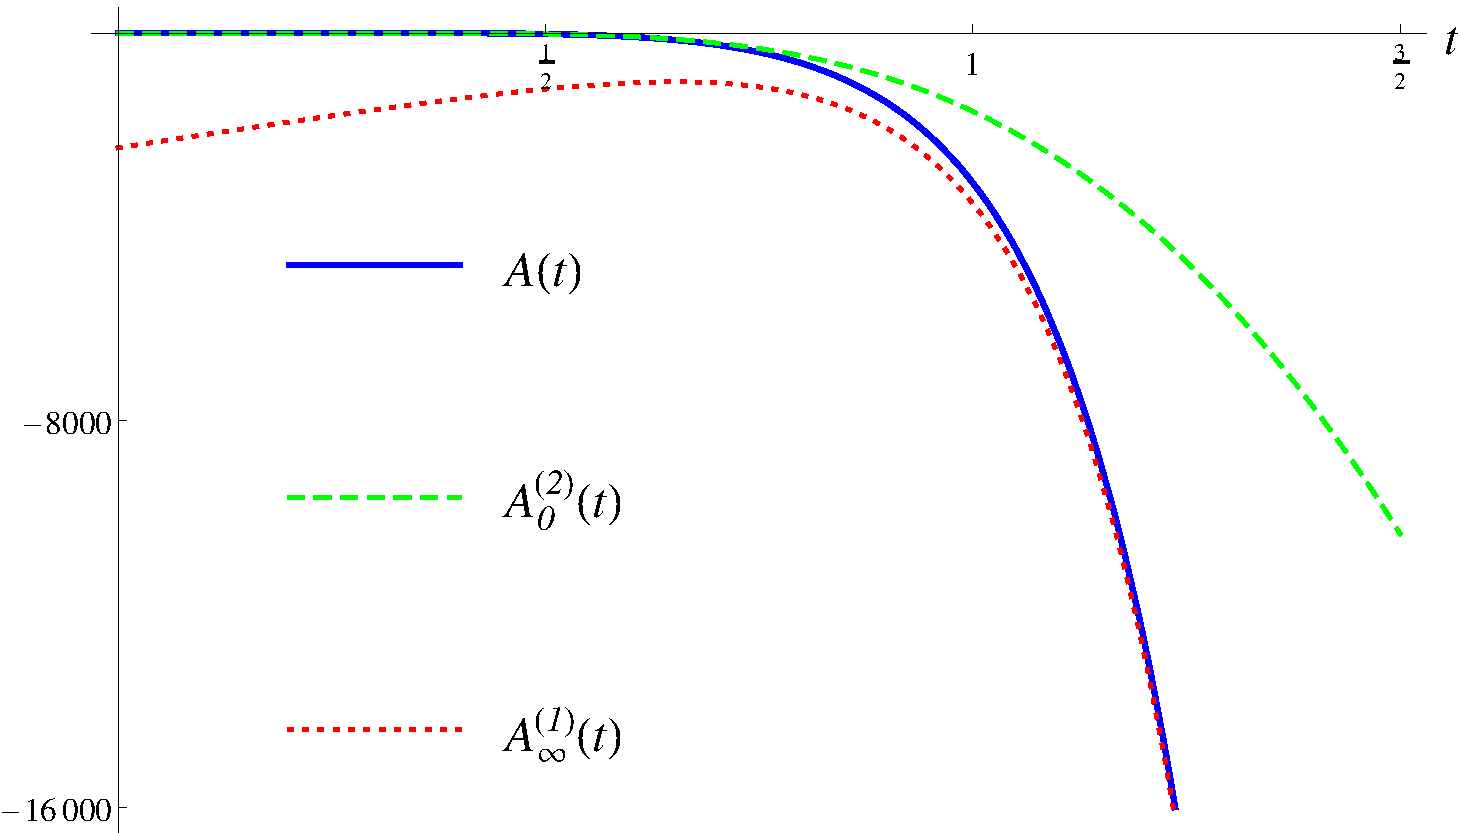
\includegraphics[width=300 pt]{graphics/e8plot_A.pdf}
\end{figure}

\noindent We observe that we can compute the values of $A(t)$ for $t\in(0,\infty)$ with any given precision. Indeed, from identities \eqref{eqn: phi0 transform} and \eqref{eqn: psi S define} we obtain the following two presentations for $A(t)$
\begin{align}
  A(t)=&-t^2\phi_0(i/t)+\frac{36}{\pi^2}\,t^2\,\psi_S(i/t)\notag\\
  A(t)=&-t^2\phi_0(it)+\frac{12}{\pi}\,t\,\phi_{-2}(it)-\frac{36}{\pi^2}\,\phi_{-4}(it)-\frac{36}{\pi^2}\,\psi_I(i/t).\notag
\end{align}
For an integer $n\geq0$ let $A_0^{(n)}$ and  $A_{\infty}^{(n)}$ be the functions such that
\begin{align}
  A(t)=&A_0^{(n)}(t)+O(t^2\,e^{-\pi n /t})\quad\mbox{as}\;t\to0\label{eqn: A asymptotic expansion 0}\\
  A(t)=&A_\infty^{(n)}(t)+O(t^2\,e^{-\pi n t})\quad\mbox{as}\;t\to\infty.\label{eqn: A asymptotic expansion infty}
\end{align}
For each $n\geq 0$ we can compute these functions from the Fourier expansions \eqref{eqn: phi fourier0}--\eqref{eqn: phi fourier4}, \eqref{eqn: psi fourier I}, and \eqref{eqn: psi fourier S}.
  For example, from \eqref{eqn: phi fourier4}--\eqref{eqn: phi fourier0} and \eqref{eqn: psi fourier I} we compute
%$$A_\infty^{(0)}(t)=-\frac{72}{\pi^2}\,e^{2\pi t}$$ and
\begin{align}A_\infty^{(6)}(t)=&\scriptstyle-\tfrac{72}{\pi ^2}\, e^{2 \pi  t}-\tfrac{23328}{\pi ^2}+\tfrac{184320}{\pi ^2}\, e^{-\pi  t}-\tfrac{5194368}{\pi ^2}\, e^{-2 \pi  t}+\tfrac{22560768}{\pi ^2}\, e^{-3 \pi  t}-\tfrac{250583040}{\pi
    ^2}\, e^{-4 \pi  t}+\tfrac{869916672 }{\pi ^2}\,e^{-5 \pi  t}\notag\\&\scriptstyle+t(\tfrac{8640}{\pi }+\tfrac{2436480}{\pi }\, e^{-2 \pi  t}+\tfrac{113011200 }{\pi }\,e^{-4 \pi  t})-t^2(518400\,e^{-2 \pi  t}+31104000\,e^{-4 \pi  t}).\notag
\end{align}
From \eqref{eqn: phi fourier4}--\eqref{eqn: phi fourier0} and \eqref{eqn: psi fourier S} we compute
%$$A_0^{(2)}(t)=-\frac{368640}{\pi^2}\,t^2\,e^{-\pi /t}$$and
$$A_0^{(6)}(t)=t^2(-\tfrac{368640}{\pi ^2}\, e^{-\pi/t}-518400\, e^{-2\pi/t}-\tfrac{45121536}{\pi ^2}\, e^{-3\pi/t}-31104000\,e^{-4\pi/t}-\tfrac{1739833344}{\pi ^2}\, e^{-5\pi/t}).$$
Moreover, from the convergent asymptotic expansion for the Fourier coefficients of a weakly holomorphic modular form \cite[Proposition 1.12]{Bruinier} we find that the $n$-th Fourier coefficient $c_{\psi_I}(n)$ of $\psi_I$ satisfies
\begin{equation}\label{eqn: Fourier estimate 1}|c_{\psi_I}(n)|\leq e^{4\pi\sqrt{n}}\qquad n\in\tfrac 12 \Z_{>0}.\end{equation} Similar inequalities hold for the Fourier coefficients of $\psi_S$, $\phi_0$, $\phi_{-2}$, and $\phi_{-4}$:
\begin{align}\label{eqn: Fourier estimate 2}
&|c_{\psi_S}(n)|\leq 2e^{4\pi\sqrt{n}}\qquad n\in\tfrac 12 \Z_{>0} \\
&|c_{\phi_0}(n)|\leq 2e^{4\pi\sqrt{n}}\qquad n\in \Z_{>0} \\
&|c_{\phi_{-2}}(n)|\leq e^{4\pi\sqrt{n}}\qquad n\in  \Z_{>0} \\
&|c_{\phi_{-4}}(n)|\leq e^{4\pi\sqrt{n}}\qquad n\in \Z_{>0}. \label{eqn: Fourier estimate 5}
  \end{align}
Therefore, we can estimate the error terms in the asymptotic expansions \eqref{eqn: A asymptotic expansion 0} and \eqref{eqn: A asymptotic expansion infty} of $A(t)$
\begin{align}
\left|A(t)-A_0^{(m)}(t)\right|\leq& (t^2+\frac{36}{\pi^2})\,\sum_{n=m}^\infty 2e^{2\sqrt{2}\pi\sqrt{n}}\,e^{-\pi n/t}\notag\\
\left|A(t)-A_\infty^{(m)}(t)\right|\leq& (t^2+\frac{12}{\pi}\,t+\frac{36}{\pi^2})\,\sum_{n=m}^\infty 2e^{2\sqrt{2}\pi\sqrt{n}}\,e^{-\pi nt}.\notag
\end{align}
  For an integer $m\geq0$ we set
\begin{align}
R^{(m)}_0:=&(t^2+\frac{36}{\pi^2})\,\sum_{n=m}^\infty 2e^{2\sqrt{2}\pi\sqrt{n}}\,e^{-\pi n/t}\notag\\
R^{(m)}_\infty:=&(t^2+\frac{12}{\pi}\,t+\frac{36}{\pi^2})\,\sum_{n=m}^\infty 2e^{2\sqrt{2}\pi\sqrt{n}}\,e^{-\pi nt}.\notag
\end{align}
Using interval arithmetic we check that
\begin{align}
&\left|R_0^{(6)}(t)\right|\leq\left|A_0^{(6)}(t)\right|\quad\mbox{ for }\;t\in(0,1]\notag\\
&\left|R_\infty^{(6)}(t)\right|\leq\left|A_\infty^{(6)}(t)\right|\quad\mbox{ for }\;t\in[1,\infty)\notag\\
&A_0^{(6)}(t)<0\quad\mbox{ for }\;t\in(0,1]\notag\\
&A_\infty^{(6)}(t)<0\quad\mbox{ for }\;t\in[1,\infty).\notag
\end{align}
Thus, we see that $A(t)<0$ for $t\in (0,\infty)$. Then identity \eqref{eqn: g A} implies \eqref{eqn: g1}.


Next, we prove \eqref{eqn: g2}. By Propositions~\ref{prop: a another integral} and~\ref{prop: b another integral} we know that for $r>0$
\begin{equation}\label{eqn: g B} \widehat{g}(r)=\frac{\pi}{2160}\,\sin(\pi r^2/2)^2\,\int\limits_0^\infty B(t)\,e^{-\pi r^2 t}\,dt\end{equation}
where $$B(t)=-t^2\phi_0(i/t)+\frac{36}{\pi^2}\,\psi_I(it).$$
This function can be also written as
\begin{align}
  B(t)=&-t^2\phi_0(i/t)-\frac{36}{\pi^2}\,t^2\,\psi_S(i/t)\notag\\
  B(t)=&-t^2\phi_0(it)+\frac{12}{\pi}\,t\,\phi_{-2}(it)-\frac{36}{\pi^2}\,\phi_{-4}(it)+\frac{36}{\pi^2}\,\psi_I(i/t).\notag
\end{align}
Our aim is to prove that $B(t)>0$ for $t\in(0,\infty)$. A plot of $B(t)$ is given in Figure~\ref{fig:B}.
\begin{figure}[h!]
\caption{Plot of the functions $B(t)$, $B^{(2)}_0(t)=\frac{368640}{\pi^2}\,t^2\,e^{-\pi /t}$, and $B^{(1)}_\infty(t)=\frac{8640}{\pi}t-\frac{23328}{\pi^2}$.\label{fig:B}}
  \centering
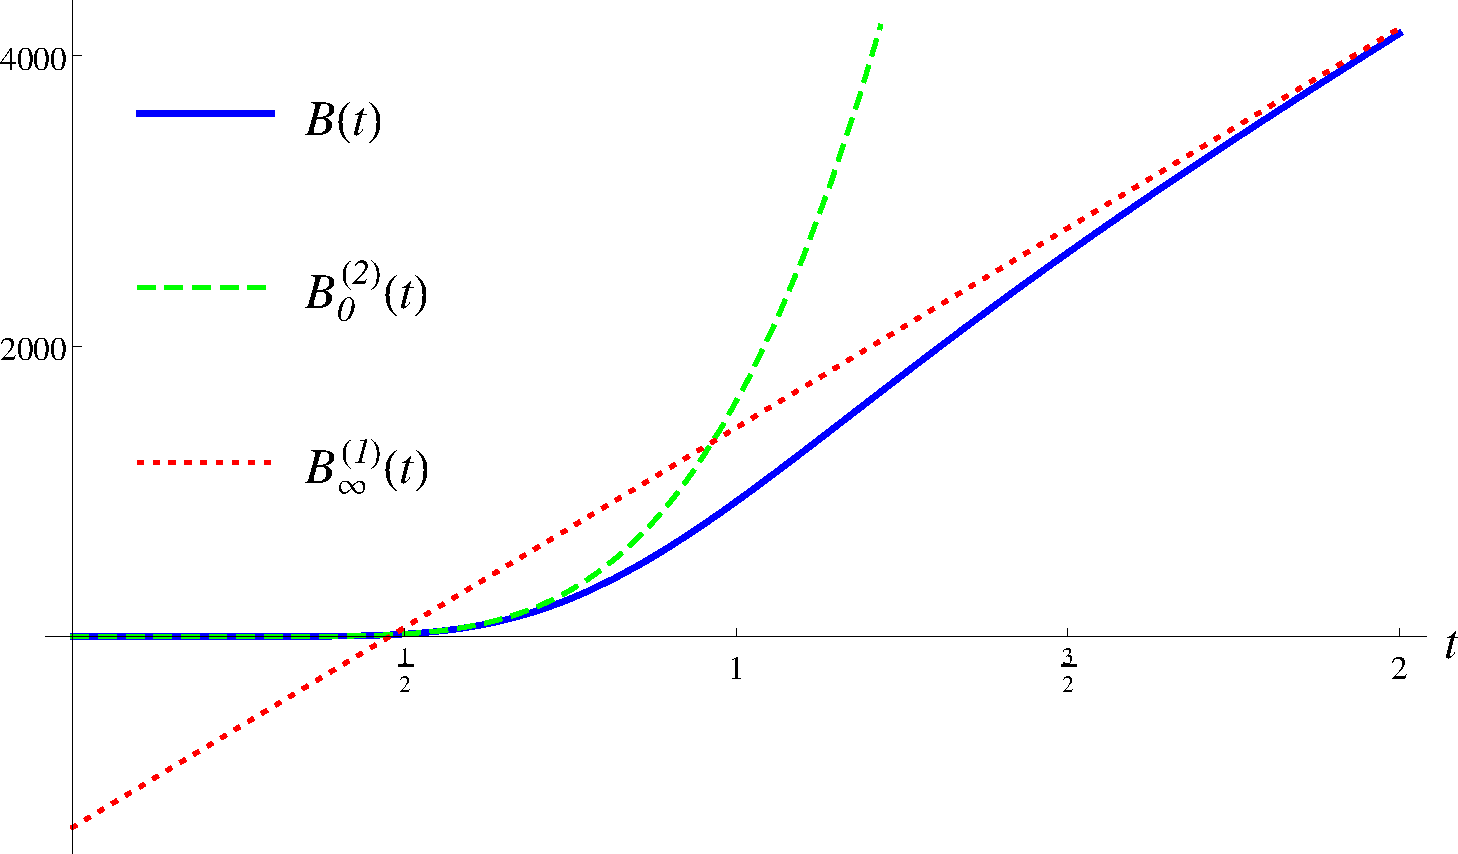
\includegraphics[width=300 pt]{graphics/e8plot_B.pdf}
\end{figure}

\noindent For $n\geq 0$ let $B_0^{(n)}$ and  $B_{\infty}^{(n)}$ be the functions  such that
\begin{align}
  B(t)=&B_0^{(n)}(t)+O(t^2\,e^{-\pi n /t})\quad\mbox{as}\;t\to0\notag\\
  B(t)=&B_\infty^{(n)}(t)+O(t^2\,e^{-\pi n t})\quad\mbox{as}\;t\to\infty.\notag
\end{align}
We find
\begin{align}B_\infty^{(6)}(t)=&-\tfrac{12960}{\pi ^2}-\tfrac{184320}{\pi ^2}\,\scriptstyle e^{-\pi  t}\displaystyle-\tfrac{116640}{\pi ^2} \,\scriptstyle e^{-2\pi  t}\displaystyle-\tfrac{22560768}{\pi ^2}\,\scriptstyle e^{-3\pi  t}\displaystyle+\tfrac{56540160}{\pi ^2}\,\scriptstyle e^{-4\pi  t}\displaystyle-\tfrac{869916672 }{\pi ^2} \,\scriptstyle e^{-5\pi  t}\displaystyle\notag\\
&+t(\tfrac{8640 }{\pi }+\tfrac{2436480}{\pi }\,\scriptstyle e^{-2\pi  t}\displaystyle+\tfrac{113011200 }{\pi }\,\scriptstyle e^{-4\pi  t}\textstyle)-t^2(\scriptstyle518400\,\scriptstyle e^{-2\pi  t}\displaystyle+\scriptstyle31104000\,\scriptstyle e^{-4\pi  t}\displaystyle)\notag
\end{align}
and
$$B_0^{(6)}(t)= t^2(\tfrac{368640}{\pi ^2}\, e^{-\pi/t}-518400\, e^{-2 \pi /t}+\tfrac{45121536 }{\pi ^2}\,e^{-3 \pi/t}-31104000\, e^{-4 \pi/t}+\tfrac{1739833344 }{\pi ^2}\,e^{-5 \pi/t}) .$$
The estimates \eqref{eqn: Fourier estimate 1}--\eqref{eqn: Fourier estimate 5} imply that $$\left|B(t)-B_0^{(6)}(t)\right|\leq R_0^{(6)}(t)\quad\mbox{for}\;t\in(0,1]$$
and
$$\left|B(t)-B_\infty^{(6)}(t)\right|\leq R_\infty^{(6)}(t)\quad\mbox{for}\;t\in[1,\infty).$$
Using interval arithmetic we verify that
\begin{align}
&\left|R_0^{(6)}(t)\right|\leq\left|B_0^{(6)}(t)\right|\quad\mbox{ for }\;t\in(0,1]\notag \\
&\left|R_\infty^{(6)}(t)\right|\leq\left|B_\infty^{(6)}(t)\right|\quad\mbox{ for }\;t\in[1,\infty)\notag \\
&B_0^{(6)}(t)>0\quad\mbox{ for }\;t\in(0,1]\notag \\
&B_\infty^{(6)}(t)>0\quad\mbox{ for }\;t\in[1,\infty). \notag
\end{align}
Now identity \eqref{eqn: g B} implies \eqref{eqn: g2}.

Finally, the property \eqref{eqn: g3} readily follows from Proposition~\ref{prop: a values} and Proposition~\ref{prop: b values}.
This finishes the proof of Theorems~\ref{thm: g1} and~\ref{thm: g}.
  \end{proof}




\begin{thebibliography}{10}
\bibitem{Abramowitz} {\sc M. Abramowitz, I. Stegun}, \emph{ Handbook of Mathematical Functions with Formulas, Graphs, and Mathematical Tables}, Applied Mathematics Series 55 (10 ed.), New York, USA: United States Department of Commerce, National Bureau of Standards; Dover Publications, 1964.

%\bibitem{BRV} {\sc A. Bondarenko, D. Radchenko, M. Viazovska}, \emph{On optimal asymptotic bounds for spherical designs}, Annals of Math. 178 (2)(2013), pp. 443--452.

\bibitem{Bruinier} {\sc J. Bruinier}, \emph{Borcherds products on O(2,l) and Chern classes of Heegner divisors}, Springer Lecture Notes in Mathematics 1780 (2002)

\bibitem{ElkiesCohn}  {\sc H. Cohn, N. Elkies}, \emph{New upper bounds on sphere packings I}, Annals of Math. 157 (2003) pp. 689--714.

%\bibitem{Cohn} {\sc H. Cohn}, \emph{New upper bounds on sphere packings. II.} Geom. Topol. 6 (2002), pp. 329--353.

%\bibitem{CohnKumar} {\sc H. Cohn, A. Kumar}, \emph{Universally optimal distribution of points on spheres}, J. Amer. Math. Soc. 20 (1) (2007), pp. 99--148.

%\bibitem{ConwaySloan}  {\sc J. H. Conway and N. J. A. Sloane}, \emph{What Are All the Best Sphere Packings in Low Dimensions? ,} Discrete Comput. Geom. (Laszlo Fejes Toth Festschrift), 13 (1995), pp. 383--403.


%\bibitem{DukeImamogluToth} {\sc W. Duke, O. Imamoglu and A. Toth}, {\em Cycle integrals of the j-function and mock modular forms}, Ann. of Math. (2) 173 (2011), no. 2, 947-981.

%\bibitem{Deligne1} {\sc P. Deligne}, \emph{Travaux de Shimura.} S\'eminaire Bourbaki, 23\'eme ann\'ee (1970/71), Exp. No. 389, pp. 123-165. Lecture Notes in Math., Vol. 244, Springer, Berlin, 1971.

%\bibitem{Deligne2} {\sc P. Deligne}, \emph{Vari\'et\'es de Shimura: interpr\'etation modulaire, et techniques de construction de mod\'eles canoniques}, in Automorphic forms, representations and L-functions, Proc. Sympos. Pure Math., XXXIII (Corvallis, OR, 1977), Part 2, pp. 247-289, Amer. Math. Soc., Providence, R.I., 1979.



%\bibitem{CohnZ} {\sc H. Cohn, Y. Zhao}, \emph{Sphere packing bounds via spherical codes}, arXiv:1212.5966 [math.MG]

%\bibitem{Delsarte72} {\sc P. Delsarte},\emph{Bounds for unrestricted codes, by linear programming}, Philips Res. Rep. 27 (1972), pp. 272--289.


%\bibitem{Delsarte77} {\sc P. Delsarte, J. M. Goethals, and J. J. Seidel}, \emph{Spherical codes and designs}, Geom. Dedicata, 6 (1977), pp. 363--388.

\bibitem{first course} {\sc F. Diamond, J. Shurman}, \emph{A First Course in Modular Forms}, Springer New York, 2005.

%\bibitem{Toth} {\sc L. Fejes Toth}, {\em {\"U}ber die dichteste Kugellagerung}, Math. Z. 48 (1943), pp. 676--684.

%\bibitem{Hales} {\sc T. Hales}, {\em A proof of the Kepler conjecture}, Annals of Math. 162 (3) (2005), pp. 1065--1185.

\bibitem{Hejhal} {\sc D. Hejhal}, {\em The Selberg trace formula for $\mathrm{PSL}(2, \R)$},  Springer Lecture Notes in Mathematics 1001 (1983)

%\bibitem{KabLev} {\sc G. A. Kabatiansky and V. I. Levenshtein}, {\em Bounds for packings on a sphere and in space},Problems of Information Transmission 14 (1978), pp. 1--17.

\bibitem{Mumford} {\sc D. Mumford}, {\em Tata Lectures on Theta I}, Birkh\"auser, 1983.

%\bibitem{Ma} {\sc Manin, Yu. I.}, {\em Real multiplication and noncommutative geometry (ein Alterstraum)}. The legacy of Niels Henrik Abel, 685-727, Springer, Berlin, 2004.

%\bibitem{MaOdSl} {\sc C. L. Mallows, A. M. Odlyzko, and N. J. A. Sloane}, {\em Upper bounds for modular forms, lattices, and codes}, J. Algebra, 36 (1975), 68--76

\bibitem{Petersson32} {\sc H. Petersson}, {\em Ueber die Entwicklungskoeffizienten der automorphen Formen}, Acta Mathematica, Bd. 58 (1932),  pp. 169--215.

%\bibitem{PfenderZiegler} {\sc F. Pfender, G. M. Ziegler,} {\em Kissing numbers, sphere packings, and some unexpected proofs}, Notice of the AMS  51 (8) (2004) pp. 873--883

\bibitem{Rademacher38} {\sc H. Rademacher and H. S. Zuckerman}, {\em On the Fourier coefficients of certain modular forms of
positive dimension}, Annals of Math. (2) 39 (1938),  pp. 433--462.

%\bibitem{Thue} {\sc A. Thue}, {\em {\"U}ber die dichteste Zusammenstellung von kongruenten Kreisen in einer Ebene}, Norske Vid. Selsk. Skr. No.1 (1910), pp. 1--9.

%\bibitem{Venk}   {\sc  A. Venkatesh}, {\em A Note on Sphere Packings in High Dimension}, International Mathematics Research Notices  7 (2013),  1628--1642

%\bibitem{Yudin} {\sc V. A. Yudin}, {\em Lower bounds for spherical designs}, Izv. Ross. Akad. Nauk. Ser. Mat. 61 (1997), pp. 211-233. English transl., Izv. Math. 6 (1997), pp. 673--683.

\bibitem{1-2-3} {\sc D. Zagier}, {\em Elliptic Modular Forms and Their Applications}, In:  The 1-2-3 of Modular Forms, (K. Ranestad, ed.) Norway, Springer Universitext, 2008.
\end{thebibliography}

\newpage

{\footnotesize
\noindent
Ecole Polytechnique Federale de Lausanne\\
1015 Lausanne\\
Switzerland\\
{\it Email address: maryna.viazovska@epfl.ch}}

\end{document}


\plastexfalse

\title{Sphere Packing in Lean}
\author{Maryna Viazovska, Sidharth Hariharan}

\begin{document}
\maketitle
% In this file you should put the actual content of the blueprint.
% It will be used both by the web and the print version.
% It should *not* include the \begin{document}
%
% If you want to split the blueprint content into several files then
% the current file can be a simple sequence of \input. Otherwise It
% can start with a \section or \chapter for instance.

\begin{abstract}
  In this paper we prove that no packing of unit balls in Euclidean space $\R^8$ has density greater than that of the $E_8$-lattice packing.
  \ifplastex
  % web
  The PDF version of this blueprint is available \href{https://thefundamentaltheor3m.github.io/Sphere-Packing-Lean/blueprint.pdf}{here}.
  \else
  % print
  The web version of this blueprint is available \href{https://thefundamentaltheor3m.github.io/Sphere-Packing-Lean/blueprint/index.html}{here}.
  \fi
  \end{abstract}


\section{Basic definitions for sphere packings}
\subsection{Sphere packings}
The sphere packing constant measures which portion of $d$-dimensional Euclidean
space can be covered by non-overlapping unit balls. More precisely, let $\R^d$ be the Euclidean vector space equipped with distance $\|\cdot\|$ and Lebesgue measure $\mathrm{Vol}(\cdot)$. For $x\in\R^d$ and $r\in\R_{>0}$ we denote by $B_d(x,r)$ the ball in $\R^d$ with center $x$ and radius $r$.

\begin{definition}\label{SpherePacking.isPacking}\lean{SpherePacking.isPacking}\leanok
  Let $X\subset \R^d$ be a discrete set of points such that $\|x-y\|\geq2$ for any distinct $x,y\in X$. Then the union
$$\mathcal{P}=\bigcup_{x\in X} B_d(x,1)$$ is a \emph{sphere packing}.
\end{definition}

\begin{definition}\label{SpherePacking.isLatticePacking}\uses{EuclideanLattice.is_lattice}\lean{SpherePacking.isLatticePacking}\leanok
  If $X$ is a lattice in $\R^d$ then we say that $\mathcal{P}$ is a \emph{lattice sphere packing}.
\end{definition}

\begin{definition}\label{SpherePacking.FiniteDensity}\lean{SpherePacking.FiniteDensity}\leanok
  The \emph{finite density} of a packing $\mathcal{P}$ is defined as
$$\Delta_{\mathcal{P}}(r):=\frac{\mathrm{Vol}(\mathcal{P}\cap B_d(0,r))}{\mathrm{Vol}(B_d(0,r))},\quad r>0.$$
\end{definition}

\begin{definition}\label{SpherePacking.Density}\uses{SpherePacking.FiniteDensity}\lean{SpherePacking.Density}\leanok
  We define the \emph{density} of a packing $\mathcal{P}$ as the limit superior
$$\Delta_{\mathcal{P}}:=\limsup\limits_{r\to\infty}\Delta_{\mathcal{P}}(r). $$
\end{definition}

\begin{definition}\label{SpherePacking.Constant}\uses{SpherePacking.isPacking, SpherePacking.Density}\lean{SpherePacking.Constant}\leanok
The number be want to know is the supremum over all possible packing densities
$$\Delta_d:=\sup\limits_{\substack{\mathcal{P}\subset\R^d\\ \scriptscriptstyle\mathrm{sphere}\;\mathrm{packing}}}\Delta_{\mathcal{P}} $$
called the \emph{sphere packing constant}.
\end{definition}

The main result of this paper is the proof that $$\Delta_8=\frac{\pi^4}{384}\approx 0.25367.$$
This is the density of the $E_8$-lattice sphere packing.

\begin{definition}\label{EuclideanLattice.E8}\lean{EuclideanLattice.E8}
  Recall that the $E_8$-lattice $\Lambda_8\subset\R^8$ is given by
$$\Lambda_8=\{(x_i)\in\Z^8\cup(\Z+\textstyle\frac12\displaystyle )^8|\;\sum_{i=1}^8x_i\equiv 0\;(\mathrm{mod\;2})\}.$$
\end{definition}
\begin{lemma}\label{lemma: Characterisation of E8 lattice}
  $\Lambda_8$ is a positive-definite, even, unimodular lattice of rank 8. The minimal distance between two points in $\Lambda_8$ is $\sqrt{2}$.
\end{lemma}
\begin{definition}\label{SpherePacking.E8}\uses{EuclideanLattice.E8}\lean{SpherePacking.E8}\leanok
The $E_8$-lattice sphere packing is the packing of unit balls with centers at $\frac{1}{\sqrt{2}}\Lambda_8$.
\end{definition}
Our main result is
\begin{theorem}\label{SpherePacking.Main}\lean{SpherePacking.Main}
No packing of unit balls
in Euclidean space $\R^8$ has density greater than that of the $E_8$-lattice packing.
\end{theorem}

\subsection{Lattices and Periodic packings}
\begin{definition}\label{def: Periodicity}
  Let $S$ be a discrete subgroup of $\R^d$. A set $X\subset\R^d$ is said to $S$-periodic if for each $s\in S$ and $x\in X$ the vector $x+s$ belongs to $X$.
\end{definition}

\begin{definition}\label{EuclideanLattice.is_lattice}\lean{EuclideanLattice.is_lattice}\leanok
  % A lattice in the Euclidean space $\R^d$ is a discrete, co-compact, abelian subgroup.
  A subset of the Euclidean space $\R^d$ is called a lattice if it is the $\Z$-span of a basis of $\R^d$.
\end{definition}

\begin{lemma}\label{SpherePacking.Density of periodic packing} \notready
  Density of a periodic packing ...
\end{lemma}
\subsection{Facts from Fourier analysis}
hello
In this subsection we recall a few definitions from Fourier analysis.
\begin{definition}\label{def: Fourier Transform definition} % \lean{def: Fourier Transform definition}
The Fourier transform of an $L^1$-function $f:\R^d\to\C$ is defined as
$$\mathcal{F}(f)(y)=\widehat{f}(y):=\int\limits_{\R^d} f(x)\,e^{-2\pi i x\cdot y}\,dx,\quad y\in\R^d $$
where $x\cdot y=\frac12\|x\|^2+\frac12\|y\|^2-\frac12\|x-y\|^2$ is the standard scalar product in $\R^d$.
\end{definition}
\begin{definition}
A $C^\infty$~function $f:\R^d\to\C$ is called a \emph{Schwartz function} if it goes to zero as $\|x\|\to\infty$ faster then any inverse power of $\|x\|$, and the same holds for all partial derivatives of $f$. The set of all Schwartz functions is called a \emph{Schwartz space}.
\end{definition}
\begin{lemma}\label{lemma: Fourier transform is automorphism}
  The Fourier transform is an automorphism of the space of Schwartz functions.
\end{lemma}
\begin{lemma}\label{lemma: Gaussian Fourier}\uses{def: Fourier Transform definition}
\begin{equation}\mathcal{F}(e^{\pi i  \|x\|^2 z})(y)=z^{-4}\,e^{\pi i \|y\|^2 \,(\frac{-1}{z}) }.\end{equation}
\end{lemma}
\begin{theorem}\label{thm: Poisson summation formula}\uses{def: Fourier Transform definition}
  (Poisson summation formula)$$\sum_{\ell\in\Lambda}f(\ell)=\frac{1}{\mathrm{vol}(\R^d/\Lambda)}\sum_{m\in\Lambda^*}\widehat{f}(m).$$
\end{theorem}

\section{Cohn-Elkies linear programming bounds}

In 2003 Cohn and Elkies \cite{ElkiesCohn}  developed  linear programming bounds that apply directly to sphere packings. The goal of this section is to formalize the Cohn--Elkies linear programming bound.

The following theorem is the key result of \cite{ElkiesCohn}. (The original theorem is stated for a   class of functions more general then Schwartz functions)
\begin{theorem}\label{thm: Cohn-Elkies}\uses{def: Fourier Transform definition}\uses{thm: Poisson summation formula}
(Cohn, Elkies \cite{ElkiesCohn}) Suppose that  $f:\R^d\to\R$ is a Schwartz function, is not identically zero, and satisfies:
\begin{equation}\label{eqn: Cohn-Elkies condition 1}f(x)\leq 0\mbox{ for } \|x\|\geq 1\end{equation} and
\begin{equation}\label{eqn: Cohn-Elkies condition 2}\widehat{f}(x)\geq0\mbox{ for all } x\in\R^d.\end{equation}
  Then the  density of  $d$-dimensional
  sphere packings is bounded above by $$\frac{f(0)}{\widehat{f}(0)}\cdot \frac{\pi^{\frac{d}{2}}}{2^d\,\Gamma(\textstyle \frac{d}{2}+1)}.$$
\end{theorem}
\begin{proof}
To be included.
\end{proof}


  The main step in our proof of Theorem \ref{SpherePacking.Main} is the explicit  construction of an optimal function. It will be convenient for us to scale this function by $\sqrt{2}$.
\begin{theorem}\label{thm: g}
There exists a radial Schwartz function $g:\R^8\to\R$ which satisfies:
\begin{align}
g(x)&\leq 0\mbox{ for } \|x\|\geq \sqrt{2} \label{eqn: g1}\\
\widehat{g}(x)&\geq0\mbox{ for all } x\in\R^8\label{eqn: g2}\\
g(0)&=\widehat{g}(0)=1.\label{eqn: g3}
\end{align}
\end{theorem}
Theorem \ref{thm: Cohn-Elkies} applied to the optimal function $f(x)=g(x/\sqrt{2})$ immediately implies Theorem \ref{SpherePacking.Main}.


\section{Modular forms}
Let $\h$ be the upper half-plane $\{z\in\C\mid\Im(z)>0\}$. The modular group $\Gamma_1:=\mathrm{PSL}_2(\Z)$ acts on $\h$ by linear fractional transformations
$$\left(\begin{smallmatrix}a&b\\c&d\end{smallmatrix}\right)z:=\frac{az+b}{cz+d}.$$

Let $N$ be a positive integer. The \emph{level $N$ principal congruence subgroup} of $\Gamma_1$ is
$$\Gamma(N):=\left\{\left.\left(\begin{smallmatrix}a&b\\c&d\end{smallmatrix}\right)\in\Gamma_1\right|\left(\begin{smallmatrix}a&b\\c&d\end{smallmatrix}\right)\equiv\left(\begin{smallmatrix}1&0\\0&1\end{smallmatrix}\right)\;\mathrm{mod}\;N\right\}.$$
A subgroup $\Gamma\subset\Gamma_1$ is called a \emph{congruence subgroup} if $\Gamma(N)\subset\Gamma$ for some $N\in\N$. An important example of a congruence subgroup is
$$\Gamma_0(N):=\left\{\left.\left(\begin{smallmatrix}a&b\\c&d\end{smallmatrix}\right)\in\Gamma_1\right|\;c\equiv0\;\mathrm{mod}\;N\right\}.$$

Let $z\in\h$, $k\in\Z$, and $\left(\begin{smallmatrix}a&b\\c&d\end{smallmatrix}\right)\in\mathrm{SL}_2(\Z)$. The \emph{automorphy factor} of weight $k$ is defined as
$$j_k(z,\left(\begin{smallmatrix}a&b\\c&d\end{smallmatrix}\right)):=(cz+d)^{-k}.$$
The automorphy factor satisfies the \emph{chain rule}
$$j_k(z,\gamma_1\gamma_2)=j_k(z,\gamma_1)\,j_k(\gamma_2z,\gamma_1). $$
Let $F$ be a  function on $\h$ and $\gamma\in\mathrm{PSL}_2(\Z)$. Then the \emph{slash operator} acts on $F$ by
$$(F|_k\gamma)(z):=j_k(z,\gamma)\,F(\gamma z). $$
The chain rule implies
$$F|_k\gamma_1\gamma_2=(F|_k\gamma_1)|_k\gamma_2.$$

\begin{definition}\label{def: holomorphic modular form}% \lean{def: holomorphic modular form}
A \emph{(holomorphic) modular form} of integer weight $k$ and congruence subgroup $\Gamma$ is a holomorphic function $f:\h\to\C$ such that:
\begin{enumerate}
  \item $f|_k\gamma=f$ for all $\gamma\in\Gamma$
  \item for each $\alpha\in\Gamma_1\;f|_k\alpha$ has the Fourier expansion $f|_k\alpha (z)=\sum_{n=0}^\infty c_f(\alpha,\frac{n}{n_\alpha})\,e^{2\pi i \frac{n}{n_\alpha}z}$ for some $n_\alpha\in\N$ and Fourier coefficients $c_f(\alpha,m)\in\C$.
\end{enumerate}
\end{definition}

Let $M_k(\Gamma)$ be the space of modular forms of weight $k$ and congruence subgroup $\Gamma$. A key fact in the theory of modular forms is that the spaces $M_k(\Gamma)$ are finite dimensional.

Let us consider several examples of modular forms.
\begin{definition}\label{def: Ek definition}% \lean{def: Ek definition}
For an even integer $k\geq 4$ we define the \emph{weight $k$ Eisenstein series} as
\begin{equation}\label{eqn: Ek definition}E_k(z):=\frac{1}{2\zeta(k)}\sum_{(c,d)\in\Z^2\backslash(0,0)}(c\tau+d)^{-k}.\end{equation}
\end{definition}
Since the sum converges absolutely, it is easy to see that $E_k\in M_k(\Gamma_1)$.
\begin{lemma}\label{lemma: Ek Fourier}
% \lean{lemma: Ek Fourier}\uses{def: Ek definition}
The Eisenstein series possesses the Fourier expansion
\begin{equation}\label{eqn: Ek Fourier}E_k(z)=1+\frac{2}{\zeta(1-k)}\sum_{n=1}^\infty \sigma_{k-1}(n)\,e^{2\pi i z}, \end{equation}
where $\sigma_{k-1}(n)\,=\,\sum_{d|n} d^{k-1}$. In particular, we have
\begin{align}
  E_4(z)\,=\,& 1+240\sum_{n=1}^\infty \sigma_3(n)\,e^{2\pi i n z} \notag \\
  E_6(z)\,=\,& 1-504\sum_{n=1}^\infty \sigma_5(n)\,e^{2\pi i n z}. \notag
\end{align}
\end{lemma}
The infinite sum \eqref{eqn: Ek definition} does not converge absolutely for $k=2$. On the other hand, the expression \eqref{eqn: Ek Fourier} converges to a holomorphic function on the upper half-plane and therefore
\begin{definition} \label{def: E2 def} % \lean{def: E2 def}
We set
\begin{equation}E_2(z):= 1-24\sum_{n=1}^\infty \sigma_1(n)\,e^{2\pi i n z}.\notag\end{equation}
\end{definition}
\begin{lemma}
\label{lemma: E2 transform}

% \lean{lemma: Ek Fourier}

This function is not modular, however it satisfies
\begin{equation}\label{eqn: E2 transform}z^{-2}\,E_2\Big(\frac{-1}{z}\Big)=E_2(z) -\frac{6i}{\pi}\, \frac{1}{z}.\end{equation}
\end{lemma}
The proof of this identity can be found in \cite[Section~2.3]{1-2-3}.
The weight two Eisenstein series $E_2$ is an example of a \emph{quasimodular form} \cite[Section~5.1]{1-2-3}.

Another example of modular forms we would like to consider are \emph{theta functions} \cite[Section~3.1]{1-2-3}.
We define three different theta functions (so called ``Thetanullwerte'') as
\begin{align}
  \theta_{00}(z)\,=\, & \sum_{n\in\Z}e^{\pi i n^2 z} \notag \\
  \theta_{01}(z)\,=\, & \sum_{n\in\Z}(-1)^n\,e^{\pi i n^2 z} \notag \\
  \theta_{10}(z)\,=\, & \sum_{n\in\Z}e^{\pi i (n+\frac12)^2 z}. \notag
\end{align}
The group $\Gamma_1$ is generated by the elements $T=\left(\begin{smallmatrix}1&1\\0&1\end{smallmatrix}\right)$ and $S=\left(\begin{smallmatrix}0&1\\-1&0\end{smallmatrix}\right)$.
\begin{lemma}\label{lemma: theta transform S T}
% \lean{lemma: theta transform S T}

These elements  act on the theta functions in the following way
\begin{align}
z^{-2}\,\theta^4_{00}\Big(\frac{-1}{z}\Big)\,=\,&-\theta_{00}^4(z) \label{eqn: theta transform S}\\
z^{-2}\,\theta^4_{01}\Big(\frac{-1}{z}\Big)\,=\,&-\theta_{10}^4(z)\\
z^{-2}\,\theta^4_{10}\Big(\frac{-1}{z}\Big)\,=\,&-\theta_{01}^4(z)
\end{align}
and
\begin{align}
\theta^4_{00}(z+1)\,=\,&\theta_{01}^4(z)\\
\theta^4_{01}(z+1)\,=\,&\theta_{00}^4(z)\\
\theta^4_{10}(z+1)\,=\,&-\theta_{10}^4(z). \label{eqn: theta transform T}
\end{align}
\end{lemma}
Moreover, these three theta functions satisfy the \emph{Jacobi identity}
\begin{equation}
\theta_{01}^4+\theta_{10}^4=\theta_{00}^4.
\end{equation}
The theta functions $\theta^4_{00},\theta^4_{01}$, and $\theta^4_{10}$ belong to $M_2(\Gamma(2))$.


\begin{definition}\label{def: weakly-holomorphic modular form}
A \emph{weakly-holomorphic modular form} of integer weight $k$ and congruence subgroup $\Gamma$ is a holomorphic function $f:\h\to\C$ such that:
\begin{enumerate}
  \item $f|_k\gamma=f$ for all $\gamma\in\Gamma$
  \item for each $\alpha\in\Gamma_1\;f|_k\alpha$ has the Fourier expansion $f|_k\alpha (z)=\sum_{n=n_0}^\infty c_f(\alpha,\frac{n}{n_\alpha})\,e^{2\pi i \frac{n}{n_\alpha}z}$ for some $n_0\in\Z$ and $n_\alpha\in\N$.
\end{enumerate}
\end{definition}
For an $m$-periodic holomorphic function $f$ and $n\in\frac 1m \Z$ we will denote the $n$-th Fourier coefficient of $f$ by $c_f(n)$ so that
$$f(z)=\sum_{n\in\frac 1m \Z} c_f(n)\,e^{2\pi i n z}.$$
We denote the space of weakly-holomorphic modular forms of weight $k$ and group $\Gamma$ by $M_k^!(\Gamma)$. The spaces $M_k^!(\Gamma)$ are infinite dimensional.
Probably the most famous weakly-holomorphic modular form is the \emph{elliptic j-invariant}
$$j\,:=\,\frac{1728\, E_4^3}{E_4^3-E_6^2}. $$
This function belongs to $M_0^!(\Gamma_1)$ and has the Fourier expansion
$$j(z)\,=\,q^{-1} + 744 + 196884\, q + 21493760\, q^2 + 864299970\, q^3 +
  20245856256\, q^4 + O(q^5) $$
  where $q=e^{2\pi i z}$. Using a simple computer algebra system such as PARI GP or Mathematica one can compute first hundred terms of this Fourier expansion within few seconds. An important question is to find an  asymptotic formula for $c_j(n)$, the $n$-th Fourier coefficient  of $j$. Using the Hardy-Ramanujan circle method \cite{Rademacher38} or the non-holomorphic Poincare series \cite{Petersson32} one can show that
  \begin{lemma}\label{lemma: j Fourier asymptotic}
  % \lean{lemma: j Fourier asymptotic}
  \begin{equation}\label{eqn: j Fourier asymptotic}
  c_j(n)=\frac{2\pi}{n}\sum_{k=1}^\infty \frac{A_k(n)}{k}\,I_1\left(\frac{4\pi \sqrt{n}}{k}\right)\qquad n\in\Z_{>0}\end{equation}
  where
  $$A_k(n)= \sum_{\substack{h\;\mathrm{mod}\;k\\(h,k)=1}} e^{\frac{-2\pi i}{k}(nh+h')},\quad hh'\equiv -1(\mbox{mod}\;k),$$
  and $I_\alpha(x)$ denotes the modified Bessel function of the first kind defined as in \cite[Section~9.6]{Abramowitz}.
  \end{lemma}
  A similar convergent asymptotic expansion holds for the Fourier coefficients of any weakly holomorphic modular form \cite{Hejhal}, \cite[Propositions~1.10 and~1.12]{Bruinier}. Such a convergent expansion implies effective estimates for the Fourier coefficients.




\section{Fourier eigenfunctions with double zeroes at lattice points}\label{sec: fourier double zeroes}
In this section we construct two radial Schwartz functions $a,b:\R^8\to i\R$ such that
\begin{align}\mathcal{F}(a)&=a\label{eqn: a fourier}\\
  \mathcal{F}(b)&=-b\label{eqn: b fourier}
\end{align}
which double zeroes at all $\Lambda_8$-vectors of length greater than $\sqrt{2}$. Recall that each vector of $\Lambda_8$ has length $\sqrt{2n}$ for some $n\in\N_{\geq 0}$. We define $a$ and $b$ so that their values are purely imaginary because this simplifies some of our computations. We will show in Section \ref{sec: g} that an appropriate linear combination of functions $a$ and $b$ satisfies conditions \eqref{eqn: g1}--\eqref{eqn: g3}.

First, we will define function $a$. To this end we consider the following functions:
\begin{definition}\label{def: phi4 phi2 phi0}
\uses{def: Ek definition}
\begin{align}
  \phi_{-4}\,:= \,& -Dj\,E_6^{-1}\label{eqn: def phi4}\\
  \phi_{-2}\,:= \,&\phi_{-4}\,E_2+Dj\,E_4^{-1}\label{eqn: def phi2}\\
  \phi_{0}\,:= \,&\phi_{-4}\,E_2^2+2Dj\,E_4^{-1}\,E_2+j-1728.\label{eqn: def phi0}
\end{align}
\end{definition}
Here $Dj(z)=\frac{1}{2\pi i} \frac{d}{dz} j(z)$.
\begin{lemma}\label{lemma: phi fourier4 phi fourier2 phi fourier0}
  These functions have the Fourier expansions
\begin{align}
  \phi_{-4}(z)\,=\,&q^{-1} + 504 + 73764\, q + 2695040\, q^2 + 54755730\, q^3 + O(q^4)\label{eqn: phi fourier4}\\
  \phi_{-2}(z)\,=\,&720 + 203040\, q + 9417600\, q^2 + 223473600\, q^3 + 3566782080\, q^4+O(q^5)\label{eqn: phi fourier2}\\
  \phi_{0}(z)\,=\,&518400\, q + 31104000\, q^2 + 870912000\, q^3 + 15697152000\, q^4+O(q^5)\label{eqn: phi fourier0}
\end{align}
where $q=e^{2\pi i z}$.
\end{lemma}
The function $\phi_0(z)$ is not modular; however,
\begin{lemma}\label{lemma: phi0 transform}
  The identity \ref{lemma: E2 transform} implies the following transformation rule:
\begin{equation}\label{eqn: phi0 transform}
\phi_0\Big(\frac{-1}{z}\Big)=\phi_0(z)-\frac{12i}{\pi}\,\frac{1}{z}\,\phi_{-2}(z)-\frac{36}{\pi^2}\,\frac{1}{z^2}\,\phi_{-4}(z).
\end{equation}
\end{lemma}
\begin{definition}\label{def: a(r) definition}
For $x\in\R^8$ we define
\begin{align}\label{eqn: a(r) definition}
  a(x):=&\int\limits_{-1}^i\phi_0\Big(\frac{-1}{z+1}\Big)\,(z+1)^2\,e^{\pi i \|x\|^2 z}\,dz
  +\int\limits_{1}^i\phi_0\Big(\frac{-1}{z-1}\Big)\,(z-1)^2\,e^{\pi i \|x\|^2 z}\,dz\\
  -&2\int\limits_{0}^i\phi_0\Big(\frac{-1}{z}\Big)\,z^2\,e^{\pi i \|x\|^2 z}\,dz
  +2\int\limits_{i}^{i\infty}\phi_0(z)\,e^{\pi i \|x\|^2 z}\,dz.\nonumber
\end{align}
\end{definition}
We observe that the contour integrals in \eqref{eqn: a(r) definition} converge absolutely and uniformly for  $x\in\R^8$. Indeed,
$\phi_0(z)=O(e^{-2\pi i z})$ as $\Im(z)\to \infty$. Therefore, $a(x)$ is well defined. Now we prove that $a$ satisfies condition \eqref{eqn: a fourier}.
\begin{proposition}\label{prop: a(r) Fourier}\uses{lemma: Ek Fourier}\uses{def: E2 def}\uses{lemma: j Fourier asymptotic}\uses{def: a(r) definition}\uses{lemma: Gaussian Fourier}

The function $a$ defined by \eqref{eqn: a(r) definition} belongs to the Schwartz space and satisfies $$\widehat{a}(x)=a(x). $$
\end{proposition}
\begin{proof}
First, we prove that $a$ is a Schwartz function. From Lemma \ref{lemma: Ek Fourier}, Definition \ref{def: E2 def}, and \ref{lemma: j Fourier asymptotic} we deduce that the Fourier coefficients of $\phi_0$ satisfy
$$|c_{\phi_0}(n)|\leq2\,e^{4\pi\sqrt{n}}\quad n\in\Z_{>0}.$$ Thus, there exists a positive constant $C$ such that
$$|\phi_0(z)|\leq C\,e^{-2\pi \Im{z}}\qquad \mbox{for } \; \Im{z}>\frac 12.$$
We estimate the first summand in the right-hand side of \eqref{eqn: a(r) definition}.  For $r\in\R_{\geq 0}$ we have
\begin{align}&\Bigg|\int\limits_{-1}^{i}\phi_0\Big(\frac{-1}{z+1}\Big)\,(z+1)^2\,e^{\pi i r^2 z}\,dz\Bigg|=\Bigg|\int\limits_{i\infty}^{-1/(i+1)}\phi_0(z)\,z^{-4}\,e^{\pi i r^2 (-1/z-1)}\,dz\Bigg|\leq \notag\\
  &C_1\int\limits_{1/2}^{\infty}e^{-2\pi t}\,e^{-\pi  r^2/t}\,dt\leq C_1\int\limits_{0}^{\infty}e^{-2\pi t}\,e^{-\pi  r^2/t}\,dt=C_2\,r\,K_1(2\sqrt{2}\,\pi\,r)\notag
\end{align}
where $C_1$ and $C_2$ are some positive constants and $K_\alpha(x)$ is the modified Bessel function of the second kind defined as in \cite[Section~9.6]{Abramowitz}. This estimate also holds for the second and third summand in \eqref{eqn: a(r) definition}.
For the last summand we have
$$ \Bigg|\int\limits_{i}^{i\infty}\phi_0(z)\,e^{\pi i r^2 z}\,dz\Bigg|\leq C\,\int\limits_{1}^{\infty} e^{-2\pi t}\,e^{-\pi r^2 t}\,dt=C_3\frac{e^{\pi(r^2+2)}}{r^2+2}.$$
Therefore, we arrive at
$$|a(r)|\leq 4C_2\,r\,K_1(2\sqrt{2}\pi r)+2C_3\frac{e^{-\pi(r^2+2)}}{r^2+2}.$$
It is easy to see that the left hand side of this inequality decays faster then any inverse power of $r$. Analogous estimates can be obtained for all derivatives $\frac{d^k}{dr^k}a(r)$.

Now we show that $a$ is an eigenfunction of the Fourier transform. We recall that the Fourier transform of a Gaussian function is
\begin{equation}\label{eqn: Gaussian Fourier}\mathcal{F}(e^{\pi i  \|x\|^2 z})(y)=z^{-4}\,e^{\pi i \|y\|^2 \,(\frac{-1}{z}) }.\end{equation}
Next, we exchange the contour integration with respect to $z$ variable and Fourier transform  with respect to $x$ variable in \eqref{eqn: a(r) definition}. This can be done, since the corresponding double integral converges absolutely. In this way we obtain
\begin{align}
  \widehat{a}(y)=&\int\limits_{-1}^i\phi_0\Big(\frac{-1}{z+1}\Big)\,(z+1)^2\,z^{-4}\,e^{\pi i \|y\|^2 \,(\frac{-1}{z})}\,dz
  +\int\limits_{1}^i\phi_0\Big(\frac{-1}{z-1}\Big)\,(z-1)^2\,z^{-4}\,e^{\pi i \|y\|^2 \,(\frac{-1}{z})}\,dz\notag \\
  -&2\int\limits_{0}^i\phi_0\Big(\frac{-1}{z}\Big)\,z^2\,z^{-4}\,e^{\pi i \|y\|^2 \,(\frac{-1}{z})}\,dz +2\int\limits_{i}^{i\infty}\phi_0(z)\,z^{-4}\,e^{\pi i \|y\|^2 \,(\frac{-1}{z})}\,dz.\notag
\end{align}
Now we make a change of variables $w=\frac{-1}{z}$. We obtain
\begin{align}
  \widehat{a}(y)=&\int\limits_{1}^i\phi_0\Big(1-\frac{1}{w-1}\Big)\,(\frac{-1}{w}+1)^2\,w^{2}\,e^{\pi i \|y\|^2 \,w}\,dw\notag\\
  +&\int\limits_{-1}^i\phi_0\Big(1-\frac{1}{w+1}\Big)\,(\frac{-1}{w}-1)^2\,w^2\,e^{\pi i \|y\|^2 \,w}\,dw\\
  -&2\int\limits_{i \infty}^i\phi_0(w)\,e^{\pi i \|y\|^2 \,w}\,dw +2\int\limits_{i}^{0}\phi_0\Big(\frac{-1}{w}\Big)\,w^{2}\,e^{\pi i \|y\|^2 \,w}\,dw.\notag
\end{align}
Since $\phi_0$ is $1$-periodic we have
\begin{align}
  \widehat{a}(y)\,=\,&\int\limits_{1}^i\phi_0\Big(\frac{-1}{z-1}\Big)\,(z-1)^2\,e^{\pi i \|y\|^2 \,z}\,dz
  +\int\limits_{-1}^i\phi_0\Big(\frac{-1}{z+1}\Big)\,(z+1)^2\,e^{\pi i \|y\|^2 \,z}\,dz\notag \\
  +&2\int\limits_{i}^{i\infty}\phi_0(z)\,e^{\pi i \|y\|^2 \,z}\,dz
  -2\int\limits_{0}^{i}\phi_0\Big(\frac{-1}{z}\Big)\,z^{2}\,e^{\pi i \|y\|^2 \,z}\,dz\notag \\
  \,=\,&a(y).
\end{align}
This finishes the proof of the proposition.
\end{proof}

Next, we check that $a$ has double zeroes at all $\Lambda_8$-lattice points of length greater then $\sqrt{2}$.
%Note that by definition function $a$ is radial and therefore in naturally defines a function on $\R_{\geq0}$. For abuse of notation we denote this function also by $a$.

\begin{proposition}\label{prop: a(r) double zeroes}\uses{lemma:  phi0 transform}
For $r>\sqrt{2}$ we can express $a(r)$ in the following form
\begin{equation}\label{eqn: a double zeroes}
  a(r)=-4\sin(\pi r^2/2)^2\,\int\limits_{0}^{i\infty}\phi_0\Big(\frac{-1}{z}\Big)\,z^2\,e^{\pi i r^2 \,z}\,dz.
\end{equation}
\end{proposition}
\begin{proof}
We denote the right hand side of \eqref{eqn: a double zeroes} by $d(r)$.  It is easy to see that $d(r)$ is well-defined. Indeed, from the transformation formula \eqref{eqn: phi0 transform} and the expansions \eqref{eqn: phi fourier0}--\eqref{eqn: phi fourier4} we obtain
\begin{align}
\phi_0\Big(\frac{-1}{it}\Big)=&O(e^{-2\pi/t})\quad\mbox{as}\;t\to 0\notag\\
\phi_0\Big(\frac{-1}{it}\Big)=&O(t^{-2}\,e^{2\pi t})\quad\mbox{as}\;t\to \infty\notag
\end{align}
Hence, the integral \eqref{eqn: a double zeroes} converges absolutely for $r>\sqrt{2}$.
  We can write %\texttt{check signs}
\begin{align}
  d(r)=&\int\limits_{-1}^{i\infty-1}\phi_0\Big(\frac{-1}{z+1}\Big)\,(z+1)^2\,e^{\pi i r^2 \,z}\,dz-
  2\int\limits_{0}^{i\infty}\phi_0\Big(\frac{-1}{z}\Big)\,z^2\,e^{\pi i r^2 \,z}\,dz\notag\\
  +&\int\limits_{1}^{i\infty+1}\phi_0\Big(\frac{-1}{z-1}\Big)\,(z-1)^2\,e^{\pi i r^2 \,z}\,dz.\notag
\end{align}
From \eqref{eqn: phi0 transform} we deduce that if $r>\sqrt{2}$ then
$\phi_0\Big(\frac{-1}{z}\Big)\,z^2\,e^{\pi i r^2 \,z}\to 0$ as $\Im(z)\to\infty$. Therefore, we can deform the paths of integration
and rewrite
\begin{align}
  d(r)=&\int\limits_{-1}^{i}\phi_0\Big(\frac{-1}{z+1}\Big)\,(z+1)^2\,e^{\pi i r^2 \,z}\,dz
  +\int\limits_{i}^{i\infty}\phi_0\Big(\frac{-1}{z+1}\Big)\,(z+1)^2\,e^{\pi i r^2 \,z}\,dz\notag\\
  -2&\int\limits_{0}^{i}\phi_0\Big(\frac{-1}{z}\Big)\,z^2\,e^{\pi i r^2 \,z}\,dz
  -2\int\limits_{i}^{i\infty}\phi_0\Big(\frac{-1}{z}\Big)\,z^2\,e^{\pi i r^2 \,z}\,dz\notag\\
  +&\int\limits_{1}^{i}\phi_0\Big(\frac{-1}{z-1}\Big)\,(z-1)^2\,e^{\pi i r^2 \,z}\,dz
  +\int\limits_{i}^{i\infty}\phi_0\Big(\frac{-1}{z-1}\Big)\,(z-1)^2\,e^{\pi i r^2 \,z}\,dz.\notag
\end{align}
Now from \eqref{eqn: phi0 transform} we find
\begin{align}&\phi_0\Big(\frac{-1}{z+1}\Big)\,(z+1)^2-2\phi_0\Big(\frac{-1}{z}\Big)\,z^2+
\phi_0\Big(\frac{-1}{z-1}\Big)\,(z-1)^2=\notag\\
&\phi_0(z+1)\,(z+1)^2-2\phi_0(z)\,z^2+\phi_0(z-1)\,(z-1)^2\notag\\
&-\frac{12i}{\pi}\,\Big(\phi_{-2}(z+1)\,(z+1)-2\phi_{-2}(z)\,z+\phi_{-2}(z-1)\,(z-1)\Big)\notag\\
&-\frac{36}{\pi^2}\Big(\phi_{-4}(z+1)-2\phi_{-4}(z)+\phi_{-4}(z-1)\Big)=\notag\\
&2\phi_0(z).
  \end{align}
  Thus, we obtain
  \begin{align}
  d(r)=&\int\limits_{-1}^{i}\phi_0\Big(\frac{-1}{z+1}\Big)\,(z+1)^2\,e^{\pi i r^2 \,z}\,dz
  -2\int\limits_{0}^{i}\phi_0\Big(\frac{-1}{z}\Big)\,z^2\,e^{\pi i r^2 \,z}\,dz\notag\\
  +&\int\limits_{1}^{i}\phi_0\Big(\frac{-1}{z-1}\Big)\,(z-1)^2\,e^{\pi i r^2 \,z}\,dz
  +2\int\limits_{i}^{i\infty}\phi_0(z)\,e^{\pi i r^2 \,z}\,dz=a(r).\notag
\end{align}
This finishes the proof.
\end{proof}
Finally, we find another convenient integral representation for $a$ and compute values of $a(r)$ at $r=0$ and $r=\sqrt{2}$.
\begin{proposition}\label{prop: a another integral}\uses{prop: a(r) double zeroes}\uses{lemma: phi fourier0}\uses{lemma: phi0 transform}\uses{def: a(r) definition}
For $r\geq0$ we have
\begin{align}\label{eqn: a another integral}a(r)=&4i\,\sin(\pi r^2/2)^2\,\Bigg(\frac{36}{\pi^3\,(r^2-2)}-\frac{8640}{\pi^3\,r^4}+\frac{18144}{\pi^3\,r^2}\\ +&\int\limits_0^\infty\,\left(t^2\,\phi_0\Big(\frac{i}{t}\Big)-\frac{36}{\pi^2}\,e^{2\pi t}+\frac{8640}{\pi}\,t-\frac{18144}{\pi^2}\right)\,e^{-\pi r^2 t}\,dt \Bigg) .\notag\end{align}
The integral converges absolutely for all $r\in\R_{\geq 0}$.
\end{proposition}
\begin{proof}
Suppose that $r>\sqrt{2}$. Then by Proposition~\ref{prop: a(r) double zeroes}
$$a(r)=4i\,\sin(\pi r^2/2)^2\,\int\limits_{0}^{\infty}\phi_0(i/t)\,t^2\,e^{-\pi r^2 t}\,dt. $$
From \eqref{eqn: phi fourier0}--\eqref{eqn: phi0 transform} we obtain
\begin{equation}\label{eqn: phi asymptotic}
\phi_0(i/t)\,t^2=\frac{36}{\pi^2}\,e^{2 \pi t}-\frac{8640}{\pi}\,t+\frac{18144}{\pi^2}+O(t^2\,e^{-2\pi t})\quad\mbox{as}\;t\to\infty.
\end{equation}
For $r>\sqrt{2}$ we have
\begin{equation}
\int\limits_0^\infty \left(\frac{36}{\pi^2}\,e^{2 \pi t}+\frac{8640}{\pi}\,t+\frac{18144}{\pi^2}\right)\,e^{-\pi r^2 t}\,dt
=\frac{36}{\pi^3\,(r^2-2)}-\frac{8640}{\pi^3\,r^4}+\frac{18144}{\pi^3\,r^2}.\end{equation}
Therefore, the identity \eqref{eqn: a another integral} holds for $r>\sqrt{2}$.

On the other hand, from the definition~\eqref{eqn: a(r) definition} we see that $a(r)$ is analytic in some neighborhood of $[0,\infty)$. The asymptotic expansion~\eqref{eqn: phi asymptotic} implies that the right hand side of \eqref{eqn: a another integral} is also analytic in some neighborhood of $[0,\infty)$. Hence, the identity \eqref{eqn: a another integral} holds on the whole interval $[0,\infty)$. This finishes the proof of the proposition.
\end{proof}
From the identity~\eqref{eqn: a another integral} we see that the values $a(r)$ are in $i\R$ for all $r\in\R_{\geq0}$. In particular, we have
\begin{proposition}\label{prop: a values}\uses{prop: a another integral}
We have
\begin{equation}
a(0)=\frac{-i\,8640}{\pi}\qquad
a(\sqrt{2})=0\qquad
a^\prime(\sqrt{2})=\frac{i\,72\sqrt{2}}{\pi}.
\end{equation}
\end{proposition}
\begin{proof}
These identities follow immediately from the previous proposition.
\end{proof}

Now we construct function $b$. To this end we consider the function
\begin{definition}\label{def: h}
\begin{equation}\label{eqn: h define}
  h(z)\,:=\,128 \frac{\theta_{00}^4(z)+\theta_{01}^4(z)}{\theta_{10}^8(z)}.
\end{equation}
\end{definition}
It is easy to see that $h\in M^!_{-2}(\Gamma_0(2))$. Indeed, first we check that $h|_{-2}\gamma=h$
for all $\gamma\in\Gamma_0(2)$. Since the group $\Gamma_0(2)$ is generated by elements
$\left(\begin{smallmatrix}1&0\\2&1\end{smallmatrix}\right)$ and $\left(\begin{smallmatrix}1&1\\0&1\end{smallmatrix}\right)$
it suffices to check that $h$ is invariant under their action. This follows immediately
from \eqref{eqn: theta transform S}--\eqref{eqn: theta transform T} and \eqref{eqn: h define}. Next we analyze the poles of $h$.
It is known \cite[Chapter~I Lemma~4.1]{Mumford} that $\theta_{10}$ has no zeros in the upper-half plane and hence $h$ has poles only at the cusps.
At the cusp $i\infty$ this modular form has the Fourier expansion
\begin{equation}
h(z)\,=\,q^{-1} + 16 - 132 q + 640 q^2 - 2550 q^3+O(q^4).\notag
\end{equation}
Let $I=\left(\begin{smallmatrix}1&0\\0&1\end{smallmatrix}\right)$,
$T=\left(\begin{smallmatrix}1&1\\0&1\end{smallmatrix}\right)$, and
$S=\left(\begin{smallmatrix}0&-1\\1&0\end{smallmatrix}\right)$ be elements of $\Gamma_1$.
\begin{definition}\label{def: psi I psi T psi S}\uses{def: h}
We define the followig three functions
\begin{align}
  \psi_I\,:=\,&h-h|_{-2}ST \label{eqn: psi I define}\\
  \psi_T\,:=\,&\psi_I|_{-2}T \label{eqn: psi T define}\\
  \psi_S\,:=\,&\psi_I|_{-2}S. \label{eqn: psi S define}
\end{align}
\end{definition}
\begin{lemma}\label{lemma: psi I psi T psi S explicit}\uses{def: psi I psi T psi S}
  More explicitly, we have
\begin{align}
\psi_I(z)\,=\,&128\,\frac{\theta_{00}^4(z)+\theta_{01}^4(z)}{\theta_{10}^8(z)}\,+\,128
              \frac{\theta_{01}^4(z)-\theta_{10}^4(z)}{\theta_{00}^8(z)}\label{eqn: psi I explicit}\\
\psi_T(z)\,=\,&128\,\frac{\theta_{00}^4(z)+\theta_{01}^4(z)}{\theta_{10}^8(z)}\,+
              \,128\,\frac{\theta_{00}^4(z)+\theta_{10}^4(z)}{\theta_{01}^8(z)}\label{eqn: psi T explicit}\\
\psi_S(z)\,=\,&-128\,\frac{\theta_{00}^4(z)+\theta_{10}^4(z)}{\theta_{01}^8(z)}-128\,
              \frac{\theta_{10}^4(z)-\theta_{01}^4(z)}{\theta_{00}^8(z)}.\label{eqn: psi S explicit}
\end{align}
\end{lemma}
\begin{lemma}\label{lemma: psi fourier I psi fourier T psi fourier S}\uses{lemma: psi I psi T psi S explicit}
The Fourier expansions of these functions are
\begin{align}
  \psi_I(z)\,=\,&q^{-1} + 144 - 5120 q^{1/2} + 70524 q - 626688 q^{3/2} + 4265600 q^2  + O(q^{5/2}) \label{eqn: psi fourier I}\\
  \psi_T(z)\,=\,&q^{-1} + 144 + 5120 q^{1/2} + 70524 q + 626688 q^{3/2} + 4265600 q^2  + O(q^{5/2}) \label{eqn: psi fourier T}\\
  \psi_S(z)\,=\,&-10240 q^{1/2} - 1253376 q^{3/2} - 48328704 q^{5/2} - 1059078144 q^{7/2}+O(q^{9/2}).\label{eqn: psi fourier S}
\end{align}
\end{lemma}
\begin{definition}\label{def: b(r) definition}\uses{def: psi I psi T psi S}
For $x\in\R^8$ define
\begin{align}\label{eqn: b(r) definition}
  b(x):= & \int\limits_{-1}^{i}\psi_T(z)\,e^{\pi i \|x\|^2 z}\,dz
    + \int\limits_{1}^{i}\psi_T(z)\,e^{\pi i \|x\|^2 z}\,dz \\
  -& 2\,\int\limits_{0}^{i}\psi_I(z)\,e^{\pi i \|x\|^2 z}\,dz
  - 2\,\int\limits_{i}^{i\infty}\psi_S(z)\,e^{\pi i \|x\|^2 z}\,dz \nonumber.
\end{align}
\end{definition}
Now we prove that $b$ satisfies condition \eqref{eqn: b fourier}.
\begin{proposition}\label{prop: b(r) Fourier}\uses{def: b(r) definition}\uses{lemma: Gaussian Fourier}\uses{def:  psi I psi T psi S}
The function $b$ defined by \eqref{eqn: b(r) definition} belongs to the Schwartz space and satisfies
  $$\widehat{b}(x)=-b(x). $$
\end{proposition}
\begin{proof}
Here, we repeat the arguments used in the proof of Proposition~\ref{prop: a(r) Fourier}. First we show that $b$ is a Schwartz function. We have
\begin{align}
  &\int\limits_{-1}^{i}\psi_T(z)\,e^{\pi i r^2 z}\,dz=\int\limits_{0}^{i+1}\psi_I(z)\,e^{\pi i r^2 (z-1)}\,dz=\notag\\
  &\int\limits_{i\infty}^{-1/(i+1)}\psi_I\Big(\frac{-1}{z}\Big)\,e^{\pi i r^2 (-1/z-1)}\,z^{-2}\,dz=\int\limits_{i\infty}^{-1/(i+1)}\psi_S(z)\,z^{-4}\,e^{\pi i r^2 (-1/z-1)}\,dz.\notag
\end{align}
There exists a positive constant $C$ such that
$$|\psi_S(z)|\leq C\,e^{-\pi\,\Im{z}}\quad\mbox{for }\;\Im{z}>\frac12.$$
Thus, as in the proof of Proposition~\ref{prop: a(r) Fourier} we estimate the first summand in the left-hand side of~\eqref{eqn: b(r) definition}
$$\Bigg|\int\limits_{-1}^i \psi_T(z)\,e^{\pi i r^2 z}\,dz \Bigg|\leq C_1\,r\,K_1(2\pi r).$$
We combine this inequality with analogous estimates for the other three summands and obtain
$$|b(r)|\leq C_2\,r\,K_1(2\pi r)+C_3\,\frac{e^{-\pi(r^2+1)}}{r^2+1}.$$
Here $C_1$, $C_2$, and $C_3$ are some positive constants. Similar estimates hold for all derivatives $\frac{d^k}{d^k r} b(r)$.

Now we prove that $b$ is an eigenfunction of the Fourier transform. We use identity~\eqref{eqn: Gaussian Fourier} and change contour integration in $z$ and Fourier transform in $x$. Thus we obtain
\begin{align}
  \mathcal{F}(b)(x)= & \int\limits_{-1}^{i}\psi_T(z)\,z^{-4}\,e^{\pi i \|x\|^2 (\frac{-1}{z})}\,dz
    + \int\limits_{1}^{i}\psi_T(z)\,z^{-4}\,e^{\pi i \|x\|^2 (\frac{-1}{z})}\,dz \notag \\
  -& 2\,\int\limits_{0}^{i}\psi_I(z)\,z^{-4}\,e^{\pi i \|x\|^2 (\frac{-1}{z})}\,dz
  - 2\,\int\limits_{i}^{i\infty}\psi_S(z)\,z^{-4}\,e^{\pi i \|x\|^2 (\frac{-1}{z})}\,dz. \notag
\end{align}
We make the change of variables $w=\frac{-1}{z}$ and arrive at
\begin{align}
  \mathcal{F}(b)(x)= & \int\limits_{1}^{i}\psi_T\Big(\frac{-1}{w}\Big)\,w^{2}\,e^{\pi i \|x\|^2 w}\,dw
    + \int\limits_{-1}^{i}\psi_T\Big(\frac{-1}{w}\Big)\,w^{2}\,e^{\pi i \|x\|^2 w}\,dw \notag \\
  -& 2\,\int\limits_{i\infty}^{i}\psi_I\Big(\frac{-1}{w}\Big)\,w^{2}\,e^{\pi i \|x\|^2 w}\,dw
  - 2\,\int\limits_{i}^{0}\psi_S\Big(\frac{-1}{w}\Big)\,w^{2}\,e^{\pi i \|x\|^2 w}\,dw.\notag
\end{align}
Now we observe that the definitions \eqref{eqn: psi I define}--\eqref{eqn: psi S define}   imply
\begin{align}\psi_T|_{-2}S=&-\psi_T \notag \\
\psi_I|_{-2}S=&\psi_S \notag \\
\psi_S|_{-2}S=&\psi_I. \notag
\end{align}
Therefore, we arrive at
\begin{align}
  \mathcal{F}(b)(x)= & \int\limits_{1}^{i}-\psi_T(z)\,e^{\pi i \|x\|^2 z}\,dz
    + \int\limits_{-1}^{i}-\psi_T(z)\,e^{\pi i \|x\|^2 z}\,dz \notag \\
  +& 2\,\int\limits_{i}^{i\infty}\psi_S(z)\,e^{\pi i \|x\|^2 z}\,dz
  + 2\,\int\limits_{0}^{i}\psi_I(z)\,e^{\pi i \|x\|^2 w}\,dw.\notag
\end{align}
Now from~\eqref{eqn: b(r) definition} we see that
$$ \mathcal{F}(b)(x)=-b(x). $$
\end{proof}
Now we regard the radial function  $b$ as a function on $\R_{\geq0}$. We check that $b$ has double roots at $\Lambda_8$-points.
\begin{proposition}\label{prop: b(r) double zeroes}\uses{lemma: psi fourier I psi fourier T psi fourier S}\uses{def: psi I psi T psi S}
For $r>\sqrt{2}$ function $b(r)$ can be expressed as
\begin{equation}\label{eqn: b double zeroes}
  b(r)=-4\sin(\pi r^2/2)^2\,\int\limits_{0}^{i\infty}\psi_I(z)\,e^{\pi i r^2 \,z}\,dz.
\end{equation}
\end{proposition}
\begin{proof}
We denote the right hand side of~\eqref{eqn: b double zeroes} by $c(r)$. First, we check that $c(r)$ is well-defined. We have
\begin{align}
\psi_I(it)=O(t^{2}\,e^{\pi/t})\quad\mbox{as}\;t\to 0\notag\\
  \psi_I(it)=O(e^{2\pi t})\quad\mbox{as}\;t\to\infty.\notag
\end{align}
Therefore, the integral~\eqref{eqn: b double zeroes} converges for $r>\sqrt{2}$.
Then we rewrite it in the following way:
$$c(r)=\int\limits_{-1}^{i\infty-1}\psi_I(z+1)\,e^{\pi i r^2 \,z}\,dz-2\int\limits_{0}^{i\infty}\psi_I(z)\,e^{\pi i r^2 \,z}\,dz+
\int\limits_{1}^{i\infty+1}\psi_I(z-1)\,e^{\pi i r^2 \,z}\,dz.$$
From the Fourier expansion~\eqref{eqn: psi fourier I} we know that $\psi_I(z)=e^{-2\pi i z}+O(1)$ as $\Im(z)\to\infty$.
By assumption $r^2>2$, hence we can deform the path of integration and write
\begin{align}\label{eqn: inside proof 1}
\int\limits_{-1}^{i\infty-1}\psi_I(z+1)\,e^{\pi i r^2 \,z}\,dz=&
\int\limits_{-1}^{i}\psi_T(z)\,e^{\pi i r^2 \,z}\,dz+\int\limits_{i}^{i\infty}\psi_T(z)\,e^{\pi i r^2 \,z}\,dz\\
\int\limits_{1}^{i\infty+1}\psi_I(z-1)\,e^{\pi i r^2 \,z}\,dz=&
\int\limits_{-1}^{i}\psi_T(z)\,e^{\pi i r^2 \,z}\,dz+\int\limits_{i}^{i\infty}\psi_T(z)\,e^{\pi i r^2 \,z}\,dz.
\end{align}
We have
\begin{align}\label{eqn: c1}c(r)=&\int\limits_{-1}^{i}\psi_T(z)\,e^{\pi i r^2 \,z}\,dz+\int\limits_{1}^{i}\psi_T(z)\,e^{\pi i r^2 \,z}\,dz
-2\int\limits_{0}^{i}\psi_I(z)\,e^{\pi i r^2 \,z}\,dz\\
&+2\int\limits_{i}^{i\infty}(\psi_T(z)-\psi_I(z))\,e^{\pi i r^2 \,z}\,dz.\nonumber
  \end{align}
Next, we check that the functions $\psi_I,\psi_T$, and $\psi_S$ satisfy the following identity:
\begin{equation}\label{eqn: c2}\psi_T+\psi_S=\psi_I.\end{equation}
Indeed, from definitions \eqref{eqn: psi I define}-\eqref{eqn: psi S define} we get
\begin{align}\psi_T+\psi_S=&(h-h|_{-2}ST)|_{-2}T+(h-h|_{-2}ST)|_{-2}S\notag\\
=&h|_{-2}T-h|_{-2}ST^2+h|_{-2}S-h|_{-2}STS.\notag\end{align}
Note that $ST^2S$ belongs to $\Gamma_0(2)$. Thus, since $h\in M^!_{-2}\Gamma_0(2)$ we get
$$\psi_T+\psi_S=h|_{-2}T-h|_{-2}STS. $$
Now we observe that $T$ and $STS(ST)^{-1}$ are also in $\Gamma_0(2)$. Therefore,
$$\psi_T+\psi_S=h|_{-2}T-h|_{-2}STS=h|_{-2}-h|ST=\psi_I.$$

Combining \eqref{eqn: c1} and \eqref{eqn: c2} we find
\begin{align}c(r)=&\int\limits_{-1}^{i}\psi_T(z)\,e^{\pi i r^2 \,z}\,dz+\int\limits_{1}^{i}\psi_T(z)\,e^{\pi i r^2 \,z}\,dz
-2\int\limits_{0}^{i}\psi_I(z)\,e^{\pi i r^2 \,z}\,dz\notag\\
&-2\int\limits_{i}^{i\infty}\psi_S(z)\,e^{\pi i r^2 \,z}\,dz\notag\\
=&b(r).\notag
  \end{align}
\end{proof}
At the end of this section we find another integral representation of $b(r)$ for $r\in\R_{\geq0}$ and compute special values of $b$.
\begin{proposition}\label{prop: b another integral}\uses{prop:  b(r) double zeroes}\uses{lemma: psi fourier I psi fourier T psi fourier S}\uses{def: b(r) definition}\uses{eqn: psi asymptotic}
For $r\geq0$ we have
\begin{equation}\label{eqn: b another integral}b(r)=4i\,\sin(\pi r^2/2)^2\,\left(\frac{144}{\pi\,r^2}+\frac{1}{\pi\,(r^2-2)}+\int\limits_0^\infty\,\left(\psi_I(it)-144-e^{2\pi t}\right)\,e^{-\pi r^2 t}\,dt\right).\end{equation}
The integral converges absolutely for all $r\in\R_{\geq 0}$.
\end{proposition}
\begin{proof}
The proof is analogous to the proof of Proposition~\ref{prop: a another integral}.
First, suppose that $r>\sqrt{2}$. Then by Proposition~\ref{prop: b(r) double zeroes}
$$b(r)=4i\,\sin(\pi r^2/2)^2\,\int\limits_{0}^{\infty}\psi_I(it)\,e^{-\pi r^2 t}\,dt. $$
From \eqref{eqn: psi fourier I} we obtain
\begin{equation}\label{eqn: psi asymptotic}
\psi_I(it)=e^{2\pi t}+144+O(e^{-\pi t})\quad\mbox{as}\;t\to\infty.
\end{equation}
For $r>\sqrt{2}$ we have
\begin{equation}
\int\limits_0^\infty \left(e^{2\pi t}+144\right)\,e^{-\pi r^2 t}\,dt
=\frac{1}{\pi\,(r^2-2)}+\frac{144}{\pi\,r^2}.\end{equation}
Therefore, the identity \eqref{eqn: b another integral} holds for $r>\sqrt{2}$.

On the other hand, from the definition \eqref{eqn: b(r) definition} we see that $b(r)$ is analytic in some neighborhood of $[0,\infty)$. The asymptotic expansion \eqref{eqn: psi asymptotic} implies that the right hand side of \eqref{eqn: b another integral} is also analytic in some neighborhood of $[0,\infty)$. Hence, the identity \eqref{eqn: b another integral} holds on the whole interval $[0,\infty)$. This finishes the proof of the proposition.
\end{proof}
We see from \eqref{eqn: b another integral} that $b(r)\in i\R$ far all $r\in\R_\geq{0}$. Another immediate corollary of this proposition is
\begin{proposition}\label{prop: b values}\uses{prop: b another integral}
We have
\begin{equation}\label{eqn: b values}
b(0)=0\qquad
b(\sqrt{2})=0\qquad
b^\prime(\sqrt{2})=\frac{i}{2\sqrt{2}\,\pi}.
\end{equation}
\end{proposition}

\section{Proof of Theorem \ref{thm: g}}\label{sec: g}
Finally, we are ready to prove Theorem \ref{thm: g}.
\begin{theorem}\label{thm: g1}\uses{prop: a(r) double zeroes}\uses{prop: b(r) double zeroes}
The function
$$g(x):=\frac{\pi\,i}{8640}a(x)+\frac{i}{240\pi}\,b(x)$$
satisfies conditions \eqref{eqn: g1}--\eqref{eqn: g3}.
\end{theorem}
\begin{proof}
First, we prove that \eqref{eqn: g1} holds. By Propositions~\ref{prop: a(r) double zeroes} and \ref{prop: b(r) double zeroes} we know that for $r>\sqrt{2}$
\begin{equation}\label{eqn: g A} g(r)=\frac{\pi}{2160}\,\sin(\pi r^2/2)^2\,\int\limits_0^\infty A(t)\,e^{-\pi r^2 t}\,dt\end{equation}
where $$A(t)=-t^2\phi_0(i/t)-\frac{36}{\pi^2}\,\psi_I(it).$$
Our goal is to show that $A(t)<0\quad\mbox{for}\;t\in(0,\infty).$ Function $A(t)$ is plotted in Figure~\ref{fig: A}.
\begin{figure}[h!]
\caption{Plot of the functions $A(t)$, $A^{(2)}_0(t)=-\frac{368640}{\pi^2}\,t^2\,e^{-\pi /t}$, and $A^{(1)}_\infty(t)=-\frac{72}{\pi^2}\,e^{2\pi t}+\frac{8640}{\pi}t-\frac{23328}{\pi^2}$.\label{fig: A}}
  \centering
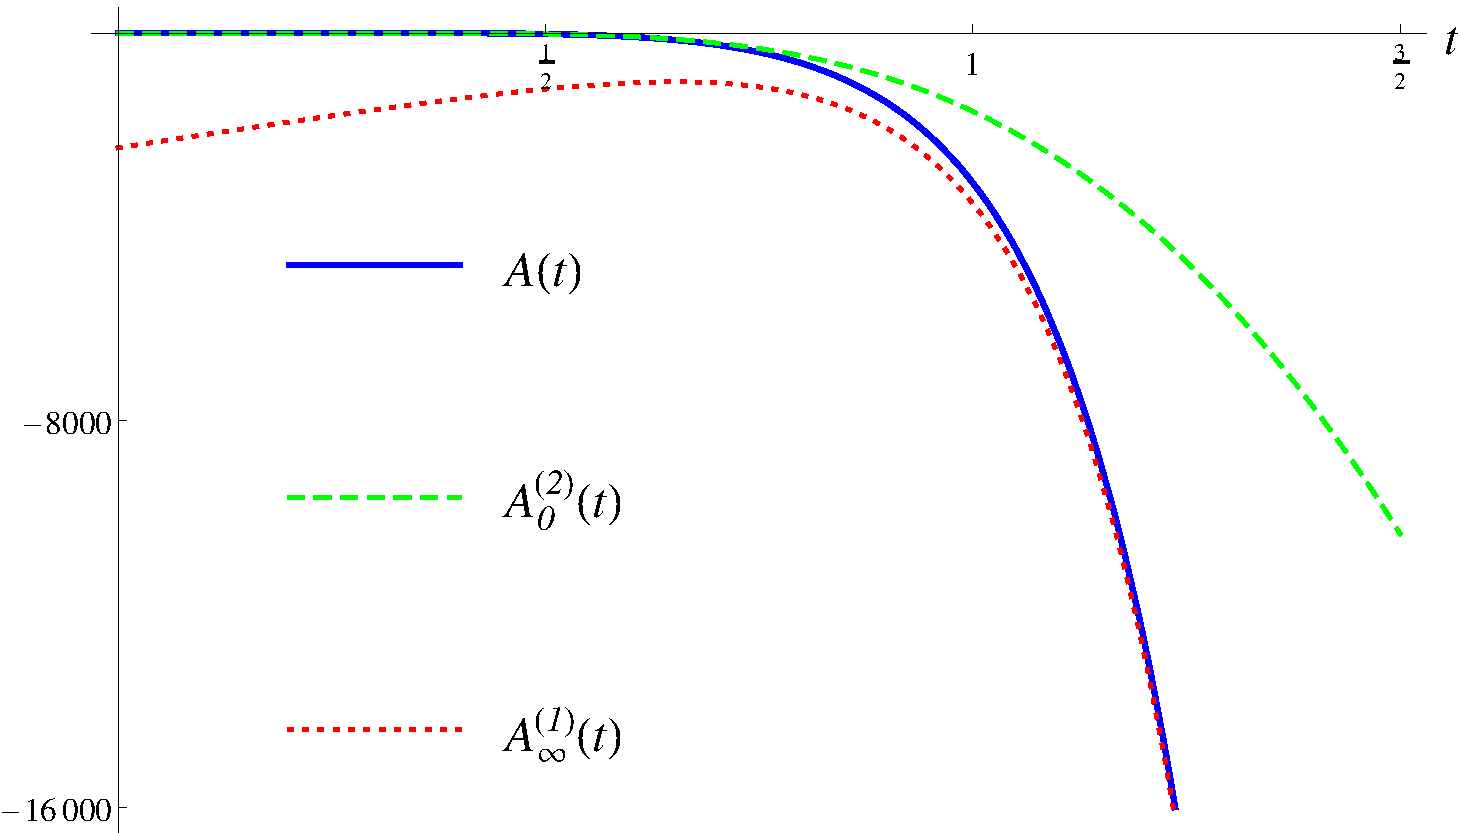
\includegraphics[width=300 pt]{graphics/e8plot_A.pdf}
\end{figure}

\noindent We observe that we can compute the values of $A(t)$ for $t\in(0,\infty)$ with any given precision. Indeed, from identities \eqref{eqn: phi0 transform} and \eqref{eqn: psi S define} we obtain the following two presentations for $A(t)$
\begin{align}
  A(t)=&-t^2\phi_0(i/t)+\frac{36}{\pi^2}\,t^2\,\psi_S(i/t)\notag\\
  A(t)=&-t^2\phi_0(it)+\frac{12}{\pi}\,t\,\phi_{-2}(it)-\frac{36}{\pi^2}\,\phi_{-4}(it)-\frac{36}{\pi^2}\,\psi_I(i/t).\notag
\end{align}
For an integer $n\geq0$ let $A_0^{(n)}$ and  $A_{\infty}^{(n)}$ be the functions such that
\begin{align}
  A(t)=&A_0^{(n)}(t)+O(t^2\,e^{-\pi n /t})\quad\mbox{as}\;t\to0\label{eqn: A asymptotic expansion 0}\\
  A(t)=&A_\infty^{(n)}(t)+O(t^2\,e^{-\pi n t})\quad\mbox{as}\;t\to\infty.\label{eqn: A asymptotic expansion infty}
\end{align}
For each $n\geq 0$ we can compute these functions from the Fourier expansions \eqref{eqn: phi fourier0}--\eqref{eqn: phi fourier4}, \eqref{eqn: psi fourier I}, and \eqref{eqn: psi fourier S}.
  For example, from \eqref{eqn: phi fourier4}--\eqref{eqn: phi fourier0} and \eqref{eqn: psi fourier I} we compute
%$$A_\infty^{(0)}(t)=-\frac{72}{\pi^2}\,e^{2\pi t}$$ and
\begin{align}A_\infty^{(6)}(t)=&\scriptstyle-\tfrac{72}{\pi ^2}\, e^{2 \pi  t}-\tfrac{23328}{\pi ^2}+\tfrac{184320}{\pi ^2}\, e^{-\pi  t}-\tfrac{5194368}{\pi ^2}\, e^{-2 \pi  t}+\tfrac{22560768}{\pi ^2}\, e^{-3 \pi  t}-\tfrac{250583040}{\pi
    ^2}\, e^{-4 \pi  t}+\tfrac{869916672 }{\pi ^2}\,e^{-5 \pi  t}\notag\\&\scriptstyle+t(\tfrac{8640}{\pi }+\tfrac{2436480}{\pi }\, e^{-2 \pi  t}+\tfrac{113011200 }{\pi }\,e^{-4 \pi  t})-t^2(518400\,e^{-2 \pi  t}+31104000\,e^{-4 \pi  t}).\notag
\end{align}
From \eqref{eqn: phi fourier4}--\eqref{eqn: phi fourier0} and \eqref{eqn: psi fourier S} we compute
%$$A_0^{(2)}(t)=-\frac{368640}{\pi^2}\,t^2\,e^{-\pi /t}$$and
$$A_0^{(6)}(t)=t^2(-\tfrac{368640}{\pi ^2}\, e^{-\pi/t}-518400\, e^{-2\pi/t}-\tfrac{45121536}{\pi ^2}\, e^{-3\pi/t}-31104000\,e^{-4\pi/t}-\tfrac{1739833344}{\pi ^2}\, e^{-5\pi/t}).$$
Moreover, from the convergent asymptotic expansion for the Fourier coefficients of a weakly holomorphic modular form \cite[Proposition 1.12]{Bruinier} we find that the $n$-th Fourier coefficient $c_{\psi_I}(n)$ of $\psi_I$ satisfies
\begin{equation}\label{eqn: Fourier estimate 1}|c_{\psi_I}(n)|\leq e^{4\pi\sqrt{n}}\qquad n\in\tfrac 12 \Z_{>0}.\end{equation} Similar inequalities hold for the Fourier coefficients of $\psi_S$, $\phi_0$, $\phi_{-2}$, and $\phi_{-4}$:
\begin{align}\label{eqn: Fourier estimate 2}
&|c_{\psi_S}(n)|\leq 2e^{4\pi\sqrt{n}}\qquad n\in\tfrac 12 \Z_{>0} \\
&|c_{\phi_0}(n)|\leq 2e^{4\pi\sqrt{n}}\qquad n\in \Z_{>0} \\
&|c_{\phi_{-2}}(n)|\leq e^{4\pi\sqrt{n}}\qquad n\in  \Z_{>0} \\
&|c_{\phi_{-4}}(n)|\leq e^{4\pi\sqrt{n}}\qquad n\in \Z_{>0}. \label{eqn: Fourier estimate 5}
  \end{align}
Therefore, we can estimate the error terms in the asymptotic expansions \eqref{eqn: A asymptotic expansion 0} and \eqref{eqn: A asymptotic expansion infty} of $A(t)$
\begin{align}
\left|A(t)-A_0^{(m)}(t)\right|\leq& (t^2+\frac{36}{\pi^2})\,\sum_{n=m}^\infty 2e^{2\sqrt{2}\pi\sqrt{n}}\,e^{-\pi n/t}\notag\\
\left|A(t)-A_\infty^{(m)}(t)\right|\leq& (t^2+\frac{12}{\pi}\,t+\frac{36}{\pi^2})\,\sum_{n=m}^\infty 2e^{2\sqrt{2}\pi\sqrt{n}}\,e^{-\pi nt}.\notag
\end{align}
  For an integer $m\geq0$ we set
\begin{align}
R^{(m)}_0:=&(t^2+\frac{36}{\pi^2})\,\sum_{n=m}^\infty 2e^{2\sqrt{2}\pi\sqrt{n}}\,e^{-\pi n/t}\notag\\
R^{(m)}_\infty:=&(t^2+\frac{12}{\pi}\,t+\frac{36}{\pi^2})\,\sum_{n=m}^\infty 2e^{2\sqrt{2}\pi\sqrt{n}}\,e^{-\pi nt}.\notag
\end{align}
Using interval arithmetic we check that
\begin{align}
&\left|R_0^{(6)}(t)\right|\leq\left|A_0^{(6)}(t)\right|\quad\mbox{ for }\;t\in(0,1]\notag\\
&\left|R_\infty^{(6)}(t)\right|\leq\left|A_\infty^{(6)}(t)\right|\quad\mbox{ for }\;t\in[1,\infty)\notag\\
&A_0^{(6)}(t)<0\quad\mbox{ for }\;t\in(0,1]\notag\\
&A_\infty^{(6)}(t)<0\quad\mbox{ for }\;t\in[1,\infty).\notag
\end{align}
Thus, we see that $A(t)<0$ for $t\in (0,\infty)$. Then identity \eqref{eqn: g A} implies \eqref{eqn: g1}.


Next, we prove \eqref{eqn: g2}. By Propositions~\ref{prop: a another integral} and~\ref{prop: b another integral} we know that for $r>0$
\begin{equation}\label{eqn: g B} \widehat{g}(r)=\frac{\pi}{2160}\,\sin(\pi r^2/2)^2\,\int\limits_0^\infty B(t)\,e^{-\pi r^2 t}\,dt\end{equation}
where $$B(t)=-t^2\phi_0(i/t)+\frac{36}{\pi^2}\,\psi_I(it).$$
This function can be also written as
\begin{align}
  B(t)=&-t^2\phi_0(i/t)-\frac{36}{\pi^2}\,t^2\,\psi_S(i/t)\notag\\
  B(t)=&-t^2\phi_0(it)+\frac{12}{\pi}\,t\,\phi_{-2}(it)-\frac{36}{\pi^2}\,\phi_{-4}(it)+\frac{36}{\pi^2}\,\psi_I(i/t).\notag
\end{align}
Our aim is to prove that $B(t)>0$ for $t\in(0,\infty)$. A plot of $B(t)$ is given in Figure~\ref{fig:B}.
\begin{figure}[h!]
\caption{Plot of the functions $B(t)$, $B^{(2)}_0(t)=\frac{368640}{\pi^2}\,t^2\,e^{-\pi /t}$, and $B^{(1)}_\infty(t)=\frac{8640}{\pi}t-\frac{23328}{\pi^2}$.\label{fig:B}}
  \centering
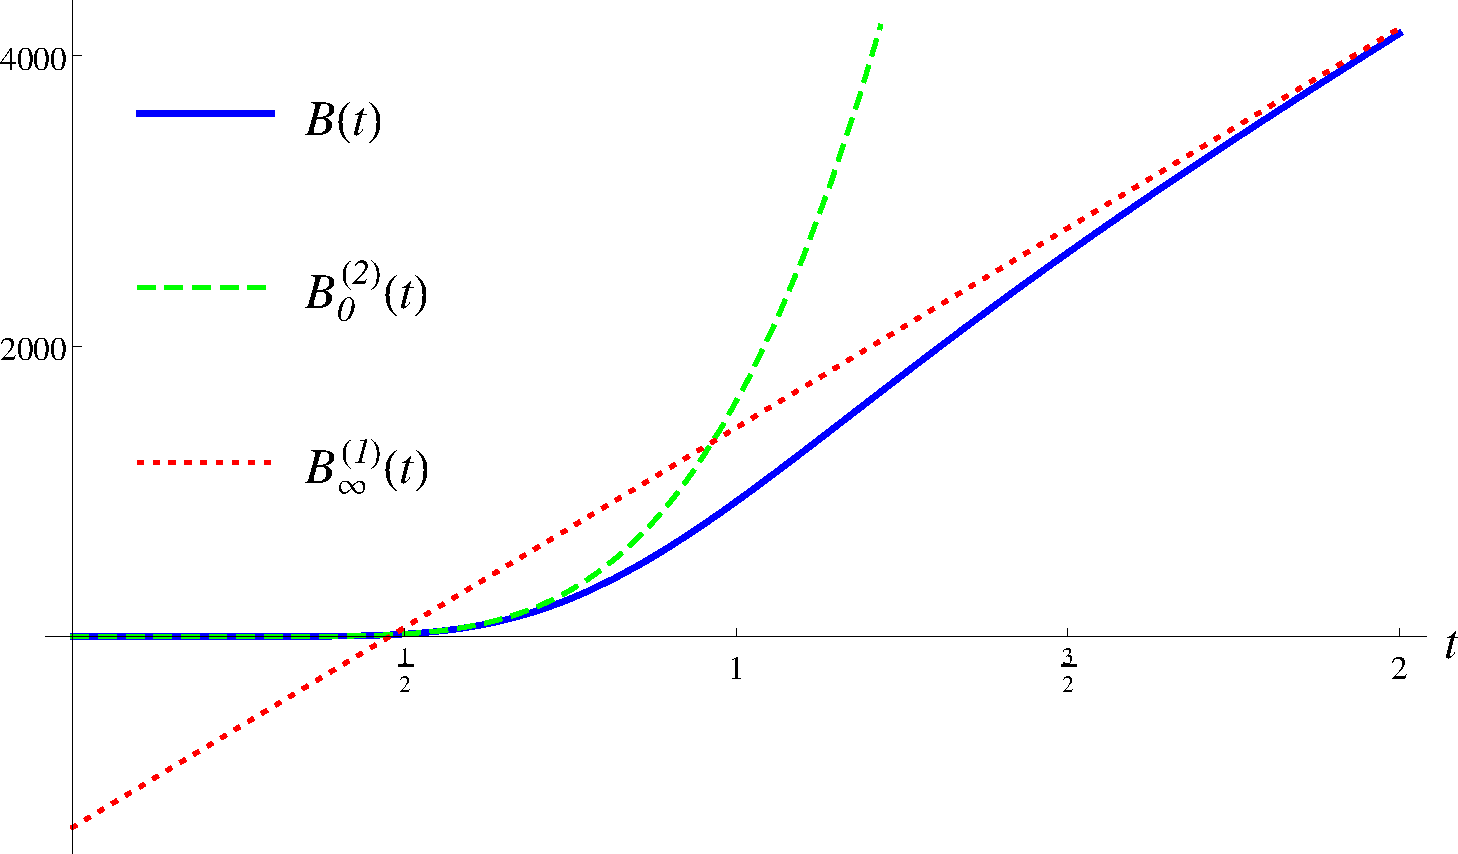
\includegraphics[width=300 pt]{graphics/e8plot_B.pdf}
\end{figure}

\noindent For $n\geq 0$ let $B_0^{(n)}$ and  $B_{\infty}^{(n)}$ be the functions  such that
\begin{align}
  B(t)=&B_0^{(n)}(t)+O(t^2\,e^{-\pi n /t})\quad\mbox{as}\;t\to0\notag\\
  B(t)=&B_\infty^{(n)}(t)+O(t^2\,e^{-\pi n t})\quad\mbox{as}\;t\to\infty.\notag
\end{align}
We find
\begin{align}B_\infty^{(6)}(t)=&-\tfrac{12960}{\pi ^2}-\tfrac{184320}{\pi ^2}\,\scriptstyle e^{-\pi  t}\displaystyle-\tfrac{116640}{\pi ^2} \,\scriptstyle e^{-2\pi  t}\displaystyle-\tfrac{22560768}{\pi ^2}\,\scriptstyle e^{-3\pi  t}\displaystyle+\tfrac{56540160}{\pi ^2}\,\scriptstyle e^{-4\pi  t}\displaystyle-\tfrac{869916672 }{\pi ^2} \,\scriptstyle e^{-5\pi  t}\displaystyle\notag\\
&+t(\tfrac{8640 }{\pi }+\tfrac{2436480}{\pi }\,\scriptstyle e^{-2\pi  t}\displaystyle+\tfrac{113011200 }{\pi }\,\scriptstyle e^{-4\pi  t}\textstyle)-t^2(\scriptstyle518400\,\scriptstyle e^{-2\pi  t}\displaystyle+\scriptstyle31104000\,\scriptstyle e^{-4\pi  t}\displaystyle)\notag
\end{align}
and
$$B_0^{(6)}(t)= t^2(\tfrac{368640}{\pi ^2}\, e^{-\pi/t}-518400\, e^{-2 \pi /t}+\tfrac{45121536 }{\pi ^2}\,e^{-3 \pi/t}-31104000\, e^{-4 \pi/t}+\tfrac{1739833344 }{\pi ^2}\,e^{-5 \pi/t}) .$$
The estimates \eqref{eqn: Fourier estimate 1}--\eqref{eqn: Fourier estimate 5} imply that $$\left|B(t)-B_0^{(6)}(t)\right|\leq R_0^{(6)}(t)\quad\mbox{for}\;t\in(0,1]$$
and
$$\left|B(t)-B_\infty^{(6)}(t)\right|\leq R_\infty^{(6)}(t)\quad\mbox{for}\;t\in[1,\infty).$$
Using interval arithmetic we verify that
\begin{align}
&\left|R_0^{(6)}(t)\right|\leq\left|B_0^{(6)}(t)\right|\quad\mbox{ for }\;t\in(0,1]\notag \\
&\left|R_\infty^{(6)}(t)\right|\leq\left|B_\infty^{(6)}(t)\right|\quad\mbox{ for }\;t\in[1,\infty)\notag \\
&B_0^{(6)}(t)>0\quad\mbox{ for }\;t\in(0,1]\notag \\
&B_\infty^{(6)}(t)>0\quad\mbox{ for }\;t\in[1,\infty). \notag
\end{align}
Now identity \eqref{eqn: g B} implies \eqref{eqn: g2}.

Finally, the property \eqref{eqn: g3} readily follows from Proposition~\ref{prop: a values} and Proposition~\ref{prop: b values}.
This finishes the proof of Theorems~\ref{thm: g1} and~\ref{thm: g}.
  \end{proof}




\begin{thebibliography}{10}
\bibitem{Abramowitz} {\sc M. Abramowitz, I. Stegun}, \emph{ Handbook of Mathematical Functions with Formulas, Graphs, and Mathematical Tables}, Applied Mathematics Series 55 (10 ed.), New York, USA: United States Department of Commerce, National Bureau of Standards; Dover Publications, 1964.

%\bibitem{BRV} {\sc A. Bondarenko, D. Radchenko, M. Viazovska}, \emph{On optimal asymptotic bounds for spherical designs}, Annals of Math. 178 (2)(2013), pp. 443--452.

\bibitem{Bruinier} {\sc J. Bruinier}, \emph{Borcherds products on O(2,l) and Chern classes of Heegner divisors}, Springer Lecture Notes in Mathematics 1780 (2002)

\bibitem{ElkiesCohn}  {\sc H. Cohn, N. Elkies}, \emph{New upper bounds on sphere packings I}, Annals of Math. 157 (2003) pp. 689--714.

%\bibitem{Cohn} {\sc H. Cohn}, \emph{New upper bounds on sphere packings. II.} Geom. Topol. 6 (2002), pp. 329--353.

%\bibitem{CohnKumar} {\sc H. Cohn, A. Kumar}, \emph{Universally optimal distribution of points on spheres}, J. Amer. Math. Soc. 20 (1) (2007), pp. 99--148.

%\bibitem{ConwaySloan}  {\sc J. H. Conway and N. J. A. Sloane}, \emph{What Are All the Best Sphere Packings in Low Dimensions? ,} Discrete Comput. Geom. (Laszlo Fejes Toth Festschrift), 13 (1995), pp. 383--403.


%\bibitem{DukeImamogluToth} {\sc W. Duke, O. Imamoglu and A. Toth}, {\em Cycle integrals of the j-function and mock modular forms}, Ann. of Math. (2) 173 (2011), no. 2, 947-981.

%\bibitem{Deligne1} {\sc P. Deligne}, \emph{Travaux de Shimura.} S\'eminaire Bourbaki, 23\'eme ann\'ee (1970/71), Exp. No. 389, pp. 123-165. Lecture Notes in Math., Vol. 244, Springer, Berlin, 1971.

%\bibitem{Deligne2} {\sc P. Deligne}, \emph{Vari\'et\'es de Shimura: interpr\'etation modulaire, et techniques de construction de mod\'eles canoniques}, in Automorphic forms, representations and L-functions, Proc. Sympos. Pure Math., XXXIII (Corvallis, OR, 1977), Part 2, pp. 247-289, Amer. Math. Soc., Providence, R.I., 1979.



%\bibitem{CohnZ} {\sc H. Cohn, Y. Zhao}, \emph{Sphere packing bounds via spherical codes}, arXiv:1212.5966 [math.MG]

%\bibitem{Delsarte72} {\sc P. Delsarte},\emph{Bounds for unrestricted codes, by linear programming}, Philips Res. Rep. 27 (1972), pp. 272--289.


%\bibitem{Delsarte77} {\sc P. Delsarte, J. M. Goethals, and J. J. Seidel}, \emph{Spherical codes and designs}, Geom. Dedicata, 6 (1977), pp. 363--388.

\bibitem{first course} {\sc F. Diamond, J. Shurman}, \emph{A First Course in Modular Forms}, Springer New York, 2005.

%\bibitem{Toth} {\sc L. Fejes Toth}, {\em {\"U}ber die dichteste Kugellagerung}, Math. Z. 48 (1943), pp. 676--684.

%\bibitem{Hales} {\sc T. Hales}, {\em A proof of the Kepler conjecture}, Annals of Math. 162 (3) (2005), pp. 1065--1185.

\bibitem{Hejhal} {\sc D. Hejhal}, {\em The Selberg trace formula for $\mathrm{PSL}(2, \R)$},  Springer Lecture Notes in Mathematics 1001 (1983)

%\bibitem{KabLev} {\sc G. A. Kabatiansky and V. I. Levenshtein}, {\em Bounds for packings on a sphere and in space},Problems of Information Transmission 14 (1978), pp. 1--17.

\bibitem{Mumford} {\sc D. Mumford}, {\em Tata Lectures on Theta I}, Birkh\"auser, 1983.

%\bibitem{Ma} {\sc Manin, Yu. I.}, {\em Real multiplication and noncommutative geometry (ein Alterstraum)}. The legacy of Niels Henrik Abel, 685-727, Springer, Berlin, 2004.

%\bibitem{MaOdSl} {\sc C. L. Mallows, A. M. Odlyzko, and N. J. A. Sloane}, {\em Upper bounds for modular forms, lattices, and codes}, J. Algebra, 36 (1975), 68--76

\bibitem{Petersson32} {\sc H. Petersson}, {\em Ueber die Entwicklungskoeffizienten der automorphen Formen}, Acta Mathematica, Bd. 58 (1932),  pp. 169--215.

%\bibitem{PfenderZiegler} {\sc F. Pfender, G. M. Ziegler,} {\em Kissing numbers, sphere packings, and some unexpected proofs}, Notice of the AMS  51 (8) (2004) pp. 873--883

\bibitem{Rademacher38} {\sc H. Rademacher and H. S. Zuckerman}, {\em On the Fourier coefficients of certain modular forms of
positive dimension}, Annals of Math. (2) 39 (1938),  pp. 433--462.

%\bibitem{Thue} {\sc A. Thue}, {\em {\"U}ber die dichteste Zusammenstellung von kongruenten Kreisen in einer Ebene}, Norske Vid. Selsk. Skr. No.1 (1910), pp. 1--9.

%\bibitem{Venk}   {\sc  A. Venkatesh}, {\em A Note on Sphere Packings in High Dimension}, International Mathematics Research Notices  7 (2013),  1628--1642

%\bibitem{Yudin} {\sc V. A. Yudin}, {\em Lower bounds for spherical designs}, Izv. Ross. Akad. Nauk. Ser. Mat. 61 (1997), pp. 211-233. English transl., Izv. Math. 6 (1997), pp. 673--683.

\bibitem{1-2-3} {\sc D. Zagier}, {\em Elliptic Modular Forms and Their Applications}, In:  The 1-2-3 of Modular Forms, (K. Ranestad, ed.) Norway, Springer Universitext, 2008.
\end{thebibliography}

\newpage

{\footnotesize
\noindent
Ecole Polytechnique Federale de Lausanne\\
1015 Lausanne\\
Switzerland\\
{\it Email address: maryna.viazovska@epfl.ch}}

\end{document}
